\documentclass[11pt,twocolumn]{article}

\usepackage{titlesec}
\usepackage[hyphens]{url}

\newsavebox{\tempbox}
\sbox{\tempbox}{\raisebox{-4.5pt}%
{\parbox{3cm}{\textit{\textbf{{\large ``Channel \hspace{1em} Abstractions"}}}}}}

%\newsavebox{\sstwolinebox}
%\sbox{\sstwolinebox}{\raisebox{-5pt}%
%{\parbox{7.4cm}{\textit{\textbf{{\large %
%Range-Bounded Types, Value Constructors, and Addressability}}}}}}
%\newcommand{\sstwoline}{\usebox{\sstwolinebox}}

%\definecolor{midRed}{rgb}{.5,.0,.25}
%\definecolor{logoRed}{rgb}{.3,0,0}



\newenvironment{displayquotexxx}{%
	%\begin{fcolorbox}{yellow!20!gray}{red!5}
	\begin{flushright}
	\begin{tcolorbox}[
		colback=gray!4,
		colframe=red!20!gray,
		width=.98\linewidth,
		boxrule=1pt,leftrule=3pt,
		rightrule=1pt,toprule=.5pt,arc=0pt,auto outer arc
		]
\begin{minipage}{21.5em}}{%
\end{minipage}\end{tcolorbox}
	\end{flushright}
}

\usepackage{changepage}

\newenvironment{dquote}{%
	%\begin{fcolorbox}{yellow!20!gray}{red!5}
	\begin{flushright}
	\vspace{1em}\begin{tcolorbox}[
		breakable, parbox=false, colback=gray!4,
		colframe=mRed!20!gray,
		width=.995\linewidth,
		boxrule=1pt,leftrule=3pt,
		rightrule=1pt,toprule=.5pt,arc=0pt,auto outer arc
		]
\begin{adjustwidth}{1pt}{-3pt}
}{%
\end{adjustwidth}
\end{tcolorbox}\vspace{1em}
	\end{flushright}
}



\newcounter{subs}[section]

\newcommand{\subss}[2]{	
\phantomsection \label{#1}
\addcontentsline{toc}{subsection}{#1}
\stepcounter{subs}
\refstepcounter{subsection}
\vspace*{3.25em}

\noindent{ {\Large\textbf\thesection.}{\large\textbf\thesubs}} {
 {{\Large\textbf #2}}
}
\vspace*{.35em} 
}

\newcommand{\subsstlx}[2]{}

\newcommand{\subsstl}[2]{	
\phantomsection \label{#1}
\addcontentsline{toc}{subsection}{#1}
\stepcounter{subs}
\refstepcounter{subsection}
\vspace*{3.25em}

\noindent{ \raisebox{-1pt}{\Large\textbf\thesection.}{\large\textbf\thesubs}} {
\raisebox{-1pt}{{\Large\textbf #2}}
}
\vspace*{.35em} 
}

\newcommand{\subsstly}[2]{	
\phantomsection \label{#1}
\addcontentsline{toc}{subsection}{#1}
\stepcounter{subs}
\refstepcounter{subsection}
\vspace*{3.25em}

\noindent{ \raisebox{-1pt}{\Large\textbf\thesection.}{\large\textbf\thesubs}} {
\raisebox{-1pt}{{\Large\textbf #2}}
}
\vspace*{.35em} 
}


\let\Osubsection\subsection

\renewcommand{\subsection}[1]{\subss{#1}{#1}}

\newcommand{\subsectionalt}[2]{\subss{#1}{#2}}


\newsavebox{\twolinebox}

\newcommand{\stwoline}[1]{%
\sbox{\twolinebox}{\raisebox{-3pt}%
{\parbox{7.4cm}{\linespread{1.25}\selectfont\raggedleft{\textbf{{\large #1}}}}}}}

\newcommand{\twoline}{\usebox{\twolinebox}}

\newcommand{\subsectiontwoline}[1]{\stwoline{#1}\subsstl{#1}{\twoline}

\vspace{1em}}

\newcommand{\spsubsectiontwolinerepl}[2]{\stwoline{#1}\subsstl{#2}{\twoline}}
\newcommand{\subsectiontwolinerepl}[2]{\stwoline{#1}\subsstl{#2}{\twoline}

\vspace{1em}}

\newcommand{\subsectiontwolinealt}[2]{\stwoline{#1}\subsstl{#2}{\twoline}

\vspace{1em}}


\titlespacing{\subsection}{0pt}{20pt}{20pt}
\titlespacing{\section}{0pt}{35pt}{15pt}
\titlespacing{\subsubsection}{0pt}{20pt}{5pt}


\newcommand{\spsubsection}[1]{%
\subss{#1}{#1}
\vspace{1em}
}
\newcommand{\spsubsectiontwoline}[1]{%
\subsectiontwoline{#1}
\vspace{1em}
}



\usepackage{csquotes}

\usepackage{booktabs}

\usepackage{amssymb}

\usepackage{titlesec}

\usepackage{transparent}

\usepackage{setspace}

\usepackage{graphicx}

\newcommand{\sectionGraphics}{

\vspace{2em}\centerline{\includegraphics[scale=0.125]{logo-deco.png}}\vspace{-1em}}

\usepackage[flushmargin]{footmisc}

\setlength{\parindent}{30pt}

\usepackage[letterpaper, left=.47in,right=.47in,top=.825in,bottom=.825in]{geometry}

\let\xbibitem\bibitem
\renewcommand{\bibitem}[2]{\vspace{6.5pt}\xbibitem{#1}{#2}}

\newenvironment{frquote}{%
%\begin{fcolorbox}{yellow!20!gray}{red!5}
%\begin{flushright}

\begin{tcolorbox}[
	colback=white,
	colframe=white,
	width=.97\linewidth,
	arc=0mm, auto outer arc
	]
\begin{scriptsize}
\begin{minipage}{61em}
\begin{flushright}
\begin{minipage}{63em}}{%
\end{minipage}
\end{flushright}
\end{minipage}
\end{scriptsize}
\end{tcolorbox}
%\end{flushright}
}

%\colorlet{codegr}{black!80!blue}

\setlength{\columnsep}{8mm}

\usepackage{etoolbox}

\AtBeginEnvironment{thebibliography}{\linespread{1}\selectfont}

\usepackage{mathptmx}

\titleformat*{\subsection}{\small\bfseries}

\usepackage{wasysym}
\usepackage{textcomp}
\usepackage{amssymb}

\usepackage{microtype}

\DeclareMathAlphabet{\mathcal}{OMS}{cmsy}{m}{n}

\let\OldI\i

\newcommand{\secvspace}{\vspace{-0.3em}}
\newcommand{\asecvspace}{\vspace{-0.05em}}

\newcommand{\mdash}{---}
\newcommand{\q}[1]{``#1"}
\newcommand{\sq}[1]{`#1'}
\renewcommand{\i}[1]{\textit{#1}}

\newcommand{\nl}{

}

\newcommand{\T}[1]{\raisebox{-2pt}{\ensuremath{\mathcal{T}}}\textit{\tiny #1}}

\newcommand{\biburl}[1]{ {\fontfamily{gar}\selectfont{\textcolor[rgb]{.2,.6,0}%
{\scriptsize {\url{#1}}}}}}

%\newcommand{\biburl}[1]{ {\fontfamily{gar}\selectfont{\textcolor[rgb]%%{.2,.6,0}%
%{\scriptsize \textls*[-70]{\burl{#1}}}}}}

\newcommand{\TSupT}{\ensuremath{{\T2}\makebox[4pt][r]{\raisebox{5pt}{{\scalebox{.6}{\T1}}}}}}

\let\OldFootnoteSize\footnotesize
\renewcommand{\footnotesize}{\scriptsize}

\newcommand{\emigres}{\'emigr\'es}

\newcommand{\SExpressions}{S-Expressions}
\newcommand{\SExpression}{S-Expression}

\newcommand{\cq}[1]{{\fontfamily{gar}\selectfont ``}#1{\fontfamily{gar}\selectfont "}}

\newcommand{\Retore}{Retor\'e}
\newcommand{\Aurelie}{Aur\'elie}
\newcommand{\Descles}{D\'escles}

\newcommand{\SG}{\ensuremath{\mathbb{SG}}}
\newcommand{\tLa}{\ensuremath{\mathbb{A}_\lambda}}

\newcommand{\lt}{\ensuremath{<}}
\newcommand{\ancestorLt}{\ensuremath{\lll}}
\newcommand{\aALTb}{\ensuremath{a {\lll} b}}
\newcommand{\aLTb}{\ensuremath{a {\lt} b}}
\newcommand{\aLTcLtb}{\ensuremath{a {\lt} b {\lt} c}}
\newcommand{\aDLTb}{\ensuremath{a {\lessdot} b}}

\newcommand{\aMath}{\ensuremath{a}}
\newcommand{\bMath}{\ensuremath{b}}
\newcommand{\cMath}{\ensuremath{c}}

\newcommand{\ala}{\`a la}

\newcommand{\br}{

}


\newcommand{\CppEleven}{{\Cpp}11}

\usepackage{graphicx}

\usepackage[breakable]{tcolorbox}

\newsavebox\lstbox



\newif\iffootnote
\let\Footnote\footnote
\renewcommand\footnote[1]{\begingroup\footnotetrue\Footnote{#1}\endgroup}

\colorlet{orr}{orange!60!red}

\newcommand{\textscc}[1]{{\color{orr!35!black}{{%
						\fontfamily{Cabin-TLF}\fontseries{b}\selectfont{\textsc{#1}}}}}}

\newcommand{\textscnc}[1]{{%
						\fontfamily{Cabin-TLF}\fontseries{b}\selectfont{\textsc{#1}}}}

\newcommand{\AcronymTextNC}[1]{{\iffootnote\begin{footnotesize}{\textscnc{#1}}\end{footnotesize}%
\else\begin{small}{\textscnc{#1}}\end{small}\fi}}

\newcommand{\AcronymText}[1]{{\iffootnote\begin{scriptsize}{\textscc{#1}}\end{scriptsize}%
\else\begin{OldFootnoteSize}{\textscc{#1}}\end{OldFootnoteSize}\fi}}

\newcommand{\smAcronymText}[1]{\begin{footnotesize}\textscc{#1}\end{footnotesize}}

\newcommand{\librets}{\AcronymText{librets}}
\newcommand{\FHIR}{\AcronymText{FHIR}}
\newcommand{\DICOM}{\AcronymText{DICOM}}

\newcommand{\IoT}{\AcronymText{IoT}}


\newcommand{\TCP}{\AcronymText{TCP}}
\newcommand{\GPS}{\AcronymText{GPS}}
\newcommand{\CppTwenty}{\AcronymText{C++20}}

\newcommand{\AcronymTextInitialCap}[1]{{\iffootnote\begin{scriptsize}{\textsc{#1}}\end{scriptsize}%
		\else\begin{normalsize}{\textsc{#1}}\end{normalsize}\fi}}


\newcommand{\rel}[1]{\raisebox{0.25pt}{%
	{\iffootnote\begin{footnotesize}{\textsc{#1}}\end{footnotesize}%
		\else\begin{OldFootnoteSize}{\textsc{#1}}\end{OldFootnoteSize}\fi}}}

\newcommand{\vs}{

\vspace*{0.2em}}


\newcommand{\HTML}{\AcronymText{HTML}}

\newcommand{\UX}{\AcronymText{UX}}

\newcommand{\Csh}{\AcronymText{C\#}}

\newcommand{\PHP}{\AcronymText{PHP}}
\newcommand{\IDE}{\AcronymText{IDE}}

\newcommand{\AND}{\AcronymText{AND}}
\newcommand{\DX}{\AcronymText{DX}}

\newcommand{\RelaeGraph}{\AcronymText{RelaeGraph}}
\newcommand{\PDF}{\AcronymText{PDF}}

\newcommand{\NDP}{\AcronymText{NDP}}
\newcommand{\UML}{\AcronymText{UML}}
\newcommand{\GIT}{\AcronymText{GIT}}

\newcommand{\UI}{\AcronymText{UI}}
\newcommand{\QML}{\AcronymText{QML}}

\newcommand{\SPARQL}{\AcronymText{SPARQL}}
\newcommand{\OWL}{\AcronymText{OWL}}
\newcommand{\JSON}{\AcronymText{JSON}}

\newcommand{\const}{\AcronymText{const}}
\newcommand{\GeCODE}{\AcronymText{GeCODE}}

\newcommand{\Python}{\AcronymText{Python}}


\newcommand{\GUI}{\AcronymText{GUI}}
\newcommand{\BNF}{\AcronymText{BNF}}


\newcommand{\NLP}{\AcronymText{NLP}}

\newcommand{\Francois}{Fran\c{}cois}


\newcommand{\Gardenfors}{G\"ardenfors}


\newcommand{\Haskell}{\AcronymText{Haskell}}

\newcommand{\Cpp}{\AcronymText{C++}}
\newcommand{\RDF}{\AcronymText{RDF}}
\newcommand{\Java}{\AcronymText{Java}}
\newcommand{\IT}{\AcronymText{IT}}
\newcommand{\AI}{\AcronymText{AI}}

\newcommand{\SCA}{\AcronymText{SCA}}

\newcommand{\Lisp}{\AcronymText{Lisp}}

\newcommand{\Scheme}{\AcronymText{Scheme}}

\newcommand{\ThreeD}{\AcronymText{3D}}

\definecolor{DarkRed}{rgb}{.2,.0,.1}

\colorlet{orrr}{orange!40!red}
\colorlet{orrbl}{orrr!85!blue}
\colorlet{orrb}{orrbl!80!DarkRed}

\newcommand{\lclc}[1]{{\color{orrb}{#1}}}

\newcommand{\lcl}[2]{{\resizebox{!}{#1}{\color{orrb}{#2}}}}
\newcommand{\ty}{{\lcl{8pt}{\ensuremath{\mathfrak{t}}}}}

\newcommand{\caltypeT}{\ensuremath{\ty}}
\newcommand{\calS}{\ensuremath{\mathcal{S}}}

\newcommand{\typeTp}{\lclc{\ensuremath{\ty'}}}
\newcommand{\typeTpp}{\lclc{\ensuremath{\ty''}}}


\newcommand{\gOpTransferOneOneF}{\codeText{g:}\codeTextr{return$_1$}{\opTransfer}%
\codeText{f:}\codeTextr{lambda$_1$}}
 
\newcommand{\fDotOfg}{\codeText{f$\circ$g}}
\newcommand{\fDotOfGX}{\codeText{(f.g)(x)}}
\newcommand{\fOfGx}{\codeText{f(g(x))}}

\newcommand{\fgx}{\codeText{f(g(x))}}

\newcommand{\funG}{\codeText{g}}
\newcommand{\funF}{\codeText{f}} 

\newcommand{\tyOne}{\codeText{${\ty}_1$}}
\newcommand{\tyTwo}{\codeText{${\ty}_2$}}

\newcommand{\tyOneTotyTwo}{\tyOne \codeText{$\rightarrow$} \tyTwo}

\newcommand{\chK}{\codeText{$\mathcal{K}$}}

\newcommand{\tOneTimesTTwo}{\codeText{${\ty}_1$ $\times$ ${\ty}_2$}}
\newcommand{\tOneTimesTOne}{\codeText{${\ty}_1$ $\times$ ${\ty}_1$}}
\newcommand{\tyOneTimesTyTwo}{\codeText{${\ty}_1$ $\times$ ${\ty}_2$}}

\newcommand{\tOneTimesTTwoToTOneOntoTTwo}{\codeText{${\ty}_1$ $\times$ ${\ty}_2$ %
$\Longrightarrow$ ${\ty}_1$ $\rightarrow$ ${\ty}_2$}}

\newcommand{\unitTy}{\codeText{Unit}} 
\newcommand{\unitVal}{\codeText{unit}} 

\newcommand{\unitTyToty}{\unitTy{}{ }%
\codeText{$\rightarrow$ {\ty}}}

\newcommand{\tyOneToTyTwo}{\codeText{${\ty}_1$ $\rightarrow$ ${\ty}_2$}}

\newcommand{\tyE}{\lclc{$E$}}
\newcommand{\tyTotyE}{\codeText{{\ty} $\rightarrow$ $E$}}
\newcommand{\tyToTyE}{\codeText{{\ty} $\rightarrow$ $E$}}
 
\newcommand{\tyValues}{{\ty}-values}


	
\newcommand{\Tnoindex}{\raisebox{-2pt}{\ensuremath\ty}}

\newcommand{\typeAbove}{%
\raisebox{-1pt}{\rotatebox{90}{\begin{tiny}$\diagdown$\makebox[1pt][c]{$\diagup$}\end{tiny}}}}

\newcommand{\typeT}{\ensuremath{type\raisebox{.5pt}{\makebox[3pt][c]{-}}\ty}}
\newcommand{\TValues}{{\ensuremath\ty}-values} 

\newcommand{\tOnetoTwotoThree}{\codeText{${\ty}_1$\smsp%
$\rightarrow$\smsp${\ty}_2$\smsp$\rightarrow$\smsp${\ty}_3$}}
 
\newcommand{\tOnetoTwoTOThree}{\codeText{${\ty}_1$\smsp%
$\rightarrow$\smsp\smsp(${\ty}_2$\smsp$\rightarrow$\smsp${\ty}_3$)}} 


\definecolor{BaseColor}{HTML}{8533FF}

\colorlet{ftcfore}{BaseColor!60!cyan}
\colorlet{ftcback}{BaseColor!40!cyan}

\newcommand{\ftc}[3]{
\vspace*{6mm}
\begin{tcolorbox}
[float=t, colframe=ftcfore!20!white,boxrule=0.5pt,arc=22pt,enhanced,
title={{\color{black}{\protect{#1}}}},label={#2}
toprule=0pt,bottomrule=1pt,
drop fuzzy shadow northeast={darkRed!40!ftcback},
      boxsep=3pt]\hspace{3em}\parbox{0.8\textwidth}\protect{#3}
\end{tcolorbox}      
\vspace*{-4mm}
}

\newcommand{\tc}[2]{
\vspace*{6mm}
\begin{tcolorbox}
[#1 colframe=darkRed!70!BaseColor,boxrule=0.5pt,arc=22pt,enhanced,
toprule=0pt,bottomrule=1pt,
drop fuzzy shadow northeast={darkRed!70!purple},
      boxsep=3pt]\hspace{3em}\parbox{0.8\textwidth}\protect{#2}
\end{tcolorbox}      
\vspace*{-4mm}
}

\tcbuselibrary{skins}
\usetikzlibrary{calc}
\usetikzlibrary{shadows}
\pgfdeclarelayer{background}
\pgfdeclarelayer{foreground}
\pgfsetlayers{background,main,foreground}



\usetikzlibrary{fit}
\usepackage{caption}

\renewcommand{\figurename}{Diagram}

\newcommand{\emblink}[2]{\href{#1}{#2}}

\newcommand{\tmphs}{\hypersetup{linkbordercolor=orange!50!red,linkcolor=black}}
\newcommand{\tmphscol}{\hypersetup{linkbordercolor=gray!40,linkcolor=black}}

\usepackage[object=vectorian]{pgfornament} 

\newcommand{\decoline}{\vspace{-4em}}

\newcommand{\decolinex}{%

\vspace{-2em}
{\color{darkRed!60!cyan}\noindent\hfil{\EnglischeLinie}\hfil}
\vspace{-2.25em}}


\newcommand{\whdecoline}{%

\vspace{-2em}
{\color{white}\noindent\hfil{\whEnglischeLinie}\hfil}
\vspace{-2.25em}}

\newcommand{\sectionline}[1]{%
  \noindent
  \begin{center}
  {\color{#1}
    \resizebox{0.5\linewidth}{1ex}
    {{%
    {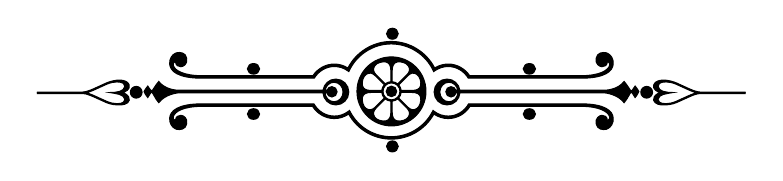
\begin{tikzpicture}
    \node  (C) at (0,0) {};
    \node (D) at (9,0) {};
    \path (C) to [ornament=84] (D);
    \end{tikzpicture}}}}}%
    \end{center}
  }
  
\newcommand{\EnglischeLinie}{
\sectionline{darkRed!60!cyan}
}

\newcommand{\whEnglischeLinie}{
\sectionline{white}
}

\newcommand{\thinsectionline}[1]{%
	\noindent
	\begin{center}
		{\color{#1}
			\resizebox{.2\linewidth}{1.5ex}
			{{%
					{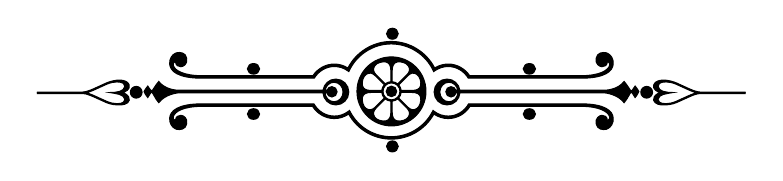
\begin{tikzpicture}
						\node  (C) at (0,0) {};
						\node (D) at (9,0) {};
						\path (C) to [ornament=84] (D);
						\end{tikzpicture}}}}}%
	\end{center}
}

\newcommand{\thindecolinex}{\vspace*{-.15em}\thinsectionline{blGreen!10!orange}\vspace*{-.45em}}
\newcommand{\thindecolineadjx}[2]{\vspace*{#1}\thinsectionline{blGreen!10!orange}\vspace*{#2}}


\newcommand{\thindecoline}{\vspace*{-.15em}\thinsectionline{black!70}\vspace*{-.45em}}
\newcommand{\thindecolineadj}[2]{\vspace*{#1}\thinsectionline{black!70}\vspace*{#2}}


\newlength{\mplength}
\setlength{\mplength}{1.05\linewidth}

\newlength{\hslength}
\setlength{\hslength}{-1.45cm}

\newcommand{\spinc}[1]{\input{#1}}

\newsavebox{\tcsb}


\newcommand{\spinctc}[3]{\begin{lrbox}{\tcsb}\protect\input{#1}\end{lrbox} %\input{#1}
\begin{figure}
\tc{}{\protect\usebox\tcsb} 
\captionof{figure}{#2}
\label{#3}
\end{figure}
}

\usetikzlibrary{backgrounds} 
\usetikzlibrary{arrows}
\tikzset{>=triangle 90}

\newcommand{\gFunB}{\ensuremath{\mathfrak{g}}}
\newcommand{\fFunB}{\ensuremath{\mathfrak{f}}}

%\newcommand{\lstinlinebstyle}[1]{\Colorbox{blue!10}{%
%		{\fontfamily{Cabin-TLF}\fontseries{b}\fontsize{9pt}{16pt}\selectfont{{\textls[200]{#1}}}}}}

\newcommand{\lstinlinebstyle}[1]{\textls[200]{#1}}


\newenvironment{tikzgrid}{%
\begin{tikzpicture}[shorten >=1pt,node distance=2cm,on grid,auto,
framed,background rectangle/.style={double,ultra thick,draw=darkRed, bottom color=cyan!20, 
	top color=black!20, rounded corners}]%
}{\end{tikzpicture}}
 
\usepackage[font=small,labelfont=bf]{caption}

\definecolor{BaseColor}{HTML}{8533FF}

\colorlet{ftcfore}{BaseColor!60!cyan}
\colorlet{ftcback}{BaseColor!40!cyan}


\newcommand{\tcl}[1]{\begin{lrbox}{\lstbox}\begin{minipage}{\mplength}
\input{#1}
\end{minipage}\end{lrbox}
\tc{}{\hspace*{\hslength}\usebox\lstbox}
}

\newcommand{\itcl}[1]{
\input{#1}
}

\newcommand{\itclfig}[2]{
\begin{figure}\input{#1}
\label{#2}
\end{figure}
}

\newcommand{\ftcl}[2]{\begin{lrbox}{\lstbox}\begin{minipage}{\mplength}
\input{#2}
\end{minipage}\end{lrbox}
\tc{float=#1,}{\hspace*{\hslength}\usebox\lstbox}
}

\newcommand{\vsftcl}[2]{\begin{lrbox}{\lstbox}\begin{minipage}{\mplength}
\vsinput{#2}
\end{minipage}\end{lrbox}
\tc{float=#1,}{\hspace*{\hslength}\usebox\lstbox}
}

\newcommand{\vstcl}[1]{\begin{lrbox}{\lstbox}\begin{minipage}{\mplength}
%\vsinput{#1}
\end{minipage}\end{lrbox}  
%\tc{}{\hspace*{\hslength}\usebox\lstbox}
}


\definecolor{blGreen}{rgb}{.2,.7,.3}
\definecolor{darkRed}{rgb}{.2,.0,.1}

\definecolor{darkBlGreen}{rgb}{.1,.3,.2}

\definecolor{oldBlColor}{rgb}{.2,.7,.3}

\definecolor{blColor}{rgb}{.1,.3,.2}

\definecolor{elColor}{rgb}{.2,.1,0}
\definecolor{flColor}{rgb}{0.7,0.3,0.3}

\definecolor{logoOrange}{RGB}{108, 18, 30}
\definecolor{logoGreen}{RGB}{85, 153, 89}
\definecolor{logoPurple}{RGB}{200, 208, 30}

\definecolor{logoBlue}{RGB}{4, 2, 25}
\definecolor{logoPeach}{RGB}{255, 159, 102}
\definecolor{logoCyan}{RGB}{66, 206, 244}
\definecolor{logoRed}{rgb}{.3,0,0}

\definecolor{mRed}{rgb}{.5,.0,.25}



\definecolor{Bkg}{RGB}{250,245,252}
\newcommand{\leader}[2]{\hspace{#1}\colorbox{Bkg}{#2}}


\newcommand{\saying}[1]{\vspace{2ex}\noindent{%%
				\leader{2em}{\begin{minipage}{.93\textwidth}{\footnotesize #1}\end{minipage}}\vspace{2ex}}}

\newcommand{\sayingsrc}[1]{\vspace{0ex}\\\hspace{2pt} --- {\footnotesize #1}}

\renewcommand{\labelitemi}{{\raisebox{4pt}{{\footnotesize{$\bullet$}}}}}

\newcommand{\itemmark}{\raisebox{-4pt}{\rotatebox{90}{{\Large $\bracevert$}}}}

\usepackage{tikz}
\usetikzlibrary{positioning}
\usetikzlibrary{shapes,snakes}

\newcommand{\visavis}{vis-\`a-vis}

\newcommand{\tinyurl}[1]{{\raisebox{2pt}{{\scriptsize \url{#1}}}}} 

\usepackage[colorlinks=true]{hyperref}

\usepackage{eso-pic}

\colorlet{urlclr}{red!40!magenta!50!orange}

\hypersetup{
 urlcolor = urlclr,
 urlbordercolor = cyan!60!black,
 linkcolor = red!30!black,
 citecolor = orange!30!black,
 citebordercolor = yellow!30!black,
} 



\newcommand{\p}[1]{
	
	\vspace{.65em}
	#1	
}

\let\OldEnumerate\enumerate
  

\let\OldSection\section

\renewcommand\section[1]{
	\vspace{12pt}
	
	\scalebox{1.3}{\colorbox{logoPurple!50}{\hspace{1em}}}
					
	{\protect\transparent{0.5}{\colorbox{logoPeach}{%
			\begin{minipage}{\linewidth}
				    \vspace{.5em}
				
	\protect\transparent{1}{\OldSection{#1%
     }}
	    \end{minipage}}} }
    
    \vspace{-5em}
    	{\protect\transparent{0.3}{\colorbox{logoPeach}{%
    		\begin{minipage}{\linewidth}
    			\hspace{\linewidth}
    	\end{minipage}}} } 
    
    \vspace{5em}
    
	\vspace{-6pt}
}


\newcommand\tabltxt[1]{\footnotesize{#1}}
\renewcommand\section[1]{\OldSection{#1}}

\titleformat*{\subsection}{\Large\bfseries}

%\let\OldSubsection\subsection
%\renewcommand\subsection[1]{

%	\vspace{12pt}
	
%		\OldSubsection{% 	
%			\hspace{-2.75em}
%			\protect\raisebox{-5pt}{%
%			\colorbox{logoCyan!50}{\hspace{2.1em}}}%
%			\hspace{-5pt}{\protect\transparent{0.3}{\colorbox{logoBlue!80}{\protect\transparent{1}{%
%						   \protect\raisebox{1pt}{\textit{{\large #1}}} }}}}
%		}
%	\vspace{-6pt}
%}


\let\OLDthebibliography\thebibliography
\renewcommand\thebibliography[1]{
\let\section\OldSection
\setlength{\leftmargin}{-4pt}
\vspace{.1em}
\OLDthebibliography{#1}
\vspace{.7em}
\OldFootnoteSize 
\setlength{\parskip}{0pt}
\setlength{\itemsep}{1pt plus 0ex}
\raggedright
}

\makeatletter
\def\@biblabel#1{\hspace{-6pt}#1}
\makeatother

\newcommand{\bibtitle}[1]{{\small \textit{#1}}}
\newcommand{\intitle}[1]{{\hspace{3pt}\textls*[-80]{\texttt{\textit{#1}}}}\hspace{-1pt}}

\renewcommand{\i}[1]{\textit{#1}}

\usepackage{enumitem}
\setlist{leftmargin=1mm}



\newcommand{\itemtitle}[1]{{\color{green!10!red!40!black} \textls*[-80]{\texttt{#1}}}}

\newcommand{\acronymText}[1]{\AcronymText{#1}}
\newcommand{\acronymTextInitialCap}[1]{\AcronymTextInitialCap{#1}}
\newcommand{\acronymTextSS}[1]{\textsc{#1}}



\newcommand{\MIT}{\AcronymText{MIT}}

\newcommand{\nulltt}{\AcronymText{\texttt{null}}}

\newcommand{\boostUnits}{\codeText{\texttt{boost::units}}}

\newcommand{\Maybe}{\codeText{Maybe}}
\newcommand{\bind}{\codeText{bind}}
\newcommand{\return}{\codeText{return}}

\newcommand{\elseif}{\codeText{else if}}

\newcommand{\IDL}{\AcronymText{IDL}}

\newcommand{\CoAP}{\AcronymText{CoAP}}
\newcommand{\MQTT}{\AcronymText{MQTT}}

\usepackage{tabularx}

\newcommand{\UDPipe}{\AcronymText{UDPipe}}
\newcommand{\mWSI}{\AcronymText{mWSI}}

\newcommand{\smRGBa}{\smAcronymText{RGBa}}
\newcommand{\smHSV}{\smAcronymText{HSV}}
\newcommand{\smRGB}{\smAcronymText{RGB}}

\newcommand{\OS}{\AcronymText{OS}}

\newcommand{\DTD}{\AcronymText{DTD}}

\newcommand{\XML}{\AcronymText{XML}}
\newcommand{\API}{\AcronymText{API}}
\newcommand{\IR}{\AcronymText{IR}}
\newcommand{\Clang}{\AcronymText{Clang}}

\newcommand{\HCI}{\AcronymText{HCI}}
\newcommand{\HTTP}{\AcronymText{HTTP}}
\newcommand{\CSS}{\AcronymText{CSS}}

\newcommand{\STL}{\AcronymText{STL}}

\newcommand{\Qt}{\AcronymText{Qt}}
\newcommand{\NL}{\AcronymText{NL}}

\newcommand{\vsinput}[1]{\vspace{1em}\input{#1}}

\newcommand{\qi}[1]{\q{\textit{#1}}}

\newcommand{\CSharp}{\AcronymText{C\#}}
%\newcommand{\IoT}{\AcronymText{IoT}}

\newcommand{\CoNLL}{\AcronymText{CoNLL}}
\newcommand{\CoNLLU}{\AcronymText{CoNLL-U}}

\usetikzlibrary{decorations.pathmorphing}

\usepackage{listings}

\renewcommand{\lstlistingname}{Sample}

%%%%%%%%
\newcommand{\OO}{\AcronymText{OO}}
\newcommand{\SQL}{\AcronymText{SQL}}
\newcommand{\QtCpp}{\AcronymText{Qt/C++}}
\newcommand{\JavaScript}{\AcronymText{JavaScript}}

\newcommand{\ECL}{\AcronymText{ECL}}

\newcommand{\ovn}[1]{\color{yellow}{{\textbf{#1}}}}

\newcommand{\sovn}[1]{\color{yellow}{{\textbf{#1}}}}

\newcommand{\dovn}[3]{\draw[draw=blue,fill=DarkRed] (#1,#2) circle[radius=3mm];
\node at (#1,#2){\ovn{#3}}
}

\newcommand{\sdovn}[3]{\draw[draw=blue,fill=DarkRed] (#1,#2) circle[radius=1.4mm];
\node (char) at (#1,#2) {\sovn{#3}}
}

\newcommand{\sdovnz}[3]{\raisebox{-1pt}{{\draw[draw=blue,fill=DarkRed] (#1,#2) circle[radius=1.4mm];
\node (char) at (#1,#2) {\sovn{#3}}
}}}

\newcommand*\circledx[1]{\tikz[baseline=(char.base), inner sep=0]{
            \sdovn{0}{0}{#1};}}

\newcommand{\circled}[1]{\raisebox{-.5pt}{\circledx{#1}}}

\newcommand{\circledup}[1]{\circledx{#1}}

\newcommand{\circledd}[1]{\raisebox{-2pt}{\circledx{#1}}}
			
\newcommand{\OneOverlay}{\circled{1}}
\newcommand{\TwoOverlay}{\circled{2}}
\newcommand{\ThreeOverlay}{\circled{3}}
\newcommand{\FourOverlay}{\circled{4}}
\newcommand{\FiveOverlay}{\circled{5}}
\newcommand{\SixOverlay}{\circled{6}}

\newcommand{\OneOverlayu}{\circledup{1}}
\newcommand{\TwoOverlayu}{\circledup{2}}
\newcommand{\ThreeOverlayu}{\circledup{3}}
\newcommand{\FourOverlayu}{\circledup{4}}
\newcommand{\FiveOverlayu}{\circledup{5}}
\newcommand{\SixOverlayu}{\circledup{6}}

\newcommand{\FourOverlayd}{\circledd{4}}

\newcommand{\true}{\codeText{true}}

\colorlet{codegr}{black!80!blue}

\newcommand{\FnDoc}{\codeText{Fn\_Doc}}

\newcommand{\KCMEnv}{\codeText{KCM\_Env}}

\newcommand{\envv}{\codeText{envv}}

\newcommand{\kprom}{\codeText{kcm\_promote\_type\_binding\_to%
\_statement\_via\_type\_de\-fault\_literal\_\_let}}
\newcommand{\kcmde}{\codeText{kcm\_direct\_eval}}

\newcommand{\dbleq}{\codeText{==}}
\newcommand{\Sdbleq}{\codeText{$\backslash$==}}
\newcommand{\Seq}{\codeText{$\backslash $=}}

\usepackage[utf8]{inputenc}
 
\usepackage{listings}
\usepackage{color}
 
\definecolor{codegreen}{rgb}{0,0.6,0}
\definecolor{codegray}{rgb}{0.5,0.5,0.5}
\definecolor{codepurple}{rgb}{0.58,0,0.82}
\definecolor{backcolour}{rgb}{0.95,0.95,0.92}
 
\usetikzlibrary{positioning}

\usepackage{listings}
\lstset{%
  frame            = tb,    % draw frame at top and bottom of code block
  tabsize          = 1,     % tab space width
  numbers          = left,  % display line numbers on the left
  framesep         = 3pt,   % expand outward
  framerule        = 0.4pt, % expand outward 
  commentstyle     = \color{Green},      % comment color
  keywordstyle     = \color{blue},       % keyword color
  stringstyle      = \color{DarkRed},    % string color
  backgroundcolor  = \color{gray!20}, % backgroundcolor color
  showstringspaces = false,              % do not mark spaces in strings
  upquote          = true
}

\newcommand{\yeqfxz}{\codeText{y=f(x,z)}}

\newcommand{\try}{\codeText{try}}
\renewcommand{\DH}{\AcronymText{DH}}
\newcommand{\CH}{\AcronymText{CH}}

%\let{\oldeta}{\eta}
%\renewcommand{\eta}{\ensuremath{eta}}


\newcommand{\catch}{\codeText{catch}}


\newcommand{\vecrgbt}{\AcronymText{RGBT}}
\newcommand{\vecrgb}{\AcronymText{RGB}}

\newcommand{\TTL}{\AcronymText{TTL}}

\newcommand{\URL}{\AcronymText{URL}}
\newcommand{\RRF}{\AcronymText{RRF}}
\newcommand{\SPO}{\angla{\AcronymText{Subject}, %
\AcronymText{Predicate}, \AcronymText{Object}}}

\newcommand{\Turtle}{\AcronymText{Turtle}}

\newcommand{\CLang}{\AcronymText{C}}

 
\newcommand{\intxeqninety}{\codeText{int x = 90}}

\newcommand{\tyFile}{\codeText{file}}
\newcommand{\idrisText}[1]{\codeText{#1}}
\newcommand{\openFn}{\codeText{open}}

\newcommand{\ML}{\acronymText{ML}}

\newcommand{\largeRDF}{RDF}

\newcommand\Small{\fontsize{8}{10}\selectfont}
\newcommand*\LSTfont{%
  \Small\ttfamily\SetTracking{encoding=*}{-50}\lsstyle}

	
\newcommand{\NathLivedTTL}{\lstset{ basicstyle=\LSTfont, columns=fullflexible, xleftmargin=5mm, framexleftmargin=5mm, numbers=left, stepnumber=1, breaklines=true, breakatwhitespace=false, numberstyle=\footnotesize, numbersep=5pt, 
tabsize=2, frame=lines, captionpos=b, caption={Turtle Formats}}
    %\lstinputlisting{NathLivedTTL.n3}
    }		

\newcommand{\TyS}{\codeTextr{$\mathbb{T}$}}

\newcommand{\TXLTyS}{$\codeTextr{\mathfrak{L}_\codeTextr{\mathbb{T}}}$}

\newcommand{\TXLTySChi}{$\codeTextr{\mathfrak{L}_\codeTextr{\mathbb{T}}\chiussr}$}


\newcommand{\ageFF}{\codeTexto{${\lceil}45{\rceil}$}}
\newcommand{\Nath}{\codeTexto{${\lceil}$Nathaniel${\rceil}$}}

\newcommand{\nodeNOne}{$N_1$}
\newcommand{\nodeNTwo}{$N_2$}

\newcommand{\NThree}{\AcronymText{N3}}

\newcommand{\ceila}[1]{${\lceil}$#1${\rceil}$}
\newcommand{\angla}[1]{${\langle}$#1${\rangle}$}

\newcommand{\NathFF}{\codeTexto{\angla{\ceila{Nathaniel}, \ceila{46}}}}
\newcommand{\NathFFBD}{\codeTexto{\angla{\ceila{Nathaniel}, \ceila{46}, %
\ceila{Brooklyn}, \ceila{Democrat}}}}

\newcommand{\BrookDem}{\codeTexto{\angla{\ceila{Brooklyn}, \ceila{Democrat}}}}

\newcommand{\nameAge}{\codeTexto{${\langle}$\codeText{name}, \codeText{age}${\rangle}$}}

\newcommand{\suigeneris}{\i{sui generis}}
 
\newcommand{\struct}{\codeText{struct}}
\newcommand{\CStructs}{\codeText{struct}s}
\newcommand{\CStructsArrays}{\codeText{struct}s/arrays}

\newcommand{\CStrucst}{C\codeText{struct}}

\newcommand{\throw}{\codeText{throw}}
\newcommand{\exception}{\codeText{exception}}

\newcommand{\float}{\codeText{float}}

\newcommand{\chiuss}{\raisebox{-1pt}{$^\chiu$}}
\newcommand{\chiussr}{\raisebox{-1pt}{$^\chiur$}}

\newcommand{\chiur}{\codeTextr{\ensuremath{\chi}}}
\newcommand{\chiu}{\codeText{\ensuremath{\chi}}}

\newcommand{\TySChi}{\TyS\chiussr}


\newcommand{\lCh}{\chsnt{lam}}
\newcommand{\rCh}{\chsnt{ret}}
\newcommand{\xCh}{\chsnt{exc}}

\newcommand{\lrCh}[1]{\chsnt{lam, ret, #1}}

\newcommand{\lrChwow}[1]{\chsnt{lam!, ret!, #1}}

\newcommand{\lsrxCh}{\chsnt{lam, sig, ret, exc}}

\newcommand{\lrChblank}{\chsnt{lam, ret}}

\newcommand{\rChSize}{\chsntsz{ret}}
\newcommand{\chChSize}{\chsntsz{ch}}

\newcommand{\rNoMixx}{\rCh{\chcolor{$\nshortparallel$}}\xCh}
\newcommand{\rOneOrx}{\rCh{\chcolor{$\asymp$\xCh}}}

\newcommand{\rChSizeleOne}{\codeText{\rChSize{} $\leq$ 1}}
\newcommand{\rChSizeLe}{\codeText{rChSizele}}
\newcommand{\Ch}{\chsnt{ch}}

\newcommand{\lrxSimple}{\lrChwow{exc?}}

\newcommand{\lrxDetailed}{\makebox,\chnt{exc?\%}}}

\newcommand{\excl}{\chcolor{\ensuremath{\asymp}}}

\newcommand{\lrxTotal}{\makebox{%
\lrCh{exc} {\colonblg} %
\chnt{lam!*},\chnt{ret!\%},\chnt{exc?\%}%
{ }{\colonblg}{\colonblg} \chnt{ret}{\excl}\chnt{exc}}}

\newcommand{\lr}{\makebox}}

\newcommand{\lsrx}{\makebox{\makebox{\lsrxCh}%
{ }{\colonblg} \chnt{lam!*},\chnt{sig?\%},\chnt{ret!\%},\chnt{exc?\%}}}
\newcommand{\sCh}{\chsnt{sig}}


\newcommand{\lrx}{\makebox{%
\lrCh{exc}}}

\let\OldLambda\lambda

\renewcommand{\lambda}{\codeText{lambda}}
\renewcommand{\return}{\codeText{return}}

\newcommand{\lambdaPLUSreturn}{{\lambda}{\codeTextr{+}}{\return}}


\newcommand{\lxr}{\codeText{lxr}}

\newcommand{\fnote}[1]{\codeText{#1}}

\newcommand{\codeinclude}{\codeText{\#include}}
\newcommand{\codeconstruct}{\codeText{construct}}

\newcommand{\USH}{\acronymText{USH}}

\newcommand{\fxy}{\codeText{\makebox{f(x, y)}}}
\newcommand{\fSym}{\codeText{f}}

\newcommand{\fofx}{\codeText{\makebox{f(x)}}}
\newcommand{\fofy}{\codeText{\makebox{f(y)}}}

\newcommand{\fFuns}{\codeText{f}}
\newcommand{\hFun}{\codeText{h}}
\newcommand{\hfx}{\codeText{h(f(x))}}
\newcommand{\fxdoth}{\codeText{f(x).h()}}

\newcommand{\typesH}{\codeText{types.h}}

\newcommand{\QDataStream}{\codeText{QDataStream}}

\newcommand{\CATSet}{$\mathbb{S}$}

\newcommand{\DSL}{\AcronymText{DSL}}
\newcommand{\TXL}{\AcronymText{TXL}}
\newcommand{\CXL}{\AcronymText{CXL}}

\newcommand{\IntZToOH}{\codeText{int\ranged{0,100}}}

\newcommand{\OH}{\codeText{100}}

\newcommand{\codebreak}{\codeText{break}}
\newcommand{\codecontinue}{\codeText{continue}}

\newcommand{\TVOneToVTwo}{\codeText{T\ranged{$V_1$,$V_2$}}}

\newcommand{\RangeLTEVal}{\codeText{ranged\_lte}}
\newcommand{\RangeLTEOHxeqOHone}{\codeText{ranged\_lte{$<$100$>$} x = 101}}
\newcommand{\RangeLTEValV}{\codeText{\codeText{ranged\_lte{$<$V$>$}}}}

\newcommand{\MIpair}{\codeText{mi\_pair}} 
\newcommand{\fmipair}{\codeText{int f(mi\_pair pr)}}

\newcommand{\fileTy}{\codeText{file}} 
\newcommand{\pairOfLists}{\codeText{pair$<$list$<$...$>>$}}


\newcommand{\VOne}{\codeText{$V_1$}}
\newcommand{\VTwo}{\codeText{$V_2$}}

\newcommand{\TType}{\codeText{T}}

\newcommand{\crVOverRTwo}{\codeTextr{$\sqrt{3}\sqrt[3]{V}$}}

\newcommand{\volSphCube}{\codeTextr{$\frac{4}{3}\sqrt{27}\pi V$}}

\newcommand{\rRad}{\codeTextr{$R$}}
\newcommand{\vVol}{\codeTextr{$V$}}
\newcommand{\piSym}{\codeTextr{$\pi$}}


\newcommand{\TMyList}{\codeText{MyList$<$T$>$}}

\newcommand{\MyList}{\codeText{MyList}}

\newcommand{\templateTMyList}{\codeText{template$<$T$>$MyList}}
\newcommand{\MyListInt}{\codeText{MyList$<$int$>$}}

\newcommand{\listsize}{\codeText{list.size()}}
\newcommand{\sizelist}{\codeText{size(list)}}

\newcommand{\SLE}{\AcronymText{SLE}}

\newcommand{\tCat}{\TyS}
\newcommand{\DBH}{\AcronymText{DBH}}

\newcommand{\cCat}{$\mathbb{C}$}
\newcommand{\eOneToeTwo}{$e_1 \rightarrow e_2$}
\newcommand{\eOne}{$e_1$}
\newcommand{\eTwo}{$e_2$}

\newcommand{\VolSphere}{\codeTextr{$\frac{{4\pi R^3 }}{3}$}}

\newcommand{\livedinup}{\raisebox{6pt}{\colorbox{blGreen!20}{lived-in}}}

\newcommand{\rdfrestup}{\raisebox{4pt}{\colorbox{blGreen!20}{rdf:rest}}}


\newcommand{\CArray}{\AcronymText{C} array}
\newcommand{\CStruct}{\AcronymText{C} \codeText{struct}}

\newcommand{\WAV}{\AcronymText{WAV}}
\newcommand{\NPY}{\AcronymText{NPY}}



\newcommand{\Chi}{$\codeTextr{\chi}$}

\newcommand{\NTrips}{\AcronymText{N-Triples}}
\newcommand{\NTrip}{\AcronymText{N-Triple}}

\renewcommand{\GeCODE}{\AcronymText{GeCODE}}
\newcommand{\ITK}{\AcronymText{ITK}}

\newcommand{\SSI}{\AcronymText{SSI}}
\newcommand{\GSI}{\AcronymText{GSI}}

\newcommand{\ISBN}{\AcronymText{ISBN}}
\newcommand{\GIS}{\AcronymText{GIS}}


\newcommand{\CodeMinted}[1]{{\color{codegr}{{%
\fontfamily{lmss}\fontseries{b}\selectfont{#1}}}}}

\newcommand{\CodeMintedo}[1]{{\color{orange!40!black}{{%
\fontfamily{lmss}\fontseries{b}\selectfont{#1}}}}}

\newcommand{\CodeMintedr}[1]{{\color{red!40!black}{{%
\fontfamily{lmss}\fontseries{b}\selectfont{#1}}}}}

\newcommand{\codeText}[1]{\CodeMinted{#1}}
\newcommand{\codeTexto}[1]{\CodeMintedo{#1}}
\newcommand{\codeTextr}[1]{\CodeMintedr{#1}}

\newcommand{\FactPP}{\AcronymText{Fact++}}

\newcommand{\chname}[1]{\AcronymTextNC{\textbf{#1}}}

\newcommand{\chsym}{\raisebox{3pt}{\rotatebox{-45}{$\Arrowvert$}}\hspace{-5pt}%
\raisebox{1pt}{\rotatebox{-45}{\tiny{$\gg$}}}\hspace{-1pt}}  %\searrow

\newcommand{\chsymt}{\raisebox{3pt}{\rotatebox{-45}{$\Arrowvert$}}\hspace{-5pt}%
\raisebox{1pt}{\rotatebox{-45}{\tiny{$\gg$}}}\hspace{-1pt}}  %\searrow \Rightarrow

\newcommand{\chsnt}[1]{{\color{blGreen!40!black}{\chsymt\chname{#1}}}}
\newcommand{\chnt}[1]{{\color{blGreen!40!black}{\chname{#1}}}}

\newcommand{\colonblg}{{\color{blGreen!40!black}{:}}}

\newcommand{\chcolor}[1]{{\color{blGreen!40!black}{#1}}}

\newcommand{\chsntsz}[1]{{\color{blGreen!40!black}{\makebox{\#\chsymt\chname{#1}}}}}


\newcommand{\chsn}[1]{\chsym\chname{#1.}}

\newcommand{\lXY}{\codeTexto{${\OldLambda}x.{\OldLambda}y$}}


\newcommand{\CHlXY}{\chcolor{\chsn{lam}$xy$}}



\newcommand{\Tvar}{\codeText{T}}
\newcommand{\TrRan}{\codeText{T\ranged{r}}}
\newcommand{\rRan}{\codeText{\ranged{r}}}

\newcommand{\jFunction}{\ensuremath{j}-function}

\newcommand{\xVal}{\codeText{x}}
\newcommand{\xeqyplusz}{\codeText{x $=$ y $+$ z}}

\newcommand{\fOfG}{\codeText{$f{\circ}g$}}
\newcommand{\Ofop}{\codeText{$\circ$}}

\newcommand{\inc}{\codeText{inc}}

\newcommand{\zeroNum}{\codeText{$0$}}


\newcommand{\enumleft}{\codeText{$\langle$}}
\newcommand{\enumright}{\codeText{$\rangle$}}

\newcommand{\closed}{\codeText{closed}}
\newcommand{\open}{\codeText{open}}
\newcommand{\nonexistent}{\codeText{nonexistent}}

\newcommand{\codeDH}{\codeText{code}-{\DH}}


\newcommand{\fOfg}{\codeText{$f{\circ}g$}}  


\newcommand{\cfFun}{\codeText{Cf}}
\newcommand{\cf}{\codeText{Cf}}
\newcommand{\zToOH}{\codeText{\ranged{0, 100}}}
\newcommand{\C}{\codeText{C}}
\newcommand{\yplusz}{\codeText{y $+$ z}}
\newcommand{\iVal}{\codeText{$i$}}
\renewcommand{\le}{\codeText{$\leq$}}

\renewcommand{\int}{\codeText{int}}

\newcommand{\tTy}{\codeText{T}}

\newcommand{\rrRanOfTVV}{\codeText{ranged$<$T, t1, t2$>$}}

\newcommand{\nVal}{$n$}

\newcommand{\zTon}{\codeText{\ranged{0, n}}} 

\newcommand{\fOneTwoxeq}{\codeText{$f_1(x)=f_2(x)$}}

\newcommand{\fOne}{\codeText{$f_1$}}
\newcommand{\fTwo}{\codeText{$f_2$}}

\newcommand{\xVar}{\codeText{$x$}}

\newcommand{\fx}{\codeText{f(x)}}

\newcommand{\tOne}{\codeText{${\ty}_1$}}
\newcommand{\tTwo}{\codeText{${\ty}_2$}}

\newcommand{\gSym}{\codeText{g}}
\newcommand{\gradeFn}{\codeText{grade}}
\newcommand{\iSym}{\codeText{i}}

\newcommand{\xninetyyonehgrade}{\codeText{x $=$ 90; y $=$ 100; g $=$ grade(x, y)}}

\newcommand{\tOneTotTwo}{\codeText{${\ty}_1 \Rightarrow {\ty}_2$}}

\newcommand{\zeroToOH}{\codeText{\ranged{0,100}}}

\newcommand{\rrsb}[1]{\raisebox{5pt}{#1}}
\newcommand{\ranged}[1]{\codeText{\rrsb{{\tiny{$\lgroup$}}}#1\rrsb{{\tiny{$\rgroup$}}}}}

\newcommand{\ftytwoh}{\codeTextr{{$\big[40-200\big]$}}}

\newcommand{\ZeroToOneHundred}{\codeText{\ranged{0,100}}}

\newcommand{\rRanOfT}{\codeText{ranged$<$T$>$}}


\newcommand{\xSym}{\codeText{x}}
\newcommand{\ySym}{\codeText{y}}
\newcommand{\zSym}{\codeText{z}}
\newcommand{\fFun}{\codeText{f}}

%%% SLE
\newcommand{\addressOf}{\codeText{address-of}}
\newcommand{\fofg}{\codeText{$f{\circ}g$}}

\newcommand{\smsp}{\hspace{2pt}}
 
\newcommand{\pimath}{\ensuremath{\pi}}

\newcommand{\SCO}{\AcronymText{SCO}}
\newcommand{\RnD}{\AcronymText{R{\&}D}}



\newcommand{\lambdaxfgx}{\codeTextr{$\OldLambda{}x.fgx$}} 
\newcommand{\lambdaxfx}{\codeTextr{$\OldLambda{}x.fx$}} 

\newcommand{\gFun}{\codeText{g}}  

\newcommand{\nodex}{\codeText{$x$}}
\newcommand{\nodef}{\codeText{$f$}}

\newcommand{\sqqq}{{\fontfamily{lmtt}\selectfont{"}}}
\newcommand{\operatorqq}{\codeText{operator\sqqq\sqqq}}

\newcommand{\cCar}{{\lcl{7pt}{\ensuremath{\mathfrak{c}}}}}
\newcommand{\cCarOne}{{\lcl{7pt}{\ensuremath{\mathfrak{c_1}}}}}
\newcommand{\cCarTwo}{{\lcl{7pt}{\ensuremath{\mathfrak{c_2}}}}}

\newcommand{\opTransfer}{\codeTextr{$\looparrowright$}}
\newcommand{\carrOne}{\cCarOne}
\newcommand{\carrTwo}{\cCarTwo}

\newcommand{\catchexce}{\codeText{catch(Exception e)}}

\newcommand{\carrOneOpTransferTwo}{\carrOne{}{\opTransfer}\carrTwo}
\newcommand{\carrOneOpTransferTwolambda}{\carrOne{}{\opTransfer}%
{\textsuperscript{\hspace{-.8em}{\lambdach}}}\carrTwo}


\newcommand{\carrOneOpTransferTworeturn}{\carrOne{}{\opTransfer}%
{\textsuperscript{\hspace{-.8em}{\returnch}}}\carrTwo}

\newcommand{\carrTwoOpTransferOnereturn}{\carrTwo{}{\opTransfer}%
{\textsuperscript{\hspace{-.8em}{\returnch}}}\carrOne}


\newcommand{\carOne}{\cCarOne}

\newcommand{\carTwo}{\cCarTwo} 

\newcommand{\carOnetoTwos}{\carOne \codeTextr{$\twoheadrightarrow$} \carTwo}
\newcommand{\carOnetoTwof}{\carOne \codeTextr{$\rightarrowtail$} \carTwo}


\newcommand{\intieqzero}{\codeText{int i = 0}}

\newcommand{\intthrtwo}{\codeText{int32}}

\newcommand{\aeqb}{\codeText{a = b}}

\newcommand{\aceqb}{\codeText{a := b}}

\newcommand{\thisc}{\codeText{this}}

\newcommand{\lambdaCalculus}{$\OldLambda$-Calculus}

\newcommand{\lambdas}{$\OldLambda$s}


\newcommand{\fntoch}{\codeTextr{$f_n$ $\rightarrow$ $\chi$}}

\newcommand{\sigmac}{\codeTextr{sigma}}
\newcommand{\sigmach}{\codeTextr{sigma}} 

\newcommand{\sigmaCalculi}{$\varsigma$-calculi}
\newcommand{\sigmaCalculii}{$\varsigma$-calculi}
\newcommand{\sigmaCalculus}{$\varsigma$-calculus}

\newcommand{\returnc}{\codeTextr{return}}

\newcommand{\lambdach}{\codeTextr{lambda}}

\newcommand{\catchddd}{\codeTextr{catch(...)}}

\newcommand{\sectsym}{\S}

\newcommand{\error}{\codeTextr{exception}}
\newcommand{\errorc}{\codeTextr{exception}}
\newcommand{\errorrc}{\codeTextr{exception}}
\newcommand{\returnrc}{\codeTextr{return}}

\newcommand{\returnch}{\codeTextr{return}}
\newcommand{\fgroundch}{\codeTextr{fground}}


\newcommand{\lambdac}{\codeTextr{lambda}}
\newcommand{\capturec}{\codeTextr{capture}}
\newcommand{\capturech}{\codeTextr{capture}}

\newcommand{\errorch}{\codeTextr{exception}}
\newcommand{\breakch}{\codeTextr{break}}
 
\renewcommand{\break}{\codeText{break}}
\newcommand{\breakct}{\codeText{break}}

\newcommand{\yeqfx}{\codeText{y = f(x)}} 
\newcommand{\frcchoprctocy}{\codeText{frcchoprctocy}} 

\newcommand{\frc}{\codeText{frc}} 
\newcommand{\fFn}{\codeText{fFn}} 

\newcommand{\bindFn}{\codeText{bindFn}} 

\newcommand{\lookupch}{\codeTextr{lookup}} 


\newcommand{\stdFuture}{\codeText{std::future}} 
 
 
\newcommand{\doH}{\codeText{do}}

\newcommand{\ifthenelse}{\codeText{if...then...else}}

\newcommand{\tyListOfInt}{\codeText{list$<$int$>$}}
\newcommand{\tyint}{\codeText{int}}

\let\OldGamma\Gamma

\renewcommand{\Gamma}{\codeTextr{$\OldGamma$}}
\newcommand{\gammaOne}{\codeTextr{$\OldGamma_1$}}
\newcommand{\gamaTwo}{\codeTextr{$\OldGamma_2$}}
\newcommand{\gammaTwo}{\codeTextr{$\OldGamma_2$}}

\newcommand{\pfx}{\codeText{(*f)(x)}}

\newcommand{\oprctoc}{\codeText{oprctoc}}
\newcommand{\oprctoch}{\codeText{oprctoch}}
\newcommand{\choprctoc}{\codeText{choprctoc}}

\newcommand{\carOnetoTwofOP}{\codeText{carOnetoTwofOP}}

\newcommand{\thisob}{\codeText{this}}
\newcommand{\selfob}{\codeText{self}}

\newcommand{\typetoch}{\codeTextr{%
\raisebox{2pt}{$\leftharpoonup$}\hspace{-.9em}\raisebox{1pt}{$\leftharpoondown$}}}

\newcommand{\nodeT}{\codeTextr{T$_{Node}$}}
\newcommand{\predTY}{\codeTextr{T$_{Pred}$}}
\newcommand{\predTYOp}{\codeTextr{\lambdach. \typetoch T$_{Pred}$ %
\returnch. \typetoch T$_{Pred}$}}

\newcommand{\predTYsig}{\sigmach\codeTextr{\%}\returnch\codeTextr{\%}}

\newcommand{\QFile}{\codeText{QFile}}
  

\newcommand{\xCommaY}{\codeText{$x,y$}}  
\newcommand{\xlty}{\codeText{x $<$ y}}   
\newcommand{\unsignedint}{\codeText{unsigned int}}
 
\newcommand{\subjectPredicateObject}{\codeTexto{Subject Predicate Object}}
\newcommand{\rdfType}{\codeTexto{rdf:type}}

\newcommand{\parentOf}{\codeTexto{parentOf}}
\newcommand{\childOf}{\codeTexto{childOf}}
\newcommand{\inverseOp}{\codeTexto{inverseOp}}

\newcommand{\capabilitych}{\codeTextr{capability}} 
 
\newcommand{\addFun}{\codeText{add}} 

\newcommand{\sortFun}{\codeText{sort}}
\newcommand{\sortfn}{\codeText{sort}} 

\newcommand{\incimpl}{\codeText{int inc(int x)\{return add(x,1)\}}} 
 
\newcommand{\addOne}{$\langle$\codeText{\&add, 1}$\rangle$}

\newcommand{\Cfr}{$\langle$\codeText{\&Cf, r$_1$, r$_2$}$\rangle$}


\newcommand{\this}{\codeText{this}} 
 
\newcommand{\fsVal}{\codeText{fs}} 
\newcommand{\static}{\codeText{static}}
 
\newcommand{\vVal}{\codeText{V}}  
\newcommand{\lte}{\codeText{$\leq$}}
\newcommand{\lteVal}{\codeText{$\leq{ }$V}}

\newcommand{\intXeqOPointFive}{\codeText{int x = $0.5$}} 

\newcommand{\RangeGTVal}{\codeText{ranged\_gt}}
\newcommand{\RangeGTValx}{\codeText{ranged\_gt{$<$x$>$}}}

\newcommand{\cFun}{\codeText{C}}

\newcommand{\st}{\codeTextr{s.t}} 

\newcommand{\prVal}{\codeText{pr}}

\newcommand{\parach}{\codeTextr{para}}

\newcommand{\fxypreqMIpairxy}{\codeText{f(int x, int y, mi\_pair pr = mi\_pair(x, y))}}
\newcommand{\fxypreqMIpairZeroOne}{\codeText{f(x, y, mi\_pair(0, 1))}}
 
 
%\newcommand{\fxypreqMIpairxy}{\codeText{f int x, int y, mi\_pair pr = mi\_pair x, y}}
%\newcommand{\fxypreqMIpairZeroOne}{\codeText{def}}
 
 
 
\newcommand{\yVal}{\codeText{y}}
\newcommand{\xSymbol}{\codeText{x}}
 
\newcommand{\subjectnd}{\codeTexto{SUBJECT}}
\newcommand{\predicatend}{\codeTexto{PREDICATE}}
\newcommand{\objectnd}{\codeTexto{OBJECT}}
 
\newcommand{\doNotation}{\codeText{do}-notation}

\newcommand{\Onef}{\codeText{$f_1$}}

\newcommand{\Twof}{\codeText{$f_2$}}

\newcommand{\CLng}{\AcronymText{C}}

\newcommand{\qOneTwoThree}{\q{\codeText{123}}} 
\newcommand{\oneTwoThree}{\codeText{123}}
\newcommand{\ascii}{\AcronymText{ASCII}}
 
 

\newcommand{\exceptionch}{\codeTextr{exception}}

\newcommand{\chanOne}{\codeTextr{$\chi_1$}} 
\newcommand{\chanTwo}{\codeTextr{$\chi_2$}} 

\newcommand{\chanOneOpTransferTwo}{\chanOne{}{\opTransfer}\chanTwo}

\newcommand{\objfx}{\codeText{obj.f(x)}}
\newcommand{\obj}{\codeText{obj}}

%\newcommand{\chanyOne}{\codeTextr{$\chi_1$}} 
%\newcommand{\changTwo}{\codeTextr{$\chi_2$}} 
%\newcommand{\chanyOneOpTransferTwo}{\chanOne{}{\opTransfer}\chanTwo}


\newcommand{\li}{\codeText{li}}

\newcommand{\tyNoun}{\codeText{Noun}}
\newcommand{\tyProposition}{\codeText{Proposition}}

\newcommand{\unicode}{\AcronymText{UNICODE}}
\newcommand{\AOP}{\AcronymText{AOP}} 

\newcommand{\chPkg}{\codeTextr{chPkg}}
\newcommand{\tCatChK}{\codeTextr{tCatChK}}

\newcommand{\sigmaTrans}{\codeText{sigmaTrans}} 

\newcommand{\chan}{\codeText{chan}}  

\newcommand{\ProcOne}{\ensuremath{\mathcal{P}_1}}


\newcommand{\carr}{\codeText{$\mathfrak{C}$}}
\newcommand{\tyEE}{\codeText{$\mathcal{E}$}}

\newcommand{\zero}{\codeText{0}} 
\newcommand{\szEqSizeFile}{\codeText{sz = size(file)}}

\newcommand{\sizeFn}{\codeText{size}} 

\newcommand{\openFileType}{\codeText{Open\_File}} 

\newcommand{\fileSym}{\codeText{file}} 
\newcommand{\szSym}{\codeText{sz}} 

\newcommand{\fileExistsFn}{\codeText{file\_exists}} 

\newcommand{\eli}{\item}


\newcommand{\yEqFx}{\codeText{y = f(x)}}

\newcommand{\bindFnSig}{\makebox{\codeText{($>>=$) :: m a $\Rightarrow$ %
(a $\rightarrow$ m b) $\rightarrow$ m b}}}

\renewcommand{\bindFn}{\codeText{$>>=$}}

\newcommand{\monadA}{\codeText{m a}}

\newcommand{\litOne}{\codeText{1}}
\newcommand{\litOnePtZ}{\codeText{1.0}}
\newcommand{\litOnePtO}{\codeText{1.1}}

\newcommand{\piOne}{\ensuremath{\pi_1}}
\newcommand{\piTwo}{\ensuremath{\pi_2}}
\newcommand{\piThree}{\ensuremath{\pi_3}}

\newcommand{\arrbl}{\ensuremath{\longrightarrow\hspace{-1.32em}\bullet}\hspace{.82em}}
\newcommand{\arrfo}{\ensuremath{\longrightarrow\hspace{-1.52em}\lhd}\hspace{.72em}}

\newcommand{\mGamma}{\ensuremath{\gamma}}

\newcommand{\pisbl}{\piOne{} \arrbl{} \piTwo{}}
\newcommand{\pisfo}{\piOne{} \arrfo{} $\ulcorner\piTwo{},\piThree{}\lrcorner$}



\newcommand{\OHO}{\codeText{101}}
\newcommand{\litOHO}{\codeText{101}}
\newcommand{\litOH}{\codeText{100}}
\newcommand{\litFive}{\codeText{5}}
\newcommand{\five}{\codeText{5}}

\newcommand{\nth}{{$n$}th}
%\newcommand{\nVal}{{$n$}}

\newcommand{\listval}{\codeText{list}}

\newcommand{\rlstsize}{\codeText{\ranged{0, list.size()-1}}}
\newcommand{\intrlstsize}{\codeText{int\ranged{0, list.size()-1}}}

\newcommand{\fIntG}{\codeText{int f(int g)}}
\newcommand{\fIntI}{\codeText{int f(int i)}}

\newcommand{\retFive}{\codeText{return 5}}

\newcommand{\QString}{\codeText{QString}}
\newcommand{\QObject}{\codeText{QObject}}
\newcommand{\ptrv}{\codeText{void*}}

\newcommand{\aVal}{\codeText{a}}

\newcommand{\switch}{\codeText{switch}}

\newcommand{\ztooh}{\codeText{0-100}}

\newcommand{\mOldLambda}{\ensuremath{\OldLambda}}



\renewenvironment{abstract}
 {\small
  \begin{center}
  \bfseries \abstractname\vspace{-.5em}\vspace{0pt}
  \end{center}
  \list{}{%
    \setlength{\leftmargin}{28mm}
    \setlength{\rightmargin}{\leftmargin}
  }
  \item\relax}
 {\endlist}


\newcommand{\pseudoIndent}{

\vspace{-2pt}\hspace{8pt}}
\newcommand{\pseudoInd}{\hspace{30pt}}

\setlist[itemize]{leftmargin=2mm}
\setlist[enumerate]{leftmargin=5mm}

\raggedbottom

\setcounter{secnumdepth}{3}

%\usepackage[capitalise,noabbrev,nameinlink]{cleveref}
%\Crefname{subsection}{Subsection}{Subsections}
%\crefname{subsection}{Subsection}{Subsections}
%\usepackage[none]{hyphenat}



\AddToShipoutPicture{%
  \AtPageLowerLeft{%
    \hspace*{3pt}
 \rotatebox{90}{%
        \begin{minipage}{\paperheight}
   \centering
   {\color{codegr!65}\textcopyright ~\today{} Nathaniel Christen}
        \end{minipage} %
      }
    } %
  }%
\begin{document}\title{From \cq{Naturalizing Phenomenology} to 
Formalizing Cognitive Linguistics (I): Cognitive Transform Grammar}
\author{Nathaniel Christen}
\newsavebox{\qboxi}
\newsavebox{\qboxii}
\begin{lrbox}{\qboxi}
\begin{frquote}On conna\^{\OldI}t la c\'{e}l\`{e}bre affirmation de Claude L\'{e}vi-Strauss: 
\q{les sciences humaines seront structurales ou ne seront pas}.  Nous aimerions lui en
adjoindre une autre: \q{les sciences humaines seront des sciences naturelles ou ne seront pas}. 
Evidemment, sauf \`{a} en revenir \`{a} un r\'{e}ductionnisme dogmatique, une telle
affirmation n'est soutenable que si l'on peut suffisamment g\'{e}n\'{e}raliser le concept
classique de \q{naturalit\'{e}}, le g\'{e}n\'{e}raliser jusqu'\`{a} pouvoir y faire droit, 
comme \`{a} des ph\'{e}nom\`{e}nes naturels, aux ph\'{e}nom\`{e}nes d'organisation structurale.
\\ \longdash{} Jean Petitot, \cite[p. 1]{PetitotSyntaxe}
\end{frquote}
\end{lrbox}	
\begin{lrbox}{\qboxii}
\begin{frquote}The nature of any entity, I propose, divides into three aspects or facets, which we may call its
	form, appearance, and substrate.  In an act of consciousness, accordingly, we must distinguish
	three fundamentally different aspects: its form or intentional structure, its appearance or
	subjective \q{feel}, and its substrate or origin.  In terms of this three-facet distinction, 
	we can define the place of consciousness in the world.
\\ \longdash{} David Woodruff Smith, \cite[p. 11]{DavidWoodruffSmith}
\end{frquote}
\end{lrbox}	
\twocolumn[\begin{@twocolumnfalse}
\maketitle{}
\begin{abstract}\end{abstract}
\begin{flushright}\usebox{\qboxi}
\usebox{\qboxii}
\end{flushright}
\decoline{}
\vspace{3em}
\end{@twocolumnfalse}]
\addcontentsline{toc}{section}{From \dq{Naturalizing Phenomenology} ...}
\p{Most CyberPhysical Systems are connected to a software hub 
which takes responsibility for monitoring, validating, and 
documenting the state of the system's networked devices.  
Developing robust, user-friedly central software is an 
essential project in any CyberPhysical Systems deployment.  
In this chapter, I will refer to systems' central software 
as their \q{software hub}.  Implementing software hubs 
introduces technical challenges which are distinct from 
manufacturing CyberPhysical devices themselves \mdash{} in particular, 
devices are usually narrowly focused on a particular 
kind of data and measurement, while software hubs are 
multi-purpose applications that need to understand and 
integrate data from a variety of different kinds of 
devices.  CyberPhysical software hubs also 
present technical challenges that are different from 
other kinds of software applications, even if 
these hubs are one specialized domain in the larger 
class of user-focused software applications.
}
\p{Any software application provides human users with tools to 
interactively and visually access data and computer 
files, either locally (data encoded on the \q{host} computer running 
the software) or remotely (data accessed over a network).  
Computer programs can be generally classified as 
\i{applications} (which are designed with a priority 
to User Experience) and \i{background processes} 
(which often start and maintain their state automatically 
and have little input or visibility to human users, 
except for special troubleshooting circumstances).  
Applications, in turn, can be generally classified as 
\q{web applications} (where users usually see one 
resource at a time, such as a web page displaying some 
collection of data, and where data is usually stored 
on remote servers) and \q{native applications} 
(which typically provide multiple windows and 
Graphical User Interface components, and 
which often work with data and files saved 
locally \mdash{} i.e., saved on the filesystem 
of the host computer).  
Contemporary sofware design also recognizes 
\q{hybrid} applications which combine features 
of web and of native (desktop) software.   
}
\p{Within this taxonomy, the typical CyberPhysical 
software hub should be classified as a native, 
desktop-style application, representing the 
state of networked devices through 
special-purpose Graphical User Interface 
(\GUI{}) components.  Networked CyberPhysical 
devices are not necessarily connected to the 
Internet, or communicate via Internet 
protocols.  In many cases, software hubs will 
access device data through securitized, closed-circuit 
mechanisms which (barring malicious intrusion) ensure 
that only the hub application can read or alter 
devices' state.  Accordingly, an application reading 
device data is fundamentally different than a 
web application obtaining information from an Internet 
server.\footnote{It may be appropriate for some device data \mdash{} either 
in real time or retroactively \mdash{} to be shared 
with the public via Internet connections, but 
this is an additional feature complementing 
the monitoring software's primary oversight roles.
}  CyberPhysical networks are designed to 
prioritize real-time connections between device and 
software points, and minimize network latency.  
Ideally, human monitors should be able 
(via the centralized software) to alter device state 
almost instantaneously.  Moreover, in contrast to 
Internet communications with the \TCP{} protocol, 
data is canonically shared between devices and 
software hubs in complete units \mdash{} rather than 
in packets which the software needs to reassemble.  
These properties of CyberPhysical networks imply 
that software design practices for monitoring 
CyberPhysical Systems are technically different 
than requirements for web-based components, such as 
\HTTP{} servers.    
}
\p{At the same time, we can assume that an increasing quantity of 
CyberPhysical data \i{will} be shared via the World Wide Web.  
This reflects a confluence of societal and technological 
forces: public demand is increasing for access both to 
conventional medical information and to real-time health-related 
data (often via \q{wearable} sensors and other technologies that, 
when properly deployed, can promote health-conscious lifestyles).  
Similarly, the public demands greater transparency for 
civic and environmental data, and science is learning how to 
use CyberPhysical technology to track ecological conditions and 
urban infrastructure \mdash{} analysis of traffic patterns, for 
instance, can help civic planners optimize public transit routes 
(which benefit both the public and the environment).
}
\p{Meanwhile, parralel to the rise of accessible health or civic data, 
companies are bringing to market an increasing 
array of software products and \q{apps} which access and 
leverage this data.  These applications do not necessarily 
fit the profile of \q{hub software}.  Nevertheless, 
it is still useful to focus attention on the design and 
securitazation of hub software, because hub-software 
methodology can provide a foundation for the design of 
other styles of application that access CyberPhysical data.  
Over time, we may realize that relatively \q{light-weight} 
portals like web sites and phone apps are suboptimal 
for interfacing with CyberPhysical networks \mdash{} too 
vulnerable and/or too limited in User Interface features.  
In that scenario, software used by the general public 
may adopted many of the practices and implementations of 
mainframe hub applications. 
}
\p{As I argued, software hubs have different design 
principles than web or phone apps.  
Because they deal with raw 
device data (and not, for example, primarily 
with local filesystem files), software hubs also 
have different requirements than conventional 
desktop applications.  As CyberPhysical Systems 
become an increasingly significant part of 
our Information Technology ecosystem, it will 
be necessary for engineers to developed 
rigorous models and design workflows modeled 
expressly around the unique challenges and 
niche specific to CyberPhysical software hubs.
}
\p{Hubs have at least three key responsibilities: 
\begin{enumerate}[leftmargin=1cm] 
\item{} To present device and system data for human 
users, in graphical, interactive formats suitable 
for humans to oversee the system and intervene 
as needed.
\item{} To validate device and system data ensuring 
that the system is behaving correctly and predictably.
\item{} To log data (in whole or in part) for subsequent 
analysis and maintenance.
\end{enumerate}
Prior to each of those capabilities is of course receiving 
data from devices and pooling disparate data profiles into 
a central runtime-picture of device and system state.   
It may be, however, that direct device connection is 
proper not to the software hub itself but to 
drivers and background processes that are computationally 
distinct from the main application.   Therefore, a 
theoretical model of hub software design should assume 
that there is an intermediate layer of background 
processes separating the central application from 
the actual physical devices.  Engineers can 
assume that these background processes communicate 
information about device state either by exposing 
certain functions which the central application 
can call (analogous to system kernel functions) 
or by sending signals to the central application 
when devices' state changes.  I will discuss these 
architectural stipulations more rigorously later in 
this chapter. 
}
\p{Once software receives device data, it needs to 
marshal this information between different formats, 
exposing the data in the different contexts of 
\GUI{} components, database storage, and 
analytic review.  Consider the example of a 
temperature reading, with \GPS{} device location and 
timestamp data (therefore a four-part structure 
giving temperature at one place and time).  
The software needs, in a typical scenario, to do 
several things with this information: it has 
to check the data to ensure it fits within 
expected ranges (because malformed data can indicate 
physical malfunction in the devices or the network).  
It may need to show the temperature reading to a 
human user via some visual or textual indicator.  
And it may need to store the reading in a database 
for future study or troubleshooting.  In these 
tasks, the original four-part data structure is 
transformed into new structures which are 
suitable for verification-analytics, \GUI{} programming, 
and database persistence, respectively.     
}
\p{The more rigorously that engineers understand and document 
the morphology of information across these different  
software roles, the more clearly we can 
define protocols for software design and user expectations.  
Careful design requires answering many technical questions: 
how should the application respond if it encounters 
unexpected data?  How, in the presence of erroneous data, 
can we distinguish device malfunction from coding error?  
How should application users and/or support staff 
be notified of errors?  What is the optimal Interface Design 
for users to identify anomalies, or identify situations 
needing human intervention, and then be able to 
perform the necessary actions via the software?  
What kind of database should hold system data retroactively, 
and what kind of queries or analyses should engineers 
be able to perform so as to study system data, to access the 
system's past states and performance? 
}
\p{I believe that the software development community has neglected 
to consider general models of CyberPhysical sofware 
which could answer these kinds of questions in a rigorous, 
theoretically informed manner.  There is of course a robust 
field of cybersecurity and code-safety, which establishes 
Best Practices for different kinds of computing projects.  
Certainly this established knowledge can and does influence 
the implementation of software connected to CyberPhysical 
systems no less than any other kind of software.  But 
models of programming Best Practices are often associated 
with specific coding paradigms, and therefore reflect 
implementations' programming environment more than they 
reflect the empirical domain targeted by a particular 
software project.
}
\p{For example, Object-Oriented Programming, 
Functional Programming, and Web-Based Programming present 
different capabilities and vulerabilities and therefore 
each have their own \q{Best Practices}.  As a result, 
our understanding of how to deploy robust, well-documented 
and well-tested sofware tends to be decentralized 
among distinct programming styles and development 
environments.  External analysis of a code base \mdash{} e.g., searching 
for security vulnerabilities (attack routes for malicious code) 
\mdash{} are then separate disciplines with their own methods 
and paradigms.  Such dissipated wisdom is unfortunate if 
we aspire to develop integrated, broadly-applicable models 
of CyberPhysical safety and optimal application 
design, models which transcend paradigmatic 
differences between coding styles and roles 
(treating implementation, testing, and code 
review as distinct technical roles, for instance).
}
\p{It is also helpful to distinguish cyber 
\i{security} from \i{safety}.  When these concepts are 
separted, \i{security} generally refers to 
preventing \i{deliberate}, \i{malicious} intrusion into 
CyberPhysical networks.  Cyber \i{safety} refers to preventing 
unintended or dangerous system behavior due to innocent human 
error, physical malfunction, or incorrect programming.  
Malicious attacks \mdash{} in particular the risks of 
\q{cyber warfare} \mdash{} are prominent in the 
public imagination, but innocent coding errors or design 
flaws are equally dangerous.  Incorrect data readings, 
for example, led to recent Boeing 737 MAX jet accidents 
causing over 200 fatalities (plus the worldwide grouding 
of that airplane model and billions of dollars in losses 
for the company).  Software failures either 
in runtime maintenance or anticipatory risk-assessment 
have been identified as contributing factors to 
high-profile accidents like Chernobyl \cite{Joon-EonYang} 
and the Fukushima nuclear reactor 
meltdown \cite{Joon-EonYang}.
A less tragic but noteworthy 
case was the 1999 crash of NASA's US \$125 million 
Mars Climate Orbiter.  This crash was caused by 
software malfunctions which in turn were caused 
by two different software components producing 
incompatible data \mdash{} in particular, using 
incompatible scales of measurement 
(resulting in an unanticipated mixture of 
imperial and metric units).  In general, it 
is reasonable to assume that coding errors 
are among the deadliest and costliest sources 
of man-made injury and property damage. 
}
\p{Given the risks of undetected data corruption, seemingly 
mundane questions about how CyberPhysical applications verify 
data \mdash{} and respond to apparent anomalies \mdash{} 
become essential aspects of planning and development.  
Consider even a simple data aggregate like 
blood pressure (combining systolic and 
diastolic measurements).  Empirically, systolic pressure is 
always greater than diastolic.  Software systems 
need to agree on a protocol for encoding the number to 
ensure that they are in the correct order, and that they 
represent biologically plausible measurements.  
How should a particular software component test that 
received blood pressure data is accurate?  Should it 
always test that the systolic quantity is indeed 
greater than the diastolic, and that both numbers 
fall in medically possible ranges?  How should the 
component report data which fails this test?  If 
such data checking is not performed \mdash{} on the 
premise that the data will be proofed elsewhere 
\mdash{} then how can this assumption be 
justified?  How can engineers identify, in a 
large and complex software system, all the points 
where data is subject to validation tests; and 
then by modeling the overall system in term 
of these check-points ensure that all needed 
verifications are performed at least one time?  
To take the blood-pressure example, 
how would a software procedure that \i{does} 
check the integrity of the systolic/diastolic 
pair indicate for the overall system model 
that it performs that particular verification?  
Conversely, how would a procedure which does 
\i{not} perform that verification indicate 
that this verification must be performed 
elsewhere in the system to guarantee that 
the procedure's assumptions are satisfied?    
} 
\p{These questions are important not only for objective, 
measurable assessments of software quality, but 
also for people's more subjective trust in the reliability 
of software systems.  In the modern world we 
allow sofware to be a determining factor, in places 
where malfunction can be fatal \mdash{} airplanes, hospitals, 
electricity grids, trains carrying toxic chemicals, 
highways and city streets, etc.  
Consider the model of \q{Ubiquitous Computing} pertinent to the
book series to which this volume (and hence
this chapter) belongs.  As explained in the
series introduction: 
\begin{quote}U-healthcare systems ... will allow physicians to remotely diagnose, access, and monitor critical patient's symptoms and will enable real time communication with patients.  [This] 
series will contain systems based on the four future ubiquitous sensing for healthcare (USH) principles, namely i) proactiveness, where healthcare data transmission to healthcare providers has to be done proactively to enable necessary interventions, ii) transparency, where the healthcare monitoring system design should transparent, iii) awareness, where monitors and devices should be tuned to the context of the wearer, and iv) trustworthiness, where the personal health data transmission over a wireless medium requires security, control and authorize access.\footnote{\url{https://sites.google.com/view/series-title-ausah/home?authuser=0}
}  
\end{quote}
Observe that in this scenario, patients will have to 
place a level of trust in Ubiquitous Health technology comparable 
to the trust that they place in human doctors and other 
health professionals.   
}
\p{All of this should cause software engineers and developers to 
take notice.  Modern society places trust in doctors 
for well-rehearsed and legally scrutinized reasons: 
physicians need to rigorously prove their competence 
before being allowed to practice medicine, and 
this right can be revoked due to malpractice.  Treatment 
and diagnostic clinics need to be licenced, 
and pharmaceuticals (as well as medical equipment) are subject 
to rigorous testing and scientific investigation before being 
marketable.  Notwithstanding \q{free market} ideologies, 
governments are aggressively involved in regulating 
medical practices; commercial practices (like marketing) are 
constrained, and operational transparency 
(like reporting adverse outcomes) is mandated, more so 
than in most other sectors of the economy.  This level of 
oversight \i{causes} the public to trust that clinicians' 
recommendations are usually correct, or that medicines are 
usually beneficial more than harmful.  
}
\p{The problem, as software becomes an increasingly central feature 
of the biomedical ecosystem, is that no commensurate oversight 
framework exists in the sofware world.  
Biomedical \IT{} regulations tend to be ad-hoc and narrowly domain-focused. 
For example, code bases in the United States which manage HL-7 
data (the current federal Electronic Medical Record format) must 
meet certain requirements, but there is no comparable framework 
for software targeting other kinds of health-care information.  
This is not only \mdash{} or not primarily \mdash{} an issue of 
lax government oversight.  The deeper problem is that 
we do not have a clear picture, in the framework of 
computer programming and software development, of 
what a robust regulatory framework would look like: what 
kind of questions it would ask; what steps a company could 
follow to demonstrate regulatory compliance; what indicators 
the public should consult to check that any software 
that could affect their medical outcomes is properly vetted.  
And, outside the medical arena, similar comments could be 
made regarding software in CyberPhysical settings like 
transportation, energy (power generation and electrical 
grids), physical infrastructure, environmental protections, 
government and civic data, and so forth 
\mdash{} settings where sofware errors threaten personal 
and/or property damages.
}
\p{In the case of personal medical data, as one example, there is 
general aggreement that data should be accessed when it is 
medically necessary \mdash{} say, in an emergency room 
\mdash{} but that each patient should mostly control how and whether 
their data is used.  When data is pooled for epidemiological 
or meta-analytic studies, we generally believe that such information 
should be anomalized so that socioeconomic or \q{cohort} data is 
considered, whereas unique \q{personal} data 
remains hidden.  These seem like common-sense requirements.  
However, they rely on concepts which we may intuitively 
understand, but whose precise definitions are elusive 
or controversial.  What exactly does it mean to distinguish 
uniquely \i{personal} data, that is indelibly fixed 
to one person and therefore particularly sensitive as a matter 
of due privacy, from \i{demographic} data which is also personal 
but which, tieing patients to a cohort of their peers, is 
of potential public interest insofar as race, gender, and 
other social qualities can sometimes be statistically significant?  
How do privacy rights intersect with the legitimate desire to 
identify all scientific factors that can affect epidemiological trends 
or treatment outcomes?  More deeply, how should we 
actually demarcate \i{demographic} from \i{personal} data?  What 
details indicate that some part of some data structure is one or 
the other?
}
\p{More fundamentally, what exactly is data sharing?  What are the 
technical situations such that certain software operations are 
to be \i{sharing} data in a fashion that triggers concerns 
about privacy and patient oversight?  Although again we may 
intuitively picture what \q{data sharing} entails, producing a 
rigorous definition is surprisingly difficult.
}
\p{In short, the public has a relatively inchoate 
idea of issues related to cyber safety, security, and 
privacy: we (collectively) have an informal impression that 
current technology is failing to meet the public's desired 
standards, but there is no clear picture of what 
\IT{} engineers can or should do to improve the technology 
going forward.  Needless to say, software should prevent 
industrial catastrophes, and private financial data 
should not be stolen by crime syndicates.  But, beyond these 
obvious points, it is not clearly defined how 
the public's expectations for safer and more secure 
technology translates to low-level programming practices.  
How should developers earn public trust, and 
when is that trust deserved?  Maxims like \q{try to avoid 
catastrophic failure} are too self-evident to be useful.  
We need more technical structures to identify 
which coding practices are explicitly recommended, 
in the context of a dynamic where engineers need 
to earn the public trust, but also need to define 
the parameters for where this trust is warranted.    
Without software safety models rooted in low-level 
computer code, software safety can only be ex-post-facto 
engineered, imposing requirements relatively late in the 
development cycle and checking code externally, via 
code review and analysis methods that are sepated from 
the core development process.  While such secondary 
checking is important, it cannot replace software built 
with an eye to safety from the ground up. 
}
\p{This chapter, then, is written from the viewpoint that 
cyber safety practices have not been clearly articulated 
at the level of software implementation itself, 
separate and apart from institutional or governmental oversight.  
Regulatory oversight is only effective in proportion to 
scientific clarity \visavis{} desired outcomes and how 
technology promotes them.  Drugs and treatment protocols, 
for instance, can be evaluated through \q{gold standard} 
double-blind clinical trials \mdash{} alongside statistical 
models, like \q{five-sigma} criteria, which measure 
scientists' confidence that trial results are truly 
predictive, rather than results of random chance.  This package 
of scientific methodology provides a framework which can 
then be adopted in legal or legislative contexts.  
Continuing the example, policy makers can stipulate that 
pharmaceuticals need to be tested in double-blind trials, 
with statistically verifiable positive results, before 
being approved for general-purpose clinical use.  Such a  
well-defined policy approach \i{is only possible} because 
there are biomedical paradigms which define how treatments 
can be tested to maximize the chance that positive test 
results predict similar results for the 
general patient population.
}
\p{Analogously, a general theory of cyber safety has 
to be a software-design issue before it becomes a 
policy or contractual issue.  It is at the level of 
low-level software design \mdash{} of actual source code 
in its local implementation and holistic integration 
\mdash{} that engineers can develop technical \q{best practices} 
which then provide substance to regulative oversight.  
Stakeholders or governments can recommend (or require) that 
certain practices adopted, but only if engineers 
have identified practices which are believed, 
on firm theoretical ground, to effectuate safer, 
more robust software.  
}
\p{This chapter, then, considers code-safety from the 
perspective of computer code outward; it is grounded 
on code-writing practice and in the theoretical 
systems which have historically been linked to 
programming (like type theory and lambda 
calculus), yielding its scientific basis.  
I assume that formal safety models 
formulated in this low-level context can propagate 
to institutional and governmental stake-holders, 
but discussion of the legal or contractual 
norms that can guide software practice are 
outside the chapter's central scope. 
}
\p{In the CyberPhysical context, I assume here 
that the most relevant software projects 
are hub applications; and that the preeminent 
issues in cyber safety are validating 
data and responding safely and predictably 
to incorrect or malformed data.  
Here we run into gaps between proper safety 
protocols and common programming practice 
and programming language design.  In particular, 
most mainstream languages have limited 
\i{language-level} support for foundational 
safety practices such as dimensional checking 
(ensuring that algorithms do not work with 
incommensurate measurement axes) or range checking 
(ensuring that inaccurate CyberPhysical data is 
properly identified as such \mdash{} in the hopes 
of avoiding cases like the Boeing 737 crashes, 
where onboard software failed to recognize 
inaccurate data from angle-of-attack sensors).  
More robust safety models are often implicit in 
software libraries, outside the core language; however, 
to the degree that such libraries are considered 
experimental, or tangential to core language features, 
they are not likely to \q{propagate} outside the 
narrow domain of software development proper.  
To put it differently, no safety model appears to have 
been developed in the context of any mainstream 
programming language far enough that the 
very existence of such a model provides a concrete 
foundation for stakeholders to define requirements 
that developers can then follow.
}
\p{This chapter's discussion will be oriented toward 
the \Cpp{} programming language, which is arguably the most
central point from which to consider the integration 
of concerns \mdash{} \GUI{}, device networking, analytics 
\mdash{} characteristic of CyberPhysical hub software.  
In practice, low-level code that interfaces with 
devices (or their drivers) might be written in 
\CLang{} rather than \Cpp{}; likewise, there is often a role 
for functional programming languages \mdash{}  
even theorem-proving systems \mdash{} in mission-critical 
data checking and system design validation.  But 
\Cpp{} is unique in having extensive resources 
traversing various programming domains, like 
native \GUI{} components alongside low-level networking 
and logically rigorous data verification.  For 
this reason \Cpp{} is a reasonable default language 
for examining how these various concerns interoperate.   
}
\p{In that spirit, then, the \Cpp{} core language is a 
good case-study in language-level 
cyber-safety support (and the lack thereof).  
There are numerous \Cpp{} libraries, mostly from 
scientific computing, which provide features that would 
be essential to a robust cyber safety model (such as 
bounded number types and unit-of-measurement types).  
If some version of these libraries were adopted 
into a future \Cpp{} standard (analogous to the 
\q{concepts} library, a kind of metaprogramming validator, 
which has been included in \CppTwenty{} after many 
years of preparation), then \Cpp{} coders 
would have a canonical framework for safety-oriented 
programming \mdash{} a specific set of data types and 
core libraries that could become an essential part of 
critical CyberPhysical components.  That specific 
circle of libraries, along with their scientific and 
computational principles, would then become a 
\q{cyber safety model} available to CyberPhysical applications.  
Moreover, the existence of 
such a model might then serve as a concrete 
foundation for defining coding and project requirements.  
Stakeholders should stipulate that developers use those 
specific libraries intrinsic to the cyber safety model,  
or if this is infeasible, alternate libraries offering 
similar features.
}
\p{Of course, the last paragraph was counterfactual \mdash{} \i{without} 
such a canonical \q{cyber safety model}, there is no 
firm foundation for identifying stakeholder priorities.  
We may have generic guidelines \mdash{} try to protect 
against physical error; try to restrict access to private data 
\mdash{} but we do not have a canonical model, 
integrated with a core language, against which compliant code 
can be designed.  I believe this is a reasonable claim 
to make in the context of \Cpp{}, and most or all other 
mainstream programming languages as well.  
}
\p{But this situation also implies that language designers and 
library developers can play a lead role in establishing a 
safety-oriented CyberPhysical foundation.  Insofar as 
this foundation lies in programming languages and 
software engineering \mdash{} in data types, procedural 
implementations, and code analytics \mdash{} then the responsibility 
for developing a safety-oriented theory and practice 
lies with the software community, not with CyberPhysical device 
makers or with civic or institutional stakeholders.  
The core principles of a next-generation CyberPhysical  
architecture would then be worked out in the context 
of software language design and software-based data 
modeling.  My goal in this chapter is accordingly 
to define what I believe are fundamental and canonical 
structures for theorizing data structures and the 
computer code which operates on them, with an 
eye toward cyber safety and Software Quality Assurance. 
}
\p{In general, software requirements can be studied 
either from the perspective of computer code, 
or from the persepctive of data models.  
Consider again the requirement that systolic blood pressure 
must always be a greater quantity than diastolic: 
we can define this as a precondition for any code 
which displays, records, or performs computations on 
blood pressure (e.g. comparing a patient's pressure at 
different times).  Such code is only operationally 
well-defined if it is provided data conforming to 
the systolic-over-diastolic mandate.  The code 
\i{should not} execute if this mandate fails.  
Design and testing should therefore guarantee that 
the code \i{will not} execute inappropriately.  
Conversely, these same requirements can be expressed 
within a data model: a structure representing blood 
pressure is only well-formed if its component part 
(or \q{field}) representing systolic pressure 
measures greater than its field representing diastolic pressure.  
}
\p{These perspectives are complementary: 
a database which tracks blood pressure should be 
screened to ensure that all of its data is well-formed 
(including systolic-over-diastolic).  At the same time, 
an application which works with medical data should 
double-check data when relevant procedures are 
called (e.g., those working with blood pressure), 
particularly if the data is from uncertain provance. 
Data could certainly come from multiple databases, 
or perhaps directly from CyberPhysical devices, 
and developers cannot be sure that all sources check 
their data with sufficient rigor (moreover, in the case 
of CyberPhysical sensors, validation in the device 
itself may be impossible).   
}
\p{Conceptually, however, validation through data models and 
code requirements represent distinct methodologies with 
distinct theoretical backgrounds.  This chapter will therefore 
consider both perspectives, as practically alligned but 
conceptually \i{sui generis}.  I will also, however, 
argue that certain theoretical foundations \mdash{} particularly 
hypergraph-based data representation, and type systems 
derived from that basis \mdash{} serve as a unifying element.  
I will therefore trace a construction of 
\i{hypergraph-based} type theory across both data- and 
code-modeling methodologies.
}
\p{}

\section{Gatekeeper Code}
\phantomsection\label{sOne}
\p{There are several design principles which can help ensure 
safety in large-scale, native/desktop-style \GUI{}-based 
applications.  These include:
\begin{enumerate}\item{}  Identify operational relationships between types.  
Suppose \calS{} is a data structure modeled via type \caltypeT{}.  
This type can then be associated with a type (say, 
\typeTp{}) of \GUI{} components which visually display 
values of type \caltypeT{}.  A simple data structure 
may have \GUI{} representation via small \q{widgets} 
embedded in other components (consider a thermometer icon 
to display temperature).  Conversely, if \calS{} has many component 
parts, its corresponding \GUI{} type may need to span its 
own application window, with a collection of nested textual 
or graphical elements.  There may also be a type 
(say, \typeTpp{}) representing \caltypeT{}-values in a format 
suitable for database persistence.  Application code should 
explicitly indicate these sorts of inter-type relationships.
\item{}  Identify coding assumptions which determine the validity 
of typed values and of function calls.  For each 
application-specific data type, consider whether every 
computationally possible instance of that type is actually 
meaningful for the real-world domain which the type represents.  
For instance, a type representing blood pressure has a subset 
of values which are biologically meaningful \mdash{} where systolic 
pressure is greater than diastolic and where both numbers are 
in a sensible range.  Likewise, for every procedure defined 
on application-specific data types, consider whether the procedure 
might receive arguments that are computationally feasible but 
empirically nonsensical.  Then, establish a protocol for 
acting upon erroneous data values or procedure parameters.  
How should the error be handled, without disrupting the 
overall application?
\item{}  Identify points in the code base which represent new data 
being introduced into the application, or code which can materially 
affect the \q{outside world}.  Most of the code behind \GUI{} 
software will manage data being transferred between different 
parts of the system, internally.  However, there will be 
specific code sites \mdash{} e.g., specific procedures \mdash{} which 
receive new data from external sources, or respond to 
external signals.  A simple example is, for desktop applications, 
the preliminary code which runs when users click a mouse button.  
In the CyberPhysical context, an example might be code which 
is activated when motion-detector sensors signal something moving 
in their vicinity.  These are the \q{surface} points where data 
\q{enters the system}.
\pseudoIndent{}
Conversely, other code points localize 
the software's capabilities to initiate external effects.  For 
instance, one consequence of users clicking a mouse button might 
be that the on-screen cursor changes shape.  Or, motion detection 
might trigger lights to be turned on.  In these cases the software 
is hooked up to external devices which have tangible capabilities, 
such as activating a light-source or modifying the on-screen cursor.  
The specific code points which leverage such capabilities 
represent data \q{leaving the system}.  
\pseudoIndent{}
In general, it is important to identify points where data 
\q{enters} and \q{leaves} the system, and to distinguish 
these points from sites where data is transferred 
\q{inside} the application.  This helps ensure that 
incoming data and external effects are properly vetted.  
Several mathematical frameworks have been developed 
which codify the intuition of software components as 
\q{systems} with external data sources and effects, 
extending the model of software as self-contained 
information spaces: notably, Functional-Reactive Programming 
(see e.g. \cite{JenniferPaykin}, 
\cite{PaykinKrishnaswami}, 
\cite{WolfgangJeltsch}) and the theory of 
Hypergraph Categories 
(\cite{InteractingConceptualSpaces}, \cite{BrendanFong}, 
\cite{BrendanFongThesis}, \cite{AleksKissinger}). 
\end{enumerate}
Methods I propose in this chapter are applicable to each 
of these concerns, but for purposes of exposition I 
will focus on the second issue: testing 
type instances and procedure parameters for fine-grained 
specifications (more precise than strong typing alone). 
}
\p{Strongly-typed programming language offer some guarantees on 
types and procedures: a function which takes an integer will 
never be called on a value that is \i{not} an integer 
(e.g., the character-string \q{\lclc{46}} instead of the \i{number} 
\lclc{46}).  Likewise, a type where one field is an integer 
(representing someone's age, say), will never be instantiated 
with something \i{other than} an integer in that field.  
Such minimal guarantees, however, are too coarse for 
safety-conscious programming.  Even the smallest 
(8-bit) unsigned integer type would permit someone's age to 
be \lclc{255} years, which is surely an error.  So any 
safety-conscious code dealing with ages needs to check that 
the numbers fall in a range narrower than built-in 
types allow on their own, or to ensure that such checks are 
performed ahead of time.   
}
\p{The central technical challenge of safety-conscious coding 
is therefore to \i{extend} or \i{complement} each programming 
languages' built-in type system so as to represent 
more fine-grained assumptions and specifications.  
While individual tests may seem straightforward on a 
local level, a consistent 
data-verification architecture \mdash{} how this coding dimension 
integrates with the totality of software features and 
responsibility \mdash{} can be much more complicated.  
Developers need to consider several overarching questions, 
such as: 
\begin{itemize}\item{} Should data validation be included in the same 
procedures which operate on (validated) data, or 
should validation be factored into separate procedures?
\item{} Should data validation be implemented at the type 
level or the procedural level?  That is, should specialized 
data types be implemented that are guaranteed only to 
hold valid data?  Or should procedures work with more 
generic data types, and perform validations on a case-by-case 
basis?
\item{} How should incorrect data be handled?  In CyberPhysical software, 
there may be no obvious way to abort an operation in the 
presence of corrupt data.  Terminating the application may not be 
an option; silently canceling the desired operation or trying to substitute 
\q{correct} or \q{default} data may be unwise; and 
presenting technical error messages to human users may be confusing.  
\end{itemize}
These questions do not have simple answers.  As such, we 
should develop a rigorous theoretical framework so as to 
codify the various options involved \mdash{} what architectural 
decisions can be made, and what are the strengths and weaknesses 
of different solutions.
}
\p{This section will sketch an overview of the data-validation 
issues from the broader vantage of planning and stakeholder 
expectations, before addressing narrower programming concerns
in subsequent sections.
} 
\subsection{Gatekeeper Code and Fragile Code}
\p{I will use the term \i{gatekeeper code} for any code which checks 
programming assumptions more fine-grained than strong typing 
alone allows \mdash{} for example, that someone's age is not reported 
as \lclc{255} years, or that systolic pressure is not recorded as 
less than diastolic.  I will use the term \i{fragile code} for
code which \i{makes} programming assumptions \i{without itself} 
verifying that such assumptions are obeyed.  Fragile code is 
especially consequential when incorrect data would cause the 
code to fail significantly \mdash{} to crash the application, 
enter an infinite loop, or any other nonrecoverable scenario.
}
\p{Note that \q{fragile} is not a term of criticism \mdash{} some algorithms 
simply work on a restricted space of values, and it is inevitable 
that code implementing such algorithms will only behave properly 
when provided values with the requisite properties.  It is necessary 
to ensure that such algorithms are \i{only} called with 
correct data.  But insofar as testing of the data lies outside 
the algorithms themselves, the proper validation has to occur 
\i{before} the algorithms commence.  In short, \i{fragile} and
\i{gatekeeper} code often has to be paired off: for each 
segment of fragile code which \i{makes} assumptions, there should 
be a corresponding segment of gatekeeper code which
\i{checks} those assumptions.  
}
\p{In that general outline, however, there is room for a variety 
of coding styles and paradigms.  Perhaps these can be broadly 
classified into three groups: 
\begin{enumerate}\item{} Combine gatekeeper and fragile code in one procedure.
\item{} Separate gatekeeper and fragile code into different procedures.
\item{} Implement narrower types so that gatekeeper code is 
called when types are first instantiated.
\end{enumerate}
Consider a function which calculates the difference between 
systolic and diastolic blood pressure, returning an unsigned
integer.  If this code were called with malformed data wherein 
systolic and diastolic are inverted, the difference would 
be a negative number, which (under binary conversion to an 
unsigned integer) would come out as a potentially 
extremely large positive number (as if the patient had 
blood pressure in, say, the tens-of-thousands).  This nonsensical 
outcome indicates that the basic calculation is fragile.  
We then have three options: test \q{systolic-greater-than 
diastolic} \i{within the procedure}; require that this test 
be performed prior to the procedure being called; 
or use a special data structure configured such that 
systolic-over-diastolic can be confirmed as soon as 
any blood-pressure value is constructed in the system.
}
\p{There are strengths and weaknesses of each option.  
Checking parameters at the start of a procedure makes 
code more complex and harder to maintain, and also 
makes updating the code more difficult.  The 
blood-pressure case is a simple example, but in real 
situations there may be more complex data-validation 
requirements, and separating code which \i{checks} 
data from code which \i{uses} data, into different 
procedures, may simplify subsequent code maintenance.
If the \i{validation} code needs to be modified 
\mdash{} and if it is factored into its its own procedure \mdash{}  
this can be done without modifying the 
code which actually works on the data (reducing the 
risk of new coding errors).  In short, factoring 
\i{gatekeeper} and \i{fragile} code into separate 
procedures exemplifies the programming principle of 
\q{separation of concerns}.  On the other hand, 
such separation creates a new problem of ensuring that 
the gatekeeping procedure is always called.  
Meanwhile, using special-purpose, narrowed data types 
adds complexity to the overall software if these data types
are unique to that one code base, and therefore 
incommensurate with data provided by external sources.  
In these situations the software must transform data between 
more generic and more specific representations before 
sharing it (as sender or receiver), which makes 
the code more complicated.  
} 
\p{In this preliminary discussion I refrain from any concrete 
analysis of the coding or type-theoretic models that 
can shed light on these options; I merely want to 
identify the kinds of questions which need to be 
addressed in preparation for a software project, 
particularly in the CyberPhysical domain.  
Ideally, protocols for pairing up fragile and 
gatekeeper code should be consistent through the code base. 
}
\p{In the specific CyberPhysical context, gatekeeping is especially 
important when working with device data.  Such data is 
almost always constrained by the physical construction of 
devices and the kinds of physical quantities they measure 
(if they are sensors) or their physical capabilities 
(if they are \q{actuators}, devices that cause changes in their 
environments).  For sensors, it is an empirical question what 
range of values can be expected from properly functioning 
devices (and therefore what validations can check that the 
device is working as intended).  For actuators, it should 
be similarly understood what range of values guarantee 
safe, correct behavior.  For any device then we can 
construct a \i{profile} \mdash{} an abstract, mathematical 
picture of the space of \q{normal} values associated with 
proper device performance.  Gatekeeping code can 
then ensure that data received from or sent to devices 
fits within the profile.  Defining device profiles, and 
explicitly notating the corresponding gatekeeping code, 
should therefore be an essential pre-implementation planning 
step for CyberPhysical software hubs.  
}
\subsection{Case Studies}
\p{To motivate the themes I will emphasize going forward, 
this section will examine some concrete data models 
which are used or proposed in various CyberPhysical contexts. 
I hope this discussion will lay out parameters on device 
behavior or shared data to illustrate typical 
modeling patterns and their corresponding safety or 
validation requirements.  As an initial overview, the 
following are some examples of data profiles that might 
be wedded to deployed CyberPhysical devices 
(my comments here are also summarized in 
Table~\ref{table:profiles} on page \pageref{table:profiles}): 
\begin{description}\item[Heart-Rate Monitor]  A heart-rate sensor generates continuously- sampled integer values
whose understood Dimension of Measurement is in \q{beats per minute}
and whose maximum sensible range (inclusive of both
rest and exercise) corresponds roughly
to the \ftytwoh{} interval.  Interpreting heart-rate data depends on 
whether the person is resting or exercising.  Therefore, a 
usable data structure might join a beats-per-minute dimension 
with a field indicating (or measuring) exertion, either a 
two-valued discrimination between \q{rest} and \q{exercise} 
or a more granular sampling of a person's movement cotemporous 
with the heart-rate calculations.
\item[Accelerometers]  These devices measure object's 
or people's rate of 
movement (see \cite{VincasBenevicius}, \cite{HyunwooLee}, 
\cite{JamesKnight}, \cite{MarcoAltini}, etc.), 
and therefore can be paired with heart-rate sensors 
to quantify how heart rate is affected by exercise 
(likewise for other biometric instruments, such as those 
calculating respiration rate).  Outside the biomedical context, 
accelerometers are important for 
Smart Cities (or factories, and so forth) for modeling 
the integrity of buildings, bridges, and industrial 
areas or structures (see e.g. \cite{Wetherington}, 
\cite{LiZhu}).  
\pseudoIndent{}
An accelerometer
presents data as voltage changes in two or three directional
axes, data which may only produce signals when a change occurs
(and therefore is not continuously varying), and which is
mathematically converted to yield information about physical
objects' (including a person's) movement and incline.  
Mechanically, that is, accelerometers actually 
measure \i{voltage}, from which quantitative reports 
of movement and incline can be derived.  Accelerometers are 
classified as \i{biaxial} or \i{triaxial} depending on 
whether they sample forces in two or three spatial 
dimensions.  
\pseudoIndent{}
The pairwise combination of heart-rate and acceleration data
(common in wearable devices) is then a mixture of these
two measurement profiles \mdash{} partly continuous and
partly discrete sampling, with variegated axes and
inter-dimensional relationships.  
\item[Remote Medical Diagnosis]  An emerging application of 
CyberPhysical technology involves medical equipment 
deployed outside conventional clinical settings 
\mdash{} in remote areas with little electricity, refugee 
camps, temporary ad-hoc medical units (established 
to contain potential epidemics, for instance), and 
so forth.  These settings have limited diagnostic 
capabilities, so data is often transmitted to distant 
locations in lieu of on-site laboratories.  
\pseudoIndent{}
A good case-study derives from \q{medical whole slide imaging} 
(\mWSI{}) \cite{Auguste}, where a mobile 
phone attached to an ordinary microscope, 
by subtle modifications of camera position and microscope 
resolution, allows many views to be made on one slide.  
Positional data (the configuration of the phone and microscope) 
then merges with image segmentation 
computations characteristic of 
conventional whole slide imaging (see, e.g., 
\cite{Farahani}), and diagnostic pathology 
in general, which 
is concerned with isolating medically significant image 
features and identifying diagnostically significant 
anomalies (such as cell shapes 
suggesting cancer). 
\pseudoIndent{}
Segmentation, in turn, 
generates multiple forms of geometric data; in 
\cite{KaleAksoy}; for instance, segments are 
identified as approximations to ellipse shapes, 
and features are tracked across scales of resolution, 
so geometric data merges ellipse dimensions with 
positional data (in the image) and a metric 
of feature persistence across scales.  
(Features which are detectable at many scales of 
resolution are more likely to be empirically 
significant rather than visual \q{noise}; calculating 
cross-scale \q{persistence} is an applied 
methodology within Statistical Topology \mdash{} 
see e.g. \cite{EdelsbrunnerHarer}, 
\cite{HaneyMaxwell}, \cite{HarryStrange}).  
Merged with \mWSI{} configuration info and patient data, the 
whole data package integrates geometric, CyberPhysical, 
and health-record dimensions. 
\item[Speech Sampling]  Audio sensors can be used to 
isolate different people's speech episodes (see Raju Alluri 
and Anil Kumar Vuppala, this volume, and 
Ravi Kumar Vuddagiri \textit{et. al.}, this volume).  Feature 
extraction cancels background noise and partitions the foreground 
audio into different segments, individuated (potentially) by 
differences between speakers as well as each 
individual speaker's conversational turns.  Such data can 
then be employed in several ways.  Ant\'onio Teixera's chapter 
(\textit{et. al.}, this volume) discusses 
speech-activated User Interfaces for 
software, while the prior two chapters present methodology for 
estimating speakers' emotional states and 
identifying samples' spoken language or dialect, 
respectively.
\pseudoIndent{}
The data profile germane to 
an audio processor will be determined by the system's 
overarching goals.  For example, \cite{JongyoonChoi} describes 
techniques for measuring emotional stress via heart-rate signals.  
Combined with speech-derived data, a system might accordingly 
be designed around emotional profiles, merging linguistic and 
biometric evidence.  For those 
use-cases, programming would emphasize 
signs of emotional changes (reinforced by both metrics), 
and secondarily isolating times and locations, 
which factor into proper sofware responses to 
users' moods.  
\pseudoIndent{}
On the other hand, a voice-based 
User Interface might similarly model speakers' identity 
and location, but perform Natural Language Processing 
to translate speech patterns into models of user 
requests.  Conversely, the use-case in Vuddagiri 
\textit{et. al.}, where speech data is parsed for language 
classification (viz., matching voices to the language 
or dialect spoken) as part of a \q{smart city} network, 
calls for different features.    
The priority here is not necessarily identifying individual 
speakers, but potentially geotagging samples to obtain a geospatial model of language-use in a given urban area. 
\item[Bioacoustic Sampling]  Similar to speech sampling 
(at least up to the point where acoustical analysis 
gives way to syntax and semantics), 
audio samples can be used to track and identify 
species (Todor Ganchev, this volume, and Boulmaiz, \textit{et. al.}, 
this volume).  Here again feature 
extraction foregrounds certain noise patterns, but the 
main analytic objective is to map audio samples to 
the species of the animal that produced them.  
Sensor networks can then build a geospatial/temporal 
model of species' distribution in the area covered by 
the network: which species are identified, their prevalence, 
their concentration in different smaller areas, and so forth.  
These measurements can be employed in the study of 
species populations and behavioral patterns, and can 
also add data to urban-planning or ecological models.  
For example, precipitous decline of a species in some 
location can signal environmental degradation in that vicinity.   
\pseudoIndent{}
Data sets such as those accompanying \cite{JustinSalamon} 
(the smallest, labeled CLO-43SD, is profiled within 
this chapter's data set)   
provide a good overview of data generated during 
species identification: in addition to audio 
samples themselves (in \WAV{} format), the data set 
includes \NPY{} (Numerical Python) files representing 
different spectral analysis methods applied 
to the bird songs, as well as a metadata file 
summarizing species-level data (such as the count 
of samples identified for each species).  
Each species also acquires a 4-letter identifier then used 
as part of the \WAV{} and \NPY{} file names, so the 
file names themselves serve a classifying role, 
semantically linking the sample to its species.  
These three levels of information are a good 
example of the contrast in granularity 
\mdash{} and the mechanisms of information acquisition 
\mdash{} between raw CyberPhysical input (the audio files), midstream 
processing (the spectral representations), and 
summarial overviews (species counts and labels;   
other avian data sets might recognize 
geospatial coordinates obtained via noting sensor placement).
 
\item[Facial Recognition]  Given a frontal (or, potentially, 
partial) view, software can 
rather reliably match faces to a preexisting database or 
track faces across different locales \cite{WeiLunChao},
\cite{YueqiDuan}, \cite{GaryHuang}, 
\cite{KalaiselviNithya}, \cite{FengLu}, etc.  
The methodology depends 
on normalizing each foreground image segment (corresponding to 
one face) into a rectangle, whose axes then establish vector 
components for any features inside the segment.  Feature extraction 
then isolates anatomical features like eyes, nose, mouth, and 
chin, quantifying their position and distances, yielding a 
collection of numeric values which can statistically 
identify a person with relatively small error rates.  
\pseudoIndent{}
Given privacy concerns, enterprise or government use 
of this data is controversial: should analyses be performed 
on every person, or only on exceptional circumstances 
(crime investigation, say)?  Can facial-recognition outcomes 
be anonymized so that faces would be tracked across locations 
but not tied to specific persons without extra (normally 
inaccessible) data?  When and by whom should face data be 
obtainable, and under what legal or commercial circumstances?  
Should stores be allowed to use these methods to 
prevent shoplifting, for example?  What about searching 
for a missing or kidnapped child, or keeping tabs on an 
elderly patient?  When does surveillance cross the line 
from benevolent (protecting personal or public safety) 
to privacy-invasive and authoritarian?
\end{description}
}
\p{Of course, there are many other examples of CyberPhysical 
devices and capabilities that could be enumerated.  But 
these cases illustrate certain noteworthy 
themes.  One observation is that a gap often exists between how 
devices physically operate and how they are conceptualized: 
accelerometers, for instance, mechanically measure voltage, not 
acceleration or incline; but their data exposed to 
client software is constructed to be used as vectors indicating 
persons' or objects' movement.  Moreover, multiple processing 
steps may be needed between raw physical inputs and usable  
software-facing data structures.  Such processing may generate 
a large amount of intermediate data; for instance, feature extraction 
from audio or image samples can yield numeric aggregates with 
tens or hundreds of different fields.  Further processing usually 
reduces these structures to narrower summaries: an audio sample 
might be consolidated to a spatial location and temporal timestamp, 
along with a mapping to an individual person speaking 
(perhaps along with a text transcription), or 
human language spoken, or animal species.  Engineers then 
have to decide what level of detail to expose across a 
software network.  Another issue is integrating data from 
multiple sources: most of the more futuristic scenarios 
envision multi-modal Ubiquitous Computing spaces 
where, e.g., speech and biometric inputs are cross-referenced.
}
\p{Different levels of data resolution also 
intersect with privacy concerns: simpler data structures 
are more likely to employ private or sensitive 
information as an organizing instrument, heightening security 
and surveillance concerns.  For example, a simple 
facial-recognition system would match faces against known 
residents of or visitors to the relevant municipalities.  
This is less technologically challenging than anonymized 
systems which would persist more mid-processing data in order 
to complete the algorithmic cycle \mdash{} matching faces to 
concrete individuals \mdash{} only under exceptional circumstances; 
of course, though, it is also a greater invasion of privacy.
}
\p{Analogously, syncing speech technology with personal health 
data would be simplified by directly matching speaker identifications 
to biosensor devices wearers.  Again, though, using 
personal identities as an anchor for disparate data points makes 
the overall system more vulnerable to intrusive or inappropriate use.  
In total, security concerns might call for more complex data structures 
wherein shared data excludes the more condensed summaries 
wherever they may expose private details, and rely more 
on multipart, mid-level processing structures.  Rather than 
organize face-recognition around a database of persons, for example, 
the basic units might be numeric profiles paired with probabilistic 
links notating that a face detected at one time and place matches 
a face analyzed elsewhere, but without that similarity being 
anchored in a personal identifier.           
}
\p{Other broad issues raised by these CybePhysical case-studies 
include (1) testing and quality assurance and (2) data 
interoperability.  In the case of testing, many of the scenarios 
outlined above (and throughout this volume) require complex 
computational transformations to convert raw physical data into 
usable software artifacts.  In \cite{FadelAdib}, for example, 
the authors present technology to measure heart rate from a 
distance, based on subtle analysis of physical motions 
associated with blood circulation and breathing.  The analytic 
protocols leverage feature extraction from wireless signal 
patterns.  As with feature extraction in audio and 
image-analysis (e.g. face recognition) settings, algorithms need 
to be rigorously tested to guard against false inferences 
or erroneous generated data.  This implies that analytic 
code needs to be developed in a software ecosystem which is 
rigorously structured in documenting algorithmic inputs, outputs, 
and parameters.  In \cite{FadelAdib} the ultimate goal is to 
introduce heart and breathing monitors within a Smart Home environment,  
with computations performed on embedded Operating Systems.  
However, testing and prototyping of the technology should be 
conducted in a desktop Operating System environment so as to 
generate or leverage test data, document algorithmic revisions, 
and in general prove the system's trustworthiness in a 
controlled setting (including a software environment which 
transparently windows onto computational processes) before 
this kind of network is physically deployed.
}
\p{With respect to data integration, notice how projects mentioned 
here often anticipate pooled or overlapping information.  For 
instance, Smart Homes are envisioned to embed sensors analyzing 
speech, biomedical data-points like heart rate 
(like I cited last paragraph), atmospheric 
measurements (temperature, say) and appliance or architectural 
states (windows, doors, or refrigerator doors being open, 
ovens or stove burners being turned on, heaters/coolers being active, 
and so forth).  
In some cases this data would be cross-referenced, so that 
e.g. a voice command would close a window or turn off a stove. 
Analogously, \cite{MohamedSoltane} (one of whose co-authors, 
Nouredine Doghmane, is also a coauthor of this volume's 
chapter on bird species) describes a combination of 
face-recognition and speech analysis for \q{multi-modal biometric 
authentication}; here again a component supplying 
image-processing data and one supplying speech metrics 
will need to transmit data to a hub where the two inputs 
can be pooled.  Or, as I pointed out in the case of 
Mobile Whole Slide Imaging, image-segmentation, 
CyberPhysical, and personal-health information fields 
may all be integrated into a holistic diagnostic platform.
}
\p{Overall, future CyberPhysical systems may be integrated 
not only with respect to their empirical domain but in term 
of the environs where they are deployed \mdash{} Smart Homes, 
Smart Cities (or factories or industrial plants), hospitals and 
medical offices, schools and children's activities centers, 
refugee or displaced-persons camps/campuses, and so forth.  
I'll take Smart Homes as a case in point. 
We can imagine future \mbox{homes/apartments} provisioned with a panoply 
of devices evincing a broad spectrum of scientific backgrounds, 
from biology and medicine to ecology and industrial manufacturing.      
}
\subsubsection[How Internet of Things Interoperability
Affects Data Modeling Priorities]{How \q{Internet of Things} Interoperability Affects Data Modeling Priorities}
\p{So, imagine the following scenario: homeowners have a choice 
of applications that they may install on their in-home computers, 
supplied by multiple vendors or institutions, which access 
the myriad of Smart Home devices they've installed around the 
property.  CyberPhysical products are engineered to 
interoperate with such hub applications \mdash{} and therefore 
with third-party components \mdash{} as well as with their own 
\q{in house}-implemented offerings, such as phone apps.
}
\p{In this eventuality, individual devices are no longer situated in 
proprietary circuits linking device signals to apps and 
databases, for example, where customers purchase 
each app, and its associated input instrument(s), in isolation.  
Devices are not only being 
connected to their own product suite.  Instead, technology inside 
the home is charged with pooling data from many kinds of devices 
into a comprehensive Smart Home platform, where users can see a 
broad overview, access disparate device data from a central location, 
and where cross-device data will be merged into aggregate models: 
e.g., cross-referencing speech and biometric inputs.  
In this scenario, devices must be designed to broadcast 
data to third-party software platforms.  Smart Home \q{hub} 
applications are likely to be often upgraded; likewise, home 
owners/renters would likely buy or replace devices fairly 
often, so the precise configuration of data senders and 
receivers will dynamically evolve.  These givens call for 
a modular, flexible architecture where a central software 
hub is poised to receive data from different devices as 
they come \q{online}, i.e., exposed on the Smart Home 
internal network.  Hub applications should seamlessly 
adjust to devices joining and also exiting the network.       
}
\p{A plausible response to this scenario is that usage patterns 
might predict different architectures, since homeowners 
are more likely to consult device data on a phone or a 
touch-screen rather than sitting at a computer.  Indeed, 
we can envision that many \IoT{} instruments will have their 
own \HCI{} \q{circuit}, sending data to phones or 
in-house touch screens \i{as well as} to hub applications.  
Nevertheless, it is reasonable to hypothesize that users 
will \i{sometimes} access \IoT{} information from 
hub applications, because sometimes they want a comprehensive 
overview: they want to map device locations against 
floor plans, compare how much energy devices are using, 
find when devices need upgrades, and so forth.  Homeowners 
will sometimes want to engage holistically with all their 
Smart Home appliances, in contrast to interacting with 
one applicance at a time via its own app.   
}
\p{Moreover, a centralized application serves as a reference point 
for prototyping, testing, and securitization.  The best way 
to ensure that an overall Smart Home ecosystem is safe 
and reliable is to stress-test a central hub where all 
devices are integrated, from which each individual device 
can be examined in particular.  Such an integrated 
approach would be more foolproof than performing disconnected 
analyses of each proprietary device network on its own 
terms.  For examples, engineers might test devices in a 
model home, using hub applications to facilitate and 
document the testing process.  Hub software thereby serves 
a skeletal role in product design and quality control, 
above and beyond its utility to homeowners themselves 
as access-points to Smart Home data.  As I said at the 
top of the chapter, hubs promote quality CyberPhysical 
technology by prototyping system architecture 
and requirements; smaller-scale access points, like phone apps 
or touch screens, should be conceptualized as 
offshoots \i{of} a hub application, not as a substitute for one. 
}
\p{I also believe that engineers have failed to 
appreciate the (shall we say) \q{intellectual logistics} 
dimension of software: this is why I think I 
am proposing something like a paradigm shift rather 
than just restating coders' conventional wisdom.  
Software applications are usually conceptualized 
as commercial products, often enmeshed in a commercial 
circle that spans multiple technologies and modalities.  
Companies may provide desktop software supplementing 
web and phone apps, say, but each component 
is just a functional unit in a self-contained product 
suite.  While some applications are of course 
productized in this manner, conceptualizing 
software in general in these terms discounts 
applications' potential role as public 
artifacts transcending the bounds of any 
one commercial platform.  By consolidating 
and prototyping the multiple dimensions of 
deployed technology in general \mdash{} safety, 
data integration, \HCI{} \mdash{} software applications 
should act as a common reference-point between 
consumers, companies, and academic or regulatory 
communities.  Applications can transparently 
demonstrate the capabilities and vulnerabilities 
of technology in each iteration, encapsulating scientific 
or technical models into condensates which are 
accessible precisely because they are operationalized 
into digital microcosms that people can explore 
and interact with.  Software applications, then, 
are poised to provide the kind of cross-context semantic 
nexus which engineers seek to exhibit via Ontologies, 
but in a more pragmatic, experential modality.  
In the explicit case of Smart Homes,  
discussions about \IoT{} capabilities and concerns 
\mdash{} from the vantage-points of multiple stakeholders, 
e.g. consumers, vendors, scientists doing \RnD{}, and 
govenment regulators \mdash{} can be grounded in 
publicly available software prototypes or 
\q{Reference Implementations} for integrated 
Smart Home consoles.  Hub applications, in short, can 
provide an experiential commons where different 
stakeholders' perspectives can be negotiated.   
}
\p{To the degree that software applications 
\mdash{} either commercial 
products or non-commercial, open-source 
projects expressly designed for public 
prototyping \mdash{} do 
play that \q{social} role, we should see a commensurate 
paradigm-shift in library and device design, 
since software-level integration will become 
a proportionately more important feature of 
technology packages.  Experts' and the general 
publics' assessment of new tech products, 
that is, will be informed in part by 
experiencing those products in the context 
of centralized software, like a Smart Home 
hub.  This incentivizes product vendors to 
provision their offerings so as to 
work well in a software-centric milieu. 
}
\p{All of this calls for carefully designed protocols, where 
devices do not only expose data but do so in a manner 
conducive to centralized aggregation.  The role of a 
software hub is not only to receive data, but to 
transform multi-domain signals into a common 
graphical presentation, as well as wrangle received data into 
a common format permitting integration algorithms \mdash{} 
e.g. syncing speech and biometrics \mdash{} to operate.  
Received device data must therefore be systematically 
mapped to appropriate transform procedures and 
\GUI{} components.  This is an important point, because 
we are no longer considering data models from the viewpoint 
of devices' own capabilities \mdash{} their specific physical 
measurements and parameters.  More technically, the 
key libraries associated with drivers are no longer 
just low-level drivers or \IoT{} signal processors; 
the technology stack needs a software-prioritizing 
semantic layer intermediate between \q{smart objects} 
and corresponding hub applications.
The data models at this semantic midlayer, in short, 
are no longer device-centric.  Instead, data models are 
now assessed in a software-centric milieu: how do we 
route device data to proper interpretive procedures?  
How do we consolidate device data into \GUI{} presentations?     
}
\p{Given a \Cpp{} hub application, we might assign a distinct 
\Cpp{} class to each distinct kind of device, so that methods 
on that class are responsible for decoding device inputs into 
application-specific common representations.  These device-specific 
classes could then be mapped to device-specific \GUI{} components 
displaying device state for human users.  Meanwhile, overarching 
\GUI{} components could be designed to bundle visual components 
from multiple device classes, perhaps using a common base 
class representing \q{graphical device presentations} in the abstract.  
Device data is then routed to distinct \Cpp{} classes and 
then \GUI{} classes.  These Object-Oriented protocols are foregrounded in 
the hub software, but the point is that such software architecture 
retroactively should influence device constructions themselves.  
For devices to be used with an integrated smart home platform, 
the information they broadcast will have to be amenable 
to being processed within a software ecosystem structured 
around Object-Oriented paradigms. 
}
\p{Current literature on CyberPhysical data sharing has focused 
primarily on establishing common formats and Ontologies for 
CyberPhysical information: our energies have been 
invested in standardized representational paradigms.  But 
common representational formats is only a minimal foundation 
for robust software ecosystems.  I would argue that 
engineers have overemphasized the virtues of standardized 
representations in general, driven perhaps by the press 
surrounding mechanisms like \XML{} or \RDF{}.  There is 
nothing wrong with widely-adopted formats, but how 
data is \i{encoded} is tangential to the primary goal 
of networked software, which is to route shared data 
to the proper procedures and \HCI{} protocols.  In 
a Smart Home case, once we commit to aggregating devices 
via a software hub, the key organizing principle is 
a mesh of procedures implemented in the hub application 
that can pool all relevant devices into one information 
space.  What needs to be standardized then are not 
so much data \i{formats}, but data-handling 
\i{procedures}.  
}
\p{To put it differently, device manufacturers would now be dealing 
with an ecosystem in which hub applications receive and 
aggregate their data, providing users access points to and 
overviews of device data and state.  Hub applications may be 
provided by different companies and iterations, 
their inner workings opaque to devices themselves.  What 
can be standardized, however, are the \i{procedures} 
implemented within hub software to receive and properly 
act upon device data.  Software might guarantee, for example, 
that so long as devices are supplying signals in 
their documented formats, the software has capabilities 
to receive the signals, unpack the data, and internally 
represent the data in a manner suitable for device particulars.  
Devices can then specify what kind of internal representations 
are appropriate for their specific data, essentially 
specifying conditions on software procedures and data types.  
}
\p{In short, the key units of mutual trust and verification among 
and between CyberPhysical devices and CyberPhysical software 
are not, in theory, data structures themselves, but instead 
\i{procedures} for processing relevant data structures.  
Robust CyberPhysical ecosystems can be developed by 
reinforcing procedural alignment wherever possible, 
including by curating substantial collections of 
reusable software libraries, either for direct 
application or as prototypes and testing tools.  
Suppose many CyberPhysical sensors were paired 
with open-source code libraries which illustrate how 
to process the data each device broadcasts.  
Commercial products could use those libraries directly, or, 
if they want to substitute closed-source alternatives, 
could be required to document that their data management 
emulates the open-source prototypes.  Test suites and 
testing technology can then be implemented against the 
open-source libraries and reused for stress-testing 
analogous proprietary components.  This appears to be 
the most likely path to ensuring interoperable, 
high-quality CyberPhysical technology that 
serves the ultimate goal of integrated Smart Home 
(and Smart City, etc.) solutions. 
}
\p{Nevertheless, engineers have not apparently adopted 
such a procedure-focused and software-centric paradigm 
to this point.  There are a lot more academic papers on 
CyberPhysical Ontologies or common signal/message formats, 
like \CoAP{} and \MQTT{} (\cite{FirasAlbalas}, 
\cite{BadisDjamaa}, \cite{RiccardoGiambona}, 
\cite{CenkGundogan}, \cite{JussiHaikara}, \cite{AlejandroRodriguez}, 
etc.) than there are open-source libraries 
which prototype device data, its validation, parameters, 
and proper transformations.\footnote{The rationale for emphasizing standard data formats is 
probably these formats constrain any procedure 
which operates on the data, so standardization in 
data representation indirectly leads to standardization 
in data-management procedures, or what I am calling 
\q{procedural alignment}.  This accommodates the fact 
that shared data may be used in many different 
software environments \mdash{} components implemented in 
different programming languages and coding styles.   
However, more detailed 
guarantees can be engineered by grounding standardization 
on procedures rather than data representations themselves.  
To accommodate multiple programming languages and paradigms, 
data models can be supplemented with a 
\q{reference implementation} which prototypes 
proper behavior \visavis{} conformant data; components 
in different languages can then emulate the prototype, 
serving both as an implementation guide and a 
criterion for other developers to accept a new 
implementation as trustworthy.  There are several examples 
of a reference implementation used as a standardizing 
tool, analogous to an Ontology, such as the \librets{} 
(Real Estate Transaction Standard) library, 
servers and clients for \FHIR{} (Fast Healthcare Interoperability 
Resources), and clients for \DICOM{} (Digital Imaging and 
Communications in Medicine), e.g. for Whole Slide Imaging 
(see \url{https://www.orthanc-server.com/static.php?page=wsi}).
}  A good case-in-point can be found in 
\cite[pages 4 ff.]{PatroBanerjee} using \CLang{} 
structures to model \CoAP{} meta-data: while it is 
reasonable, even expected, for low-level driver code 
to be implemented in \CLang{}, this code should also 
be the basis of data models implemented in a language 
like \Cpp{} where dimensions and ranges can be made explicit 
in the data types.  Nevertheless, many engineers will 
instead focus on describing the more nuanced 
data modeling dimensions through Ontologies and 
other semantic specifications wholly separate from 
programming type systems.  This has the effect of 
scattering the data models into different artifacts: 
low-level implementations with relatively little 
semantic expressiveness, and expressive 
Ontologies which, due to a lack of type-level 
correspondence between modeling and programming 
paradigms, are siloed from implementations themselves.
}
\p{In this chapter, conversely, in lieu of \q{data-centric} 
Ontologies whose mission is to standardize how information 
is mapped to a \i{representation}, I will consider 
\q{Procedural} 
Ontologies: ones which focus on procedural capabilities and 
requirements that indicate whether software components 
are properly managing CyberPhysical data.  The 
idea is that proving procedural conformance should be a 
central step, and an organizing groundwork, for 
showing that software due for production deployment 
is trustworthy and complies to technical and legal specifications.
}
\p{In practical terms, the above discussion mentioned the CLO-43SD  
(avian) data set and Vuddagiri \i{et. al.}'s 
chapter, which (as noted below) builds off 
the CLO-43SD \q{challenge} corpus.  I will also 
refer to recent \CoNLL{} corpora, so 
these are three representative examples of 
data sets tangibly applicable to CyberPhysical and/or 
\NLP{} Research and Development: one audio-based 
(for species identification), one audio/speech, 
and one linguistic.  Based on the idea that 
\RnD{} data sets should germinate deployment data models, 
we should look to data sets like these 
to provide semantic and type-theoretic encapsulations 
of their information spaces and analytic methods 
(e.g., spectral waveform analysis, or Dependency Grammar 
parsing).  Such modeling is not always a priority 
of data set publishers, which suggests that new 
data publishing methodology is one non-theoretical  
step that engineers could take toward 
a more robust CyberPhysical software-development ecosystem.  
Accompanying materials for this chapter 
provide profiles of the three aforementioned data sets 
which consolidate their various files and formats into 
a streamlined \mdash{} and procedure-oriented, 
\q{software-centic} \mdash{} representational paradigm.  
I hope to show by reworking the data sets how 
\RnD{} models can propagate to procedure-oriented 
and software-centric \q{semantic middleware} layers, 
which ultimately streamline the end-goal of achieving 
safe, reliable CyberPhysical applications.
}
\p{In particular, to make this discussion more concrete, 
I will examine in 
more detail the specific case of speech and language 
data structures.
}
\subsubsection{Linguistic Case-Study}
\p{Establishing data models for deployed technology 
is certainly part of the Research and Development 
cycle, which means that data profiles tend 
to emerge within the scientific process of 
formulating and refining technical and algorithmic 
designs.  This is particularly true for complex, 
computationally nuanced challenges such as image segmentation 
or (to cite one above example) measuring heartbeats 
and breathing patterns via subtle waveform analysis.  
We can assume that each \RnD{} phase will itself leave 
behind an ecosystem of testing data and code which 
can be decisive for consolidating data models, directly 
or indirectly influencing production code for systems 
(even if their deployment and commercialization is 
well after the \RnD{} period).       
}
\p{In the case of speech and language technology, 
a research-oriented data infrastructure has been 
systematically curated, in several subdisciplines, 
by academic or industry collaborations.  The 
Conference on Natural Language Learning (\CoNLL{}), for 
example, invites participants to develop 
Natural Language Processing techniques targeted at 
a common \q{challenge} dataset, updated each year.  These 
data sets, along with the data formats and code libraries 
which allow software to use that data, thereby serve 
as a reference-point for Computational Linguistics 
researchers in general.  Similarly, this volume's 
chapter on Language Identification describes research 
targeting a multilingual data set (labeled AP17-OLR) curated for an 
annual \q{Oriental Language Challenge} conference 
dedicated to language/dialect classification for 
languages spoken around East Asia (from  
East Asian language families and also Russian).  
}
\p{Technically, curated and publicly accessible data 
sets are a different genre of information space than 
real-time data generated by CyberPhysical technology 
(e.g. voices picked up by microphones in a Smart Home).  
That is to say, software developed to access speech 
and language data sets like the \CoNLL{}'s or the 
Oriental Language Challenge has different requirements 
than software responding to voice requests in real time 
\mdash{} or other deployment use-cases, such as medical 
transcription, or identifying dialects spoken in an 
urban community.  However, data models derived from 
publicly shared test corpora \i{do} translate over 
to realtime data: we can assume that \RnD{} 
data sets are collections of signals or information 
granules which are structurally similar to those 
produced by operating CyberPhysical devices.  
As a result, portions of the software targeting 
\RnD{} data sets \mdash{} specifically, the procedures 
for acquiring, transforming, validating, and 
interactively displaying individual samples \mdash{} 
remain useful as components or prototypes for 
deployed product.  Code libraries used in 
\RnD{} cycles should typically be the basis 
for data models guiding the implementation of 
production software. 
}
\p{To make this discussion more concrete, I will use 
the example of \CoNLL{} data sets.  This chapter's 
demo includes samples from the most recent 
collection of \CoNLL{} files and 
conference challenge tasks (at the time of writing) 
as well as demo code which operates on such 
data via techniques described in this chapter.  
The \CoNLL{} format is representative of the 
kinds of linguistic parsing requisite for 
using Natural Language content (such as 
speech input) in CyberPhysical settings.
}
\p{The chapter by Ant\'onio Teixera  and others on 
\q{Natural (Language) Interaction} with 
Smart Homes (this volume) considers voice-activated 
CyberPhysical interfaces, where Natural Language 
segments become the core elements in translating 
user queries to actionable software responses.  The proposed 
systems analyze speech patterns to build textual 
reconstructions of speakers' communications, then 
parses the text as Natural Language content, before 
eventually (if all goes well) interpreting the 
parsed and analyzed text as an instruction the 
software can follow.  Text data can then be 
supplemented with metrics measuring vocal 
patterns, syntactic and semantic information, speaker's 
spatial location, and other information that can 
help interpret speakers' wishes insofar as software 
can respond to them.  
}
\p{The authors discuss, for instance, the possibility 
of annotating language samples (after speech-to-text 
translation) with Dependency Grammar parses.\footnote{Adequately describing Dependency Grammar
is outside the scope of this chapter, but, in a nutshell, 
Dependency Grammar models syntax in terms of 
word-to-word relations rather than via phrase 
hierarchies; as such, Dependency parses yields 
directed, labeled graphs (node labels are words and 
edge labels are drawn from an inventory of 
syntactic inter-word connections),  
which are structurally similar to Semantic Web 
graphs.  See also \cite{AbromeitChiarcos}, 
\cite{KongRushSmith}, \cite{Nivre},
\cite{OsborneMaxwell}, \cite{SivaReddy}, 
\cite{Schneider}, \cite{Schneider}, 
\cite{XiaPalmer}, etc.; variants include 
Link Grammar \cite{ErwanMoreau},  
\cite{GoertzelPLN} and Extensible Dependency 
Grammar \cite{DebusmannThesis}, 
\cite{DebusmannDuchierRossberg},
\cite{MichaelGasser}.
}  Textual content can also be annotated with 
models of intonation, stress patterns, and other 
acoustic features (because the original inputs are 
audio-based) that can help an \NLP{} engine to 
properly parse sentences (for instance by 
noting which words or syllables are stressed).  
So, in the context of integrated Smart Home 
hub software (continuing the above discussion), 
this is the kind of data which would be transmitted to 
a hub application.  We can assume that audio processing 
as well as \NLP{} technology would supply intermediary 
processing somewhere between acoustic devices and 
the centralized application. 
}
\p{Different kinds of linguistic details require different 
data models.  Dependency parses, for instance, 
are often notated via some version of a specialized 
\CoNLL{} format, which textually serializes parse and 
lexical data, usually one word per line.  
The most recent standard (dubbed \CoNLLU{}) recognizes 
ten fields for each word, identifying, in particular, 
Parts of Speech and syntactic connections with other 
words (see e.g. \cite{ChiarcosSchenk}, 
\cite{JohannesGraen}, \cite{DanielHershcovich},  
\cite{AmirMore}, \cite{MilanStraka}).  
As a custom format, \CoNLLU{} requires its 
own parser, such as the \UDPipe{} library for 
\Cpp{} (a slightly modified version of this library 
is published with this chapter's data set).  
For hub applications, then, a reasonable assumption 
is that they can compile in the \UDPipe{} library 
or an alternative with similar capabilities, 
in order for them to handle parsed \NLP{} data.
}
\p{Suppose, then, that a Smart Home speech-technology 
product suite bundled audio-capture devices with 
software that can perform dependency parsing, perhaps 
after training against users' speech and 
language patterns.\footnote{Users in this context meaning homeowners or 
other people expected often to be in the 
home: renters, children, health aides, etc.
}  The \NLP{} components can be 
bundled with the acoustic devices, so that complex 
\NLP{} code is isolated in its own software environment.  
Smart Home applications would not then compile 
\NLP{} capabilities directly; instead, \NLP{} features would 
be provisioned by a distinct program receiving audio input and 
generating text and parse transcriptions, which would 
subsequently be sent 
to hub applications, in lieu of raw device data.  
Let us assume that this architecture is in effect.
}
\p{A hub application will, then, periodically receive a 
data package comprising an audio sample along with 
text transcriptions and \NLP{}-generated, e.g., 
\CoNLLU{} data.  To make sense of linguistic content, 
the software would presumably pair the \NLP{}-specific 
information with extra details, such as, 
the identity of the speaker (if a Smart Home system 
knows of specific users), where and when each sentence 
or request was formulated, and perhaps the original 
audio input (allowing functionality such as users playing 
back instructions they uttered in the past).  A relevant 
data model might thereby comprise: (1) \CoNLLU{} data 
itself; (2) location info, such as spatial position and 
which room a speaker is found in; (3) timestamps; 
(4) speaker info, if available; (5) audio files; 
and maybe (6) extra acoustical or intonation data. 
Extra data could include annotations based on how 
conversation analysts notate speech patterns, or 
might be waveform features derived from initial 
processing of speech samples.   
}
\p{This data model would presumably translate to multiple 
data types: we can envision (1) a class for \UDPipe{} 
sentences obtained from \CoNLLU{} (2) a class for audio 
samples; (3) speaker and time/location information; plus 
versions of these classes appropriate for 
\GUI{}s and database persistence.  And, in addition, 
these data requirements for speech and text samples only 
considers obtaining a valid parse for the text; 
to actually react to speech input, an application would 
need to map lexical data to terms and actions the software 
itself can recognize.  For instance, \i{close the window} 
would map to an identifier of which window is intended 
(inferred perhaps from speaker location) and a 
\i{close} operation, which could be available via 
actuators embedded in the window area.  All of the 
objects which users might semantically reference 
in voice commands therefore need their own data 
models, which must be interoperable with linguistic 
parses.  So along with data types specific to 
linguistic elements we can consider \q{bridge} types 
connecting linguistic data (e.g., lexemes) to 
data types modeling physical objects themselves.  
}
\p{Likewise, we 
can anticipate the procedures which speech and/or language 
data types need to implement: correctly decoding 
\CoNLLU{} files; mapping time/location data points to a 
spatial model of the Smart Home (which room is 
targeted by the location and also if that point is 
close to a door, window, appliance, and so forth; 
and perhaps matching the location to a \ThreeD{} 
or panoramic-photography graphics 
model for visualization); audio-playback procedures, 
along with interactive protocols for this process such 
as users pausing and restarting playback; procedures 
to map identified speakers to user profiles known to 
the Smart Home system.  The audio devise makers and 
\NLP{} providers \mdash{} assuming those products are 
delivered as one suite separate and apart from the 
Smart Home hub \mdash{} can mandate that hub applications 
demonstrate procedural implementations that satisfy 
these requirements as a precondition for accessing 
their broadcast data.  Conversely, hub applications can 
stipulate the procedural mandates they are prepared 
to honor as a guide to how devices and their drivers 
and middleware components should be configured for 
an integrated Smart Home ecosystem. 
}
\p{The essential point here is that procedural requirements 
and validation becomes the essential glue 
that unifies the diverse Smart Home components, and 
allows products designed by different companies, 
with different goals, to become interoperable.  
Once again, procedural alignment and predictability is 
more important than standardized data formats.   
}
\p{We can also consider representative criteria for 
testing procedures; for instance, preconditions which 
procedures need to recognize.  In \CoNLLU{}, 
individual words can be extracted from a parse-model, 
but the numeric index for the word must fall within a 
fixed range (based on the word count for the 
relevant sentence).  In audio playback, time intervals 
are only meaningful in the context of the length of 
the audio sample in (e.g.) seconds or milliseconds.  
Similarly, features extracted from an audio 
sample (of human speech or, say, a bird song) are localized 
by time points which have to fit within a sample window; 
and image features are localized in rectangular coordinates 
that need to fit within the surrounding image.  
Therefore, procedures engaged with these data 
structures should be checked to ensure that they 
honor these ranges and properly respond to 
faulty data outside them.  This is an example 
of the kind of localized procedural testing which, 
cumulatively, establishes software as trustworthy.
}
\p{I will discuss similar procedural-validity issues 
for the remainder of this section before 
developing more abstract or theoretical models 
of procedures, as formal constructions, subsequently 
in the chapter. 
}
\begin{table}
\label{table:profiles}
\begin{flushleft}
{\footnotesize
\begin{tabularx}{9.5cm}{>{\raggedright}p{21mm}|p{31mm}|p{30mm}}
\toprule
\textbf{Blood Pressure} & Beats per Minute &  Systolic $>$ Diastolic \\
\midrule
\textbf{Accelerator} & Incline; Movement in 2 or 3 Dimensions &  Biaxial or Triaxial \\
\midrule
\textbf{Audio Sample} & Binary data/file and/or feature set &  Length (in time) (1D) \\
\midrule
\textbf{Audio Feature} & Time-interval inside sample &  Subinterval of sample (1D) \\
\midrule
\textbf{Image} & Matrix of values in a colior model: {\smRGB}, {\smRGBa}, 
 {\smHSV}, etc. &  Matrix Dimensions (2D) \\
\midrule
\textbf{Image Segment} & Rectangular Coordinates; geometric 
characterization (e.g. ellipse dimensions); scale of resolution & Subregion of image (2D) \\
\midrule
\textbf{Bioacoustic Sample} & Audio Sample plus species identifier; geospatial 
and timestamp coordinates  & Well-formed spacetime coordinates \\
\midrule
\textbf{Speech Sample} & Audio Sample plus text transcription; spacetime coodinates; 
  Identify language/dialic and/or speaker & Valid dialect and/or speaker identifier \\
\midrule
\textbf{Dependency-Parsed Text} & Text transcription plus parse serialization; 
  audio metadata & Valid and accessible metadata \\
\midrule
\textbf{Lexical Text Component} & Index into parse serialization; Part of Speech 
tag; lexical/semantic classification & Valid index \\
\bottomrule
\end{tabularx}
}
\end{flushleft}
\caption{Example Data Profiles}
\end{table}


%\spsubsection{Proactive Design}
\subsection{Proactive Design}
\p{I have thus far argued that applications
which process CyberPhysical data need to rigorously organize their functionality
around specific devices' data profiles.  The procedures that directly interact
with devices \mdash{} receiving data from and perhaps sending instructions
to each one \mdash{} will in many instances be \q{fragile} in the sense
I invoke in this chapter.  Each of these procedures may make assumptions
legislated by the relevant device's
specifications, to the extent that using any one procedure too broadly
constitutes a system error.  Furthermore, CyberPhysical devices may
exhibit errors due to mechanical malfunction, hostile attacks,
or one-off errors in electrical-computing operations, causing
performance anomalies which look like software mistakes even if the code is
entirely correct (see \cite{MichaelEngel} and
\cite{LavanyaRamapantulu}, for example).  As a
consequence, \i{error classification} is especially
important \mdash{} distinguishing kinds of software errors
and even which problems are software errors to begin with.
}
\p{Summarizing the case studies from earlier in this section, 
Table~\ref{table:profiles} identifies several details 
about dimensions, parameters of operation, data fields, 
and other pieces of information relevant to 
implementing procedures and data types capturing 
CyberPhysical data.  These types may derive from 
CyberPhysical input directly or may model artifacts 
constructed from CyberPhysical input midstream, such 
as audio or image files, or text transcriptions 
representing speech input.  The summaries are not 
rigorous data models, but are just suggestive cues 
about what sort of details engineers should consider 
when formalizing data models.  In general, detailed 
models should be defined for any input source 
(including those transformed by middleware 
components, such as \NLP{} engines), thereby 
profiling both CyberPhysical devices and also 
\q{midstream} artifacts such as audio or image files 
\mdash{} i.e., aggregates, derived from CyberPhysical 
input, that can be shared between software components 
(within hub applications and/or between hubs and 
middleware).
}
\p{These data profiles need to be integrated with CyberPhysical code from a
perspective that cuts across multiple dimensions of project scale and
lifetime.  Do we design for biaxial or triaxial accelerometers, or both,
and may this change?  Is heart rate to be sampled in a context where
the range considered normal is based on \q{resting} rate or is it
expanded to factor in subjects who are exercising?  These kinds
of questions point to the multitude of subtle and project-specific
specifications that have to be established when implementing and then
deploying software systems in a domain like Ubiquitous Computing.
It is unreasonable to expect that all relevant standards will be
settled \i{a priori} by sufficiently monolithic and comprehensive
data models.  Instead,
developers and end-users need to acquire trust in a development process
which is ordered to make standardization questions become apparent
and capable of being followed-up in system-wide ways.
}
\p{For instance, the hypothetical questions I pondered in
the last paragraph \mdash{} about biaxial vs.
triaxial accelerometers and about at-rest vs. exercise
heart-rate ranges \mdash{} would not
necessarily be evident to software engineers or project architects when the
system is first conceived.  These are the kind of modeling questions that tend
to emerge as individual procedures and datatypes are
implemented.  For this reason, code development serves a role beyond just
concretizing a system's deployment software.
The code at fine-grained scales also reveals questions that need to be
asked at larger scales, and then the larger answers reflected back in the
fine-grained coding assumptions, plus annotations
and documentation.  The overall
project community needs to recognize software implementation as a crucial
source for insights into the specifications that have to be established
to make the deployed system correct and resilient.
}
\p{For these reasons, code-writing \mdash{} especially at the smallest scales \mdash{}
should proceed via paradigms disposed to maximize
the \q{discovery of questions} effect
(see also, as a case study, \cite[pages 6-10]{Arantes}).  Systems in operation will be
more trustworthy when and insofar as their software bears witness to a project
evolution that has been well-poised to unearth questions
that could otherwise diminish the system's trustworthiness.
Lest this seem like common sense and unworthy of being emphasized
so lengthily, I'd comment that literature on Ubiquitous Sensing for 
Healthcare (\USH{}), for
example, appears to place much greater emphasis on Ontologies or Modeling
Languages whose goal is to predetermine software design at such
detail that the actual code merely enacts a preformulated schema,
rather than incorporate subjects (like type Theory and
Software Language Engineering) whose insights can
help ensure that code development plays a more proactive role.
}
\p{\q{Proactiveness}, like transparency and trustworthiness, has been
identified as a core \USH{} principle, referring (again in
the series intro, as above)
to \q{data transmission to healthcare providers
... \i{to enable necessary interventions}} (my emphasis).  In
other words \mdash{} or so this language implies, as an
unstated axiom \mdash{}
patients need to be confident in deployed \USH{} products
to such degree that they are comfortable with clinical/logistical
procedures \mdash{} the functional design of medical spaces; decisions about
course of treatment \mdash{} being grounded in part on data generated from
a \USH{} ecosystem.  This level of trust, or so I would argue,
is only warranted if patients feel
that the preconceived notions of a \USH{} project have been vetted against
operational reality \mdash{} which can happen through the interplay between
the domain experts who germinally envision a project and the programmers
(software and software-language engineers) who, in the end, produce its
digital substratum.
}
\p{\q{Transparency} in this environment means that \USH{} code needs
to explicitly declare its operational assumptions, on the
zoomed-in procedure-by-procedure scale, and also exhibit its
Quality Assurance strategies, on the zoomed-out system-wide scale.  It
needs to demonstrate, for example, that the code base has sufficiently
strong typing and thorough testing that devices are always matched to
the proper processing and/or management functions: e.g., that there are no
coding errors or version-control mismatches which might cause situations
where functions are assigned to the wrong devices, or the wrong
versions of correct devices.  Furthermore, insofar as most \USH{} data
qualifies as patient-centered information that may be personal and
sensitive, there needs to be well-structured transparency concerning
how sensitive data is allowed to \q{leak} across the system.  Because
functions handling \USH{} devices are inherently fragile,
the overall system needs extensive and openly documented
gatekeeping code that both validates their input/output and controls
access to potentially sensitive patient data.
}
\thindecoline{}
\p{Fragile code is not necessarily a sign of poor design.  Sometimes
implementations can be optimized for special circumstances, and
optimizations are valuable and should be used wherever possible.  Consider an
optimized algorithm that works with two lists that must be the same size.
Such an algorithm should be preferred over a less efficient
one whenever possible \mdash{} which is to say, whenever dealing with two
lists which are indeed the same size.  Suppose this algorithm is
included in an open-source library intended to be shared among many different
projects.  The library's engineer might, quite reasonably, deliberately
choose not to check that the algorithm is invoked on same-sized lists
\mdash{} checks that would complicate the code, and sometimes slow the
algorithm unnecessarily.  It is then the responsibility of code that
\i{calls} whatever procedure implements the algorithm to ensure that it
is being employed correctly \mdash{} specifically, that this
\q{client} code does \i{not} try
to use the algorithm with \i{different-sized} lists.  Here \q{fragility} is
probably well-motivated: accepting that algorithms are sometimes
implemented in fragile code can make the code cleaner, its intentions
clearer, and permits their being optimized for speed.
}
\p{The opposite of fragile code is sometimes called \q{robust} code.
While robustness is desirable in principle, code which simplistically
avoids fragility may be harder to maintain than deliberately fragile but
carefully documented code.  Robust code often has to check for many
conditions to ensure that it is being used properly, which can make
the code harder to maintain and understand.  The hypothetical
algorithm that I contemplated last paragraph
could be made robust by \i{checking}
(rather than just \i{assuming}) that it is invoked with same-sized lists.
But if it has other requirements \mdash{} that the lists are non-empty,
and so forth \mdash{} the implementation can get padded with a chain of
preliminary \q{gatekeeper} code.  In such cases the gatekeeper
code may be better factored into a different procedure, or expressed
as a specification which engineers must study before attempting to
use the implementation itself.
}
\p{Such transparent declaration of coding assumptions and specifications can
inspire developers using the code to proceed attentively,
which can be safer in the long run than trying to avoid fragile code
through engineering alone.  The takeaway is that while \q{robust} is
contrasted with \q{fragile} at the smallest scales (such as
a single procedure), the overall goal is systems and components that are robust at the
largest scale \mdash{} which often means accepting \i{locally} fragile
code.  Architecturally, the ideal design may combine
individual, \i{locally fragile} units with rigorous documentation and gatekeeping.
So defining and declaring specifications is
an intrinsic part of implementing code bases which are both robust
and maintainable.
}
\p{Unfortunately, specifications are often created
only as human-readable documents, which might have a semi-formal
structure but are not actually machine-readable.
There is then a disconnect between features \i{in the code itself} that
promote robustness, and specifications intended for \i{human} readers
\mdash{} developers and engineers.  The code-level and
human-level features promoting robustness will tend to overlap partially
but not completely, demanding a complex evaluation of where gatekeeping
code is needed and how to double-check via
unit tests and other post-implementation examinations.  This is the
kind of situation \mdash{} an impasse, or partial but incomplete overlap,
between formal and semi-formal specifications \mdash{} which many programmers
hope to avoid via strong type systems.
}
\p{Most programming language will provide some basic (typically relatively
coarse-grained) specification semantics, usually
through type systems and straightforward code observations
(like compiler warnings about unused or uninitialized variables).
For sake of discussion, assume that all languages have distinct
compile-time and run-time stages (though these may be opaque to
the codewriter).  We can therefore distinguish compile-time
tests/errors from run-time tests and errors/exceptions.
Via Software Language Engineering, we can study
questions like: how
should code requirements be expressed?  How and to
what extent should requirements be tested by the language
engine itself \mdash{} and beyond that how can the language help coders implement
more sophisticated gatekeepers than the language natively offers?
What checks can and should be compile-time or run-time?  How
does \q{gatekeeping} integrate with the overall semantics and
syntax of a language?
}
\p{Given the maxim that
procedures should have single and narrow roles \mdash{} \q{separation 
of concerns} \mdash{} note that \i{validating} input
is actually a different role than \i{doing} calculations.  This is 
why procedures with fine requirements might be split into two: a
gatekeeper that validates input before a fragile procedure is called,
separate and apart from that procedure's own implementation.
A related idea is overloading fragile procedures: for example,
a function which takes one value can be overloaded in terms
of whether the value fits in some prespecified range.  These two
can be combined: gatekeepers can test inputs and call one of several
overloaded functions, based on which overload's specifications are
satisfied by the input.
}
\p{But despite their potential elegance, mainstream programming languages
do not supply much language-level support for expressing
groups of fine-grained functions along these lines.  Advanced 
type-theoretic constructs \mdash{} including Dependent Types,
typestate, and effect-systems \mdash{} model requirements with more precision
than can be achieved via conventional type systems alone.  Integrating these
paradigms into core-language type systems permits data validation 
to be integrated with general-purpose type checking, without the need for
static analyzers or other \q{third party} tools (that is, projects maintained
orthogonally to the actual language engineering; i.e., to
compiler and runtime implementations).  Unfortunately, 
these advanced type systems are also more complex to implement.  
If software language engineers aspire to make Dependent Types and 
similar advanced constructs part of their core language, 
creating compilers and runtime engines for these languages 
becomes proportionately more difficult.
} 
\p{If these observations are correct, I maintain that it is a worthwhile
endeavor to return to the theoretical drawing board, with the goal 
of improving programming language technology itself.  
Programming languages are, at one level, artificial 
\i{languages} \mdash{} they allow humans to communicate 
algorithms and procedures to computer processors, and 
to one another.  But programming languages are also 
themselves engineering artifacts.  It is a complex
project to transform textual source-code \mdash{} which is 
human-readable and looks a little bit like natural 
language \mdash{} into binary instructions that computers 
can execute.  For each language, there is a stack 
of tools \mdash{} parsers, compilers, and/or runtime libraries 
\mdash{} which enable source code to be executed 
according to the language specifications.  
Language design is therefore constrained by 
what is technically feasible for these supporting tools.  
Practical language design, then, is an interdisciplinary 
process which needs to consider both the dimension of 
programming languages as communicative media and 
as digital artifacts with their own engineering challenges 
and limitations.
}
%\spsubsection{Core Language vs. External Tools}
\subsection{Core Language vs. External Tools}
\p{Because of programming languages' engineering limitations, 
such as I just outlined, software projects should not 
necessarily rely on core-language features for 
responsible, safety-conscious programming.
Academic and experimental languages tend to have 
more advanced features, and to embody more 
cutting-edge language engineering, compared to mainstream 
programming languages.  However, it is not always feasible 
or desirable to implement important software with 
experimental, non-mainstream languages.  By their nature, 
such projects tend to produce code that must be understood by 
many different developers and must remain usable years into 
the future.  These requirements point toward 
well-established, mainstream languages \mdash{} and 
mainstream development techniques overall \mdash{} as opposed to 
unfamiliar and experimental methodologies, even if those 
methodologies have potential for safer, more productive 
coding in the future.   
}
\p{In short, methodologies for safety-conscious coding can be 
split between those which depend on core-language features, 
and those which rely on external, retroactive analysis 
of sensitive code.  On the one hand, some languages and projects
prioritize specifications that are intrinsic to the language and integrate
seamlessly and operationally into the language's foundational
compile-and-run sequence.  Improper code (relative to specifications)
should not compile, or, as a last resort, should fail gracefully at run-time.
Moreover, in terms of programmers' thought processes, the
description of specifications should be intellectually continuous
with other cognitive processes involved in composing code, such
as designing types or implementing algorithms.  For sake of 
discussion, I will call this paradigm \q{internalism}.  
}
\p{The \q{internalist} mindset seeks to integrate data 
validation seamlessly with other language features.  
Malformed data should be flagged via similar mechanisms 
as code which fails to type-check; and errors should 
be detected as early in the development process as possible.   
Such a mindset is evident in passages like this (describing
the Ivory programming language):
\begin{dquote}Ivory's type system is shallowly embedded within Haskell's
type system, taking advantage of the extensions provided by [the
Glasgow Haskell Compiler].  Thus, well-typed Ivory programs
are guaranteed to produce memory safe executables, \i{all without
writing a stand-alone type-checker} [my emphasis].  In contrast, 
the Ivory syntax is \i{deeply} embedded within Haskell.
This novel combination of shallowly-embedded types and 
deeply-embedded syntax permits ease of development without sacrificing
the ability to develop various back-ends and verification tools [such as]  
a theorem-prover back-end.  All these back-ends share the
same AST [Abstract Syntax Tree]: Ivory verifies what it compiles.
\cite[p. 1]{ivory}.
\end{dquote}   In other words, the creators of Ivory are promoting the
fact that their language buttresses via its type system 
\mdash{} and via a mathematical precision suitable for 
proof engines \mdash{} 
code guarantees that for most languages require external
analysis tools.
}
\p{Contrary to this \q{internalist} philosophy, other approaches
(perhaps I can call them \q{externalist}) favor a neater separation
of specification, declaration and testing from the core language,
and from basic-level coding activity.  In particular \mdash{} according to 
the \q{externalist} mind-set \mdash{} most of the more important or complex
safety-checking does not natively integrate with the
underlying language, but instead requires
either an external source code analyzer, or 
regulatory runtime libraries, or some combination of the two.  
Moreover, it is unrealistic
to expect all programming errors to be avoided with enough proactive planning,
expressive typing, and safety-focused paradigms: any complex
code base requires some retroactive design, some combination
of unit-testing and mechanisms (including those
third-party to both the language and the projects whose code is
implemented in the language) for externally
analyzing, observing, and higher-scale testing for the code,
plus post-deployment monitoring.
}
\p{As a counterpoint to the features cited as benefits to the
Ivory language, which I identified as representing the 
\q{internalist} paradigm, consider Santanu Paul's Source Code Algebra (\SCA{})
system described in \cite{SantanuPaul} and
\cite{GiladMishne}, \cite{TillyEtAl}:
\begin{dquote}Source code files are processed using
tools such as parsers, static analyzers, etc. and the necessary information
(according to the SCA data model) is stored in a repository.  A user interacts
with the system, in principle, through a variety of high-level languages, or
by specifying SCA expressions directly.  Queries are mapped to SCA expressions,
the SCA optimizer tries to simplify the expressions, and finally, the SCA
evaluator evaluates the expression and returns the results to the user.\nl{}
We expect that many source code queries will be expressed using high-level
query languages or invoked through graphical user interfaces.  High-level queries
in the appropriate form (e.g., graphical, command-line, relational, or
pattern-based) will be translated into equivalent SCA expressions.  An SCA
expression can then be evaluated using a standard SCA evaluator, which
will serve as a common query processing engine.  The analogy from
relational database systems is the translation of SQL to expressions based on
relational algebra. \cite[p. 15]{SantanuPaul}
\end{dquote}
So the \i{algebraic} representation of source code is favored
here because it makes computer code available
as a data structure that can be processed via \i{external}
technologies, like \q{high-level languages}, query languages, and
graphical tools.  The vision of an optimal development environment
guiding this kind of project is opposite, or at least
complementary, to a project like Ivory: the whole point
of Source Code Algebra is to pull code verification \mdash{} the
analysis of code to build trust in its safety and robustness
\mdash{} \i{outside} the language itself and into the surrounding
Development Environment ecosystem.
}
\p{These philosophical differences (what I dub \q{internalist} vs. \q{externalist}) 
are normative as well as descriptive:
they influence programming language design, and how languages in turn influence
coding practices.  One goal of language design is to produce languages 
which offer rigorous guarantees \mdash{} fine-tuning the languages' 
type system and compilation model to maximize the level of detail 
guaranteed for any code which type-checks and compiles.  
Another goal of language design is to define syntax and 
semantics permitting valid source code to be analyzed 
as a data structure in its own right.  Ideally, 
languages can aspire to both goals.  In practice, however, 
achieving both equally can be technically difficult.  
The internal representations conducive to strong type and 
compiler guarantees are not necessarily amenable to 
convenient source-level analysis, and vice-versa.    
}
\p{Language engineers, then, have to work with
two rather different constituencies.  One community of
programmers tends to prefer that specification and validation be
integral to/integrated with the language's type system and
compile-run cycle (and standard runtime environment); whereas
a different community prefers to treat code evaluation
as a distinct part of the development process, something logically, operationally,
and cognitively separate from hand-to-screen codewriting
(and may chafe at languages restricting certain code constructs
because they can theoretically produce coding errors, even when
the anomalies involved are trivial enough to be tractable for
even barely adequate code review).  One challenge for language engineers is
accordingly to serve both communities.  We can, for example, aspire to
implement type systems which are sufficiently
expressive to model many specification, validation, and
gatekeeping scenarios, while also anticipating that language code
should be syntactically and semantic designed to be
useful in the context of external tools (like
static analyzers) and models (like Source Code
Algebras and Source Code Ontologies).
}
\p{The techniques I discuss here work toward these goals on two levels.  First, I
propose a general-purpose representation of computer code in terms
of Directed Hypergraphs, sufficiently rigorous to codify a
theory of functional types as types whose values are (potentially) initialized from
formal representations of source code \mdash{} which is to say, in the present
context, code graphs.  Next, I
analyze different kinds of \q{lambda abstraction} \mdash{} the idea of
converting closed expressions to open-ended formulae by asserting that
some symbols are \q{input parameters} rather than fixed values, as in
Lambda Calculus \mdash{} from the perspective of
axioms regulating
how inputs and outputs may be passed to and obtained from
computational procedures.  I bridge these topics \mdash{} Hypergraphs
and Generalized Lambda Calculi \mdash{} by taking abstraction as a
feature of code graphs wherein some hypernodes are singled out
as procedural
\q{inputs} or \q{outputs}.  The basic form of this model
\mdash{} combining what are essentially two otherwise unrelated
mathematical formations, Directed Hypergraphs and
(typed) Lambda Calculus \mdash{} is laid out in
Sections \sectsym{}\hyperref[sTwo]{\ref{sTwo}}
and \sectsym{}\hyperref[sThree]{\ref{sThree}}.
}
\p{Following that sketch-out, I engage a more rigorous study of
code-graph hypernodes as \q{carriers} of runtime values, some of
which collectively form \q{channels} concerning values which
vary at runtime between different executions of a function body.
Carriers and channels piece together to form
\q{Channel Groups} that describe structures with meaning both
within source code as an organized system (at \q{compile time}
and during static code analysis) and at runtime.  Channel Groups
have four different semantic interpretations, varying via the
distinctions between runtime and compile-time and between
\i{expressions} and (function) \i{signatures}.
I use the framework of Channel Groups to identify
design patterns that achieve many goals of
\q{expressive} type systems while being implementationally
feasible given the constraints of mainstream programming
languages and compilers (with an emphasis on \Cpp{}).
}
\p{After this mostly theoretical prelude, I conclude this
chapter with a discussion of code annotation, particularly
in the context of CyberPhysical Systems.  Because CyberPhysical applications
directly manage physical devices, it is especially important that they be
vetted to ensure that they do not convey erroneous instructions
to devices, do not fail in ways that leave devices uncontrolled, and
do not incorrectly process the data obtained from devices.
Moreover, CyberPhysical devices are intrinsically \i{networked},
enlarging the \q{surface area} for vulnerability, and often worn by people
or used in a domestic setting, so they tend carry personal (e.g., location)
information, making network security protocols especially important
(\cite{RonaldAshri}, \cite{LalanaKagal}, \cite{AbhishekDwivedi},
\cite{TakeshiTakahashi}, \cite{BhavaniThuraisingham},
\cite{MozhganTavakolifard}).  The dangers
of coding errors and software vulnerabilities, in CyberPhysical
Systems like the Internet of Things (\IoT{}), are even more pronounced
than in other application domains.  While it is
unfortunate if a software crash causes someone to lose data,
for example, it is even more serious if a CyberPhysical \q{dashboard}
application were to malfunction and leave physical, networked
devices in a dangerous state.
}
\p{To put it differently, computer code which directly interacts with
CyberPhysical Systems will typically have many fragile pieces, which
means that applications providing user portals to maintain and control
CyberPhysical Systems need a lot of gatekeeping code.  Consequently,
code verification is an important part of preparing CyberPhysical Systems
for deployment.  The \q{Channelized Hypergraph} framework I develop here
can be practically expressed in terms of code annotations that benefit
code-validation pipelines.  This use case is shown in demo code
published as a data set alongside this chapter (available for
download at \url{https://github.com/scignscape/ntxh}).
These techniques are not designed to substitute for Test Suites or
Test-Driven Development,
though they can help to clarify the breadth of coverage of
a test suite \mdash{} in other
words, to justify claims about tests being thorough enough that
the code base passing all tests actually does argue for the code
being safe and reliable.  Nor are code annotations intended to
automatically verify that code is safe or
standards-compliant, or to substitute for
more purely mathematical code analysis using proof-assistants.
But the constructions presented here,
I claim, can be used as part of a
code-review process that will enhance stakeholders' trust
in safety-critical computer code, in cost-effective, practically
effective ways.
}


\section{Functional Type Theory in Cognitive and Dependency Grammars}
\label{s2}
\p{My discussion so far has focused on 
characterizing sentences' holistic meaning.  On the face of 
it, such holistic analysis is more semantic than syntactic.  
However, syntactic paradigms can be grounded in theories 
of how language elements aggregate \i{toward} holistic meaning.}

\p{Here I propose a notion of \q{cognitive transforms}
{\mdash} that holistic meanings emerge from a series of 
interpretive and situational modeling modifications 
which progressively refine our understanding of a 
speaker's construal of our environing context and her 
propositional attitudes.  While elucidation of these 
transforms as cognitive phenomena may belong to semantics, 
syntactic structure dictates the \i{sequence} of 
transforms.  Many transforms are expressed by 
individual word-pairs.  Taking the temporal or logical 
order of transforms into consideration, we can derive a 
syntactic model of sentences by introducing an order among 
word-pairs {\mdash} a methodology akin to using Dependency Grammar 
parse-graphs as an intermediate stage, then ordering the 
graph-edges around an estimation of cognitive aggregation.  
One transform is a successor to a predecessor if the 
modifications induced by the predecessor are 
consequential for the cognitive reorientation pertinent to 
the successor, and/or to the morphosyntactic features which 
trigger it.}

\p{In this spirit I talk of Cognitive Transform \i{Grammar}, because 
while in the general case transforms are semantic and interpretive 
{\mdash} not the purview of grammar per se {\mdash} we can theorize 
grammar as governing the \i{order of precedence} among transforms.  
More precisely, there is a particular order of precedence germane 
to sentence meaning; sentences have their precise syntax 
in order to compel recipients' reception of the linguistic 
performance according to that same ordering.}

\p{From this perspective, an essential aspect of grammar theory is that 
whatever units are understood as syntactic constituents {\mdash} like 
phrase structure or word-pairs {\mdash} an order of precedence should
\q{fall out} of grammatic reconstructions.  We should be able 
to supplement parse-representations with a listing of salient 
syntactic features in order, retracing the \i{cognitive} steps 
by which localized sense-alterations synthesize into holistic 
meaning.  The details of this precedence-establishment 
will vary across grammatic paradigms, so one way to assess 
grammar theories is to consider how the engender corresponding 
cognitive-transform models.}

\p{Type theory can be adopted in this context because 
most versions of type theory include a notion of
\q{function-like} types: types whose instances modify 
instances of some other type (or types).  This 
establishes an order of precedence: anything modified 
by a function is in some sense logically prior to 
that function.  In formal (e.g., programming) languages, 
the procedure whose output becomes input to a different 
procedure must be evaluated before the latter procedure 
begins (or at least before the output-to-input value is 
used by that latter procedure).}

\p{A common paradigm is to consider natural-language types as generated 
by just two bases {\mdash} a noun type \N{} and a proposition type
\Prop{}, the type of sentences and of sentence-parts which are 
complete ideas {\mdash} having in themselves a propositional content 
(see e.g. \cite{BarkerShanTG} or \cite{KubotaLevine}).    
Different models derive new types on this basis in different ways.
One approach, inspired by mathematical \q{pregroups}, establishes 
derivative types in terms of word pairs {\mdash} an adjective followed 
by a noun yields another noun (a noun-phrase, but \N{} is the phrase's
\i{type}) {\mdash} e.g., \i{rescued dogs}, like \i{dogs}, is conceptually 
a noun.  Adjectives themselves then have the type of words which form 
nouns when paired with a following noun, often written as
\NOverN{}.  Pregroup grammars distinguish left-hand and right-hand 
adjacency {\mdash} \i{bark loudly}, say, demonstrates an adverb \i{after} a
verb, yielding a verb phrase: so \q{loudly} here has the type of a 
word producing a verb in combination with a verb to its \i{left}
(sometimes written \VUnderV{}); by contrast adjectives combine with 
nouns to their \i{right}.}

\p{A related formalization, whose formal 
analogs lie in Typed Lambda Calculus, abstracts from left-or-right 
word order to models derived types as equivalent (at least 
for purposes of type attribution) to \q{functions}.  
This engenders a fundamental notion of functional \i{application}
and operator/operand distinctions:

\begin{quote}

\i{Categorial Grammars} make the connection between the 
first and the second level of the ACG.  These models are 
typed applicative systems that verify if a linguistic 
expression is syntactically well-formed, and then construct 
its functional semantic interpretation.  They use the
\i{fundamental operation of application} of an operator to an 
operand.  The result is a new operand or a new operator. 
This operation can be repeated as many times as necessary 
to construct the linguistic expressions' functional semantic 
representation.
\cite[p. 1]{Rossi}
\end{quote}

So, e.g., an adverb becomes a function which takes a verb and produces another verb; 
an adjective takes a noun and produces another noun; 
and a verb takes a noun and produces a proposition.  By \q{function} we can consider 
some kind of conceptual transformation: \i{loudly} transforms the
concept \i{bark} into the concept \i{loud bark}.  
Assuming all lexemes are assigned a Part of 
Speech drawn from such a type system, the definition of 
functional types directly yields a precedence order: 
instances of functional types are functionally dependent 
on their inputs, which are therefore precedent to them.  
On this basis, any well-typed functional expression has a 
unique precedence ordering on its terminal elements 
(i.e., its \q{leaves} when the expression is viewed as a 
tree, or its nodes when viewed as a graph), which 
can be uncovered via a straightforward algorithm 
(one implementation is part of this paper's data set; 
see the \q{parse\_sxp} method in file ntxh-udp-sentence.cpp).}

\p{Functional parts of speech 
that can be formally modeled with one \q{argument}
(the most common case),  
having a single input and output type, 
conveniently lend themselves 
to cognitive transforms defined through word 
pairs {\mdash} an adjective modifies a noun to another 
noun, an adverb maps a verb to a verb, an auxiliary 
like \i{that} or \i{having} can map verbs or propositions 
to nouns, and so forth.  The only main complication 
to this picture is that verbs, which typically have subjects 
as well as objects, can take two or three \q{inputs}
instead of just one.  Instead of a transform \i{pair} we 
can then consider a three- or four-part transform structure 
(verb, subject, direct object, indirect object).  
We can still assign a precedence ordering to verb-headed phrases, 
however, perhaps by stipulating that the subject takes 
precedence before the direct object, and the direct object
before the indirect.  This ordering seems cognitively 
motivated: our construal of the significance of a 
direct object appears to intellectually depend on the verb's 
subject; likewise the indirect object depends on the direct 
object to the degree that it is rationally consequential.}

\p{A secondary complication involves copulae like \i{and}, which 
can connect more than two words or clauses.  Here, though, a 
natural ordering seems to derive from linear position in the 
sentence: given \i{x, y, and z} we can treat \i{x} as 
precedent to \i{y}, and \i{y} to \i{z}, respectively.}

\p{In total, sentences as a whole can thus be seen as structurally 
akin to nested expressions in lambda calculi
(and notated via \q{S-Expressions}, like code in the 
Lisp programming language).  S-Expressions are occasionally 
recommended as representations for some level of 
linguistic analysis (cf. \cite{SivaReddy}, \cite{KiyoshiSudo},
\cite{ChoeCharniak}), and if this form by itself may add little 
extra data, it does offer a succinct way to capture the 
functional sequencing attributed to a sentence during analysis.  
Given, say,

\begin{sentenceList}

\sentenceItem{} \swl{itm:ambience}{The city's ambience is colonial and the climate is tropical.}{sem}
\udref{en_gum-ud-train}{GUM_voyage_merida-20}
\end{sentenceList}

the gloss \gl{(and (is ((The ('s city)) ambience) colonial) (is (the climate) tropical))}
summarizes analytic commitments with regard to the root structure of the sentence 
(in my treatment the copula is the overall root word) and to precedence between words 
(which words are seen as modifiers and which are their ground, for instance).  
So even without extra annotations (without, say, the kind of tagging data included 
by treebanks using S-Expression serializations), rewriting sentences as 
nested expressions captures primitive but significant syntactic details.}

\p{Nested-expression models also give rise directly to two other representations: 
a precedence ordering among lexemes automatically follows by taking 
function inputs as precedent to function (words) themselves\footnote{But 
note that using \q{function-words} as terminology here generalizes 
this term beyond its conventional meaning in grammar.}; 
moreover, S-Expression formats can be rewritten as sets of 
word-pairs, borrowing the representational paradigms (if not 
identical structures) of Dependency Graphs.  This allows Dependency Graphs 
and S-Expressions to be juxtaposed, which I will discuss in the remainder of this section.}

\subsection{Double de Bruijn Indices}
\p{Assume then that all non-trivial sentences are nested expressions, and that 
all lexemes other than nouns are notionally \i{functions}, which take typed
\q{inputs} and produce typed \q{outcomes}.  Expression \q{nesting} means 
that function inputs are often outcomes from other functions (which establishes a 
precedence order among functions).  Since there is an obvious notion of
\q{parent} {\mdash} instances of functional types are parents of the words or 
phrase-heads which are their inputs {\mdash} nestable expressions are formally 
trees.  Via tree-to-graph embedding, they can also be treated as graphs, 
with edges linking parents to children; since parse-graphs are canonical 
in some grammar theories (like Link and Dependency grammar), it is 
useful to consider the graph-style representation as 
the intrinsic structure of linguistic glosses based on S-Expressions.  
That is, we want to define a Category of labeled graphs 
each of whose objects is isomorphic to an S-Expression (using this 
terminology in the sense of mathematical Category Theory); equivalently, a 
bijective encoding of S-Expressions within labeled graphs given 
a suitable class of edge-labels.}

\p{Indeed, labels comprised of 
two numbers suffice, generalizing the lambda-calculus
\q{de Bruijn Indices}.  The de Bruijn notation is an alternative 
presentation of lambda terms using numeric indices in lieu of 
lambda-abstracted symbol (cf., for a linguistic
or discourse-representation context, \cite{JanVanEijck}
and \cite{RikVanNoord}).  The \i{double} indices
accommodate the fact that, in the general case, the 
functional component of an expression may be itself a nested 
expression, meaning that \q{evaluation} has to proceed in several 
stages: a function (potentially with one or more inputs) is 
evaluated, yielding another function, which is then applied 
to inputs, perhaps again yielding a function applied to still 
more inputs, and so forth.  I use the term \q{evaluate} which 
is proper to the computer-science context, but in linguistics 
we can take this as a suggestive metaphor.  More correctly, 
we can say that a function/input structure represents a
cognitive transform which produces a new function 
(i.e., a phrase with a function-like part of speech), that is
then the modifier to a new transform, and so forth.  
In general, the result of a transform can either be 
the \i{ground} of a subsequent transform, which is akin to 
passing a function-result to another function; or 
it can be the \i{modifier} of a subsequent transform, which is akin to 
evaluating a nested expression to produce a new function, then 
applied to other inputs in turn.}

\p{For a concrete example, consider

\begin{sentenceList}

\sentenceItem{} \swl{itm:actually}{The most popular lodging is actually camping on the beaches.}{sem}
\udref{en_gum-ud-train}{GUM_voyage_socotra-16}
\end{sentenceList}

with gloss, as I take it, \gl{((actually is) ((The (most popular)) lodging) ((on (the beaches)) camping))}.  
Here the adverb \i{actually} is taken as a modifier to \i{is}, so we imagine that 
interpreting the sentence involves first refining \i{is} into \i{is actually}, 
yielding a new verb (or \q{verb-idea}) that then participates in a verb-subject-object 
pattern.  Hence, the parse opens with the evaluation \gl{(actually is)} in the 
head-position of the sentence's top-level expression.  Similarly, I read \i{on the beaches} as 
functionally a kind of adverb, like \q{outside} in \i{camping outside}.  
In the generic pattern, a verb can be paired with a designation of location 
to construct the idea of the verb happening at such location; the designation-of-location 
is then a modifier to the verb's ground.  When this designation is a locative 
construction, the whole expression becomes a modifier, while it also has its own 
internal structure.  In \i{on the beaches}, \i{on} serves as a modifier which 
maps or reinterprets \i{the beaches} to a designation of place.}

\p{So here is the 
unfolding of the phrase: in \i{the beaches} the determinant (\i{the}) is a modifier 
to the ground \i{beaches}, signifying that \i{beaches} are to be circumscribed 
as an aggregate focus.  Then \i{on} modifies the outcome of that first transform, 
re-inscribing the focus as a place-designation.  Then \i{that} transform's output 
becomes a modifier for \i{camping}, wherein the locative construction becomes 
a de-facto adverb, adding detail to the verb \i{camping} (camping on the 
beach as a kind of camping, in effect).\footnote{If it seems better to read camping as a \i{noun} {\mdash} the act or phenomenon 
of camping {\mdash} then we could treat the locative 
as an \i{adjective}, with the stipulation that the operation 
converting verbs to nouns (from \i{X} to the phenomenon, act, or 
state of \i{X}-ing) 
propagates to any modifiers on the verb: modifying constructions that 
refine \i{X} as verb are implicitly mapped to be adjectives likewise 
modifying \i{X} in the nominal sense of \q{the phenomenon of \i{X}-ing}.}
}

\p{Notice in this review that \i{the} as modifier in \i{the beaches} yield 
a pair whose outcome is the \i{ground} for \i{on}.  If we take the 
modifier as representative for a modifier-ground pair, \i{the} is the
\i{modifier} in its own transform pair but then the \i{ground} in the 
subsequent pair; the pattern is modifier-then-ground.  However,
\i{on} is the modifier \visavis{} \i{the} and then \i{also} modifier
\visavis{} \i{camping}; the pattern is modifier-then-modifier.  
This latter case is the scenario where a lexeme will be a modifier 
on two or more different \q{levels}, giving rise to the \q{doubling}
of de Bruijn indices.  The first index, that is, represents 
the \q{level} tieing a modifier to a ground, while the second 
index is the \i{normal} notation of lambda-position.  
In \i{camping on the beaches}, the indices for the pair
\i{on}/\i{the} would be \gl{1,1} (meaning \i{the} is the first 
argument to \i{on} on the first transform level); the 
indices for \i{on}\i{camping} would be \gl{2,1} (\i{camping}
is the first argument to \i{on} on the \i{second} transform level).}


\begin{figure*}
\caption{Parse Graph with Dependency Relations as well as Double (Functional-Type) Indices}
\label{fig:actuallydbl}

\begin{dependency}[theme=brazil]
\begin{deptext}[column sep=14pt]
The \& most \& popular \& lodging \& is \& actually \& camping \& on \& the \& beaches \& . \\
DET \& ADV \& ADJ \& NOUN \& AUX \& ADV \& VERB \& ADP \& DET \& NOUN \& PUNCT \\
DT \& RBS \& JJ \& NN \& VBZ \& RB \& VBG \& IN \& DT \& NNS \& . \\
\end{deptext}

\depedge{1}{4}{det}
\depedge{2}{3}{advmod}
\depedge{3}{4}{amod}
\depedge{4}{7}{nsubj}
\depedge{5}{7}{aux}
\depedge{6}{7}{advmod}
\deproot{7}{root}
\depedge{8}{10}{case}
\depedge{9}{10}{det}
\depedge{10}{7}{obl}
\depedge[edge unit distance=2ex]{11}{7}{punct}

\deproot[edge below, edge theme=iron, label theme=grassy, edge unit distance=2.5ex]{6}{root} 
\depedge[edge below, edge theme=iron, label theme=grassy]{6}{5}{11} 
\depedge[edge below, edge theme=iron, label theme=grassy, edge unit distance=2ex]{6}{2}{21}
\depedge[edge below, edge theme=iron, label theme=grassy]{2}{3}{11} 
\depedge[edge below, edge theme=iron, label theme=grassy]{2}{1}{21} 
\depedge[edge below, edge theme=iron, label theme=grassy]{2}{4}{31} 
\depedge[edge below, edge theme=iron, label theme=grassy]{6}{8}{22} 
\depedge[edge below, edge theme=iron, label theme=grassy]{8}{9}{11} 
\depedge[edge below, edge theme=iron, label theme=grassy]{9}{10}{11} 
\depedge[edge below, edge theme=iron, label theme=grassy]{7}{6}{21}


\end{dependency}

((actually is) (((most popular) The) lodging) ((on (the beaches)) camping))

\begin{dependency}[theme=night,edge theme=copper,label theme=iron]
\begin{deptext}[column sep=14pt]
actually \& is \& most \& popular \& The \& lodging \& on \& the \& beaches \& camping \\
ADV \& AUX \& ADV \& ADJ \& DET \& NOUN \& ADP \& DET \& NOUN \& VERB \\
RB \& VBZ \& RBS \& JJ \& DT \& NN \& IN \& DT \& NNS \& VBG \\
\end{deptext}

\deproot[edge below, edge unit distance=3.5ex]{1}{root} 
\depedge[edge below]{1}{2}{11} 
\depedge[edge below]{1}{3}{21} 
\depedge[edge below]{3}{4}{11} 
\depedge[edge below]{3}{5}{21} 
\depedge[edge below]{3}{6}{31} 
\depedge[edge below, edge unit distance=2ex]{1}{7}{22} 
\depedge[edge below]{7}{8}{11} 
\depedge[edge below]{8}{9}{11} 
\depedge[edge below]{7}{10}{21} 


\end{dependency}

\end{figure*}


\p{By combining an index for \q{transform levels} {\mdash} capturing cases 
where a modifier produces an outcome which is a modifier again, not a
ground {\mdash} with an index for lambda position (e.g. the direct object 
has index 2 relative to the verb, and the indirect object has 
index 3), we can transform any expression-tree into a labeled graph. 
Parse graphs can then be annotated with these double-indices 
via the same presentations employed for Link or Dependency Grammar 
labels.  Sentence (\ref{itm:actually}) could be visualized as in 
Figure~\ref{fig:actuallydbl}, with the double-indices juxtaposed 
alongside conventional Dependency labels (the indices below the sentence, 
and relation labels above it); the upper parse is drawn from the 
Universal Dependency corpus (other annotated examples are included 
in this paper's downloadable data set).
%\input{figactually}
%\input{figambience}
}

\p{As a natural corollary to this notation,  
parts of speech can have \q{type signatures}
notionally similar to the signatures of function types in programming languages: a verb
needing a direct object, for example, \q{transforms} two nouns (Subject and Object)
to a proposition, which could be notated with something like \NNtoProp{}.\footnote{A note on notation: I adopt the Haskell convention (referring to the Haskell
programming language and other functional languages) of using arrows both between
parameters and before output notation, but for visual cue I add one dot above the
arrow in the former case, and two dots in the latter: \argsToReturn{}.
I will use \N{} and \Prop{} for the broadest designation of nouns and 
propositions/sentences (the broadest
noun type, respectively type of sentences, 
assuming we are using type-theoretic principles).  I will 
use some extra markings (in diagrams below) for more specific versions of 
nouns.}
The notation is consistent so long as each constituent of a verb 
phrase has a fixed index number.\footnote{The subject at position one, for instance; 
direct object at position two; and indirect object at position three.}
Transforms (potentially with two or more arguments) then combine lexemes 
{\mdash} having the right signatures {\mdash} with one or more words or phrases. 
Type analysis recognizes criteria on these combinations, insofar 
as the phrases or lexemes at a given index have a type consistent 
with (potentially a subtype of) the corresponding position in the 
head-word's signature.  Ideally, this representation can 
explain \i{ungrammatical} constructions via \i{failure} for 
these types to align properly.  If the combination \q{type-checks}, 
then we can assign the phrase as a whole the type indicated 
in the signature's output type {\mdash} \Prop{} in \NNtoProp{}, say; 
in this case the signature points out how \Prop{} derives from the 
phrase with two \N{}s as its components (along with the verb), 
a derivation we could in turn notate like \NNtoPropYieldsProp{}.   
A resulting phrase can then be included, like a nested expression, 
in other phrases; for instance a \Prop{} joined to
\i{that} so as to create a noun-phrase (recall my 
analysis of \i{question whether} last section); notationally
\PropToNYieldsN{}.\footnote{Numeric indices take the place of left and right adjacency
{\mdash} \q{looking forward} or backward {\mdash} in Combinatory Categorial 
Grammar; the type-theoretic perspective abstracts from word order.  
The theory of result types \q{falling out} from a 
type-checked phrase structure, however, carries over to this 
more abstract analysis.}
}

\p{Type \q{signatures} like \NNtoProp{} may 
seem little more than notational variants of conventional linguistic
wisdom, such as sentences' requiring a noun (-phrase) and a verb (\SeqNPplVP{}).
Even at this level, however, type-theoretic intuitions
offer techniques for making sense of more complex, layered sentences,
where integrating Dependency Graphs and phrase structures can be complex.
One complication is 
the problem of applying Dependency Grammar where phrases do not seem
to have an obviously \q{most significant} word for linkage with other phrases.}

\p{Often phrases are refinements of one 
single crucial component {\mdash} a phrase
like \i{many students} becomes in some sense collapsible to its semantic
core, \i{students}.  In real-world examples, however, lexemes tend 
to be neither wholly subsumed by their surrounding phrase nor wholly 
autonomous:

\begin{sentenceList}

\sentenceItem{} \swl{students}{Many students and their parents 
came to complain about the tuition hikes.}{sco}
\sentenceItem{} \swl{office}{Many students came by my office to complain about their grades.}{sco}
\sentenceItem{} \swl{after}{Student after student complained about the tuition hikes.}{sco}
\sentenceItem{} \swl{parents}{Student after student came with their parents to complain 
about the tuition hikes.}{sco}
\end{sentenceList}

In (\ref{students}) and (\ref{office}), we read \i{Many students} as topicalizing a multitude, 
but we recognize that each student has their own parents, grade, and we assume they came to 
the office at different times (rather than all at once).  So \i{students} links 
conceptually with other sentence elements, in a way that pulls it partly outside the
\i{Many students} phrase; the phrase itself is a space-builder which leaves open 
the possibility of multiple derived spaces.  This kind of space-building duality is 
reflected in how the singular/plural alternative is underdetermined in a multi-space 
context; consider Langacker's example: 
\newsavebox{\Langackerboxi}
\begin{lrbox}{\Langackerboxi}
(repeating \ref{itm:threetimes})
\end{lrbox}
\begin{sentenceList}

\sentenceItem{} \swl{}{Three times, students asked an interesting question.}
[\usebox{\Langackerboxi}]{sco}
\sentenceItem{} \swl{}{Three times, a student asked an interesting question.}{sco}
\end{sentenceList}

Meanwhile, in (\ref{after}) and (\ref{parents}) the phrase
\i{Student after student} invokes a multiplicity akin to \i{Many students}, 
but the former phrase has distinct syntactic properties; in particular
we can replace \i{their parents} (which is ambiguous between a plural and 
a gender-neutral singular reading) with, say, \i{his parents} (at a 
boy's school), a valid substitution in (\ref{after})-(\ref{parents})
but not (\ref{students})-(\ref{office}).}

\p{Cases like \i{Student after student} (or consider \i{time after time},
\i{year after year}, and so forth; this is a common idiomatic pattern 
in English) present a further difficulty for Dependency Grammar, 
since it is hard to identify which word of the three is the more 
significant, or the \q{head}.  Arguably Constituency Grammar is 
more intuitive here because then phrases as a whole can get linked 
to other phrases, without needing to nominate one word to proxy 
the enclosing phrase.  As I feel the \q{students} examples illustrated, however, 
it is too simplistic to treat phrases as full-scale replacements for 
semantic units, as if any phrase is an ad-hoc single lexeme 
(of course some phrases \i{do} get entrenched as de facto lexemes, 
like \i{Member of Parliament}, or my earlier examples
\i{red card} and \i{stolen base}).  
In the general case though component words retain some syntactic and 
semantic autonomy (entrenchment diminishes but does not entirely 
eliminate such autonomy).  There is, then, a potential dilemma:
phrases link to other phrases (sometimes via subsumption and 
sometimes more indirectly, as in anaphora resolution), but phrases 
are not undifferentiated units; lexemes, which on this sort of 
analysis \i{are} units, can be designated as proxies for their 
phrase; but then we can have controversy over which word in a 
phrase is the most useful stand-in for the whole 
(\cite{OsborneMaxwell} has an interesting review of a similar 
controversy in Dependency Grammar).}

\begin{figure*}
\caption{Dependency-style graph with type annotations}	
\label{fig:Iknow}
\vspace{1em}
\hspace{0.15\textwidth}	
\begin{minipage}{0.7\textwidth}	
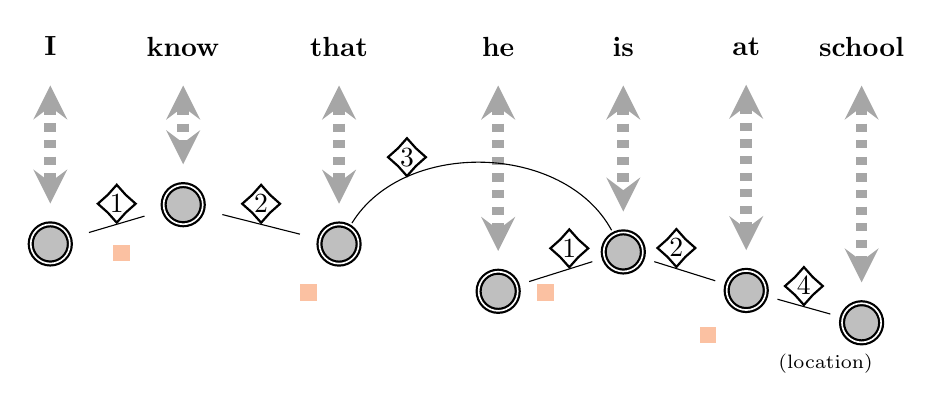
\begin{tikzpicture}

%\draw

%\node [s1] at (0,0) {Student};

\node (I) at (1,1) {\textbf{I}};
\node (know) [right=9mm of I] {\textbf{know}};
\node (that) [right=9mm of know] {\textbf{that}};
\node (he) [right=12mm of that] {\textbf{he}};
\node (is) [right=10mm of he] {\textbf{is}};
\node (at) [right=10mm of is] {\textbf{at}};
\node (school) [right=5mm of at] {\textbf{school}};


\node (IRep) [double,draw=black,shape=circle,thick,fill=gray!50,inner sep=.5em,below=2cm of I] {};
\node (knowRep) [double,draw=black,shape=circle,thick,fill=gray!50,inner sep=.5em,below=1.5cm of know] {};
\node (thatRep) [double,draw=black,shape=circle,thick,fill=gray!50,inner sep=.5em,below=2cm of that] {};
\node (heRep) [double,draw=black,shape=circle,thick,fill=gray!50,inner sep=.5em,below=2.6cm of he] {};
\node (isRep) [double,draw=black,shape=circle,thick,fill=gray!50,inner sep=.5em,below=2.1cm of is] {};
\node (atRep) [double,draw=black,shape=circle,thick,fill=gray!50,inner sep=.5em,below=2.6cm of at] {};
\node (schoolRep) [double,draw=black,shape=circle,thick,fill=gray!50,inner sep=.5em,below=3cm of school] {};

\node (knowRepType) [below right = .2cm and -1.2cm of knowRep] 
 {\colorbox{yellow!20!red!30}{\scalebox{.7}{\NNtoProp}}}; 

\node (thatType) [below right = .2cm and -.8cm of thatRep] 
{\colorbox{yellow!20!red!30}{\scalebox{.7}{\PropToN}}}; 

\node (isRepType) [below right = .1cm and -1.4cm of isRep] 
{\colorbox{yellow!20!red!30}{\scalebox{.7}{\NNtoProp}}}; 

\node (atRepType) [below right = .15cm and -.9cm of atRep] 
{\colorbox{yellow!20!red!30}{\scalebox{.7}{\NtoN}}
}; 

\node (atRepTypeNote) [below right = .5cm and .1cm of atRep] {
	\footnotesize{(location)}
}; 


\draw [ |-,-|, <->, line width = .8mm, draw=gray!70, 
 dashed, double equal sign distance, >= stealth, shorten <= .25cm, shorten >= .25cm ]
 (I) to (IRep);

\draw [ |-,-|, <->, line width = .8mm, draw=gray!70, 
 dashed, double equal sign distance, >= stealth, shorten <= .25cm, shorten >= .25cm ]
(know) to (knowRep);
 
\draw [ |-,-|, <->, line width = .8mm, draw=gray!70,  
 dashed, double equal sign distance, >= stealth, shorten <= .25cm, shorten >= .25cm ]
(that) to (thatRep);

\draw [ |-,-|, <->, line width = .8mm, draw=gray!70, 
 dashed, double equal sign distance, >= stealth, shorten <= .25cm, shorten >= .25cm ]
(he) to (heRep);
 
\draw [ |-,-|, <->, line width = .8mm, draw=gray!70, 
dashed, double equal sign distance, >= stealth, shorten <= .25cm, shorten >= .25cm ]
(is) to (isRep);

\draw [ |-,-|, <->, line width = .8mm, draw=gray!70,  
dashed, double equal sign distance, >= stealth, shorten <= .25cm, shorten >= .25cm ]
(at) to (atRep);

\draw [ |-,-|, <->, line width = .8mm, draw=gray!70, 
dashed, double equal sign distance, >= stealth, shorten <= .25cm, shorten >= .25cm ]
(school) to (schoolRep);
 
 
\draw [shorten <= .25cm, shorten >= .25cm ] 
(knowRep) to node [draw=black,shape = star,star points=4,thick,inner sep = 0mm, above] {1} (IRep);

\draw [shorten <= .25cm, shorten >= .25cm ] 
(knowRep) to node [draw=black,shape = star,star points=4,thick,inner sep = 0mm,above] {2} (thatRep);

\draw [shorten <= .05cm, shorten >= .05cm, bend left=60] 
(thatRep) to node [draw=black,shape = star,star points=4,thick,inner sep = 0mm,above, 
near start] {3} (isRep);


\draw [shorten <= .15cm, shorten >= .15cm ] 
(isRep) to node [draw=black,shape = star,star points=4,thick,inner sep = 0mm,
 above, pos=0.4] {1} (heRep);

\draw [shorten <= .15cm, shorten >= .15cm ] 
(isRep) to node [draw=black,shape = star,star points=4,thick,inner sep = 0mm,above, 
 pos=0.4] {2} (atRep);

\draw [shorten <= .15cm, shorten >= .15cm ] 
(atRep) to node [draw=black,shape = star,star points=4,thick,inner sep = 0mm,above] {4} (schoolRep);


%\draw [shorten <= .25cm, shorten >= .25cm ] 
%(s1Rep) to node [draw=black,shape = star,star points=4,thick,inner sep = 0mm, below] {2} (s2Rep);

%\draw [shorten <= .5cm, shorten >= .5cm ] 
%(afterRep) edge [bend left=20,looseness=1] node [draw=black,shape = star,star points=4,thick,inner sep = 0mm, 
% above, near end ] {3} (complainedRep);

%\node (frameTopLeft) [below left = 1.5cm and -.65 cm of s1] {};
%\node (frameBottomLeft) [below = 2.5cm of frameTopLeft] {};
%\node (frameBottomRight) [right = 3.95cm of frameBottomLeft] {};
%\node (frameTopRight) [above = 2.5cm of frameBottomRight] {};

%\draw [shorten <= 0.15cm, shorten >= 0.15cm ] 
%(frameTopLeft) edge [bend right=30,looseness=1] (frameBottomLeft);

%\draw [shorten <= 0.15cm, shorten >= 0.15cm ] 
%(frameBottomLeft) edge [bend right=30,looseness=1] (frameBottomRight);

%\draw [shorten <= 0.15cm, shorten >= 0.15cm ] 
%(frameBottomRight) edge [bend right=30,looseness=1] (frameTopRight);

%\draw [shorten <= 0.15cm, shorten >= 0.15cm ] 
%(frameTopRight) edge [bend right=30,looseness=1]
%node [draw=black,shape = regular polygon,regular polygon sides=3,thick,inner sep = .2mm, 
%above, near start, shape border rotate = 180] {4} (frameTopLeft);


%node [draw=black,shape = star,star points=4,thick,inner sep = 0mm, above, 
%bend left=100,looseness=3] {3}

%;


\end{tikzpicture}
\end{minipage}

\hspace{0.1\textwidth}
\begin{minipage}{0.8\textwidth}
		\renewcommand{\labelitemi}{$\blacklozenge$}
	
\begin{itemize}\setlength\itemsep{-.3em}
\item 1 \hspace{12pt}  Verb's subject argument
\item 2 \hspace{12pt}  Verb's direct object argument
\item 3 \hspace{12pt}  Propositional \q{packaging} (\q{typed} as {}\PropToN{})
\item 4 \hspace{12pt}  Locative auxiliary link \\
(may be typed as converting nouns to place-designations) 
\end{itemize}
\end{minipage}
\end{figure*}

\p{Incorporating 
type theory, we can skirt these issues by modeling phrases through the perspective of
type signatures: given Part of Speech annotations for phrasal units and then for
some of their parts, the signatures of other parts, like verbs or adjectives
linked to nouns, or adverbs linked to verbs, tend to follow automatically.  
A successful analysis yields a formal tree, where if (in an act of semantic
abstraction) words are replaced by their types, the \q{root} type is something like
\Prop{} and the rest of a tree is formally a reducible structure in
Typed Lambda Calculus: \NNtoProp{} \q{collapses} to \Prop{}, \ProptoN{} collapses
to \N{}, and so forth, with the tree \q{folding inward} like a
fan until only the root remains {\mdash} though a more subtle analysis would
replace the single \Prop{} type with variants that recognize different
forms of speech acts, like questions and commands.
In Figure ~\ref{fig:Iknow},
this can be seen via the type annotations: from right to left \NtoN{} yields the
\N{} as second argument for \i{is}, which in turn yields a \Prop{} that is mapped
(by \i{that}) to \N{}, finally becoming the second argument to \i{know}.  This calculation
only considers the most coarse-grained classification (noun, verb, proposition) {\mdash} as I
have emphasized, a purely formal reduction can introduce finer-grained grammatical or
lexico-semantic classes (like \i{at} needing an \q{argument} which is somehow an expression
of place {\mdash} or time, as in \i{at noon}).  Just as useful, however, may be analyses
which leave the formal type scaffolding at a very basic level and introduce
finer type or type-instance qualifications at a separate stage.}

\p{In either case, Parts of Speech are modeled as (somehow analogous to) 
functions, but the important
analogy is that they have \i{type signatures} which formally resemble functions'.
Words with function-like types proxy their corresponding phrase, not because 
they are necessarily more important or are Dependency \q{heads}, but 
because they supply the pivot in the type resolutions which, 
collectively/sequentially, progress to a propositional culmination.  
This epistemological telos induces a sequencing on the 
type resolutions {\mdash} there is a fixed way that trees collapse {\mdash} 
which motivates the selection of function-words to proxy phrases; 
they are not semantically more consequential, necessarily, but 
are landmarks in a dynamic figured syntactically as \q{folding inward}
and semantically as a progressive signifying refinement.   
Phrases are modeled via a \q{function-like} Parts of Speech along with one or more
additional words whose own types match its signature; the type calculations
\q{collapsing} these phrases can mimic semantic simplifications
like \i{many students} to \i{students}, but here the theory is explicit
that the simplification is grammatic and not semantic: the collapse
is acknowledged at the level of \i{types}, not \i{meanings}.  In addition,
tree structures can be modeled purely in terms of inter-word relations 
{\mdash} as I have proposed here with double-indices {\mdash} 
so a type-summary of a sentence's phrase structure can be notated and
analyzed without leaving the Link or Dependency Grammar paradigm.}

\p{In sum, then, function-like words can always be represented as 
the \q{head} of corresponding phrases, but this implies 
neither greater semantic importance nor that phrases are 
conceptual units that fully subsume their parts.  Instead, 
a \q{head-function} notation captures the idea that 
sentence-synthesis is bounded by considerations of 
conceptual integrity that we can model, to some coarse 
approximation, via type theory.  Designating \i{after} as 
the \q{head} in \i{student after student} means that we have a 
type machinery that models (coarsely but formally) how successive cognitive refinement 
converges onto something with the conceptual profile of a 
proposition, and that we can leverage this formality by 
identifying certain words as functional pivots in the 
synthesis-toward-proposition: these words are not necessarily 
pivotal in term of meaning, but they are the core skeleton of
the schematic type-based model which we attach to a 
sentence while modeling the constraints on its synthesizing 
process.  (There is a further dimension in the \i{student after student}
phrase {\mdash} the repetition of \q{student} {\mdash} which I will discuss later.)}

\p{Or at least, this is one area of analysis where type theory 
is relevant for linguistics.  I will argue that there are 
several different methodologies where linguists have 
turned to type theory, and moreover that they can 
be integrated into a unified picture organized around 
the granularity of types themselves, according to the 
relevant theories.}

\spsubsectiontwoline{Three tiers of linguistic type theory}

\p{When explaining grammaticality as type-checking {\mdash} the 
concordance between function-like signatures and 
word or phrase \q{arguments} {\mdash} types are 
essentially structural artifacts; their 
significance lies in the compositional patterns 
guiding phrases to merge into larger phrases in a 
well-ordered way {\mdash} specifically, that the \q{outermost}
expression, canonically the whole sentence, is 
type-theoretically a proposition.  I proposed earlier that 
sentence-understanding be read as an accretion of detail 
culminating in a complete idea; type-checking then imposes 
regulatory guidelines on this accretion, with each 
constituent phrase being an intermediate stage.  Assigning 
types to phrases presents a formal means of checking that 
the accretion stays on track to an epistemological 
telos {\mdash} that the accumulated detail will eventually 
cohere into a propositional whole, a trajectory formally 
captured by the progressive folding-inward of phrase types 
to a propositional root.}

\p{Types themselves are therefore partly structural fiats 
{\mdash} they are marks on intermediate processing stages 
embodying the paradigm that type-checking \i{captures}
the orderliness of how successive cognitive transforms 
accrue detail toward a propositionally free-standing end-point.  
At the same time, types also have semantic interpretations; 
the \N{}/\Prop{} distinction, for example, is motivated by 
the cognitive difference between nominals and states of affairs 
as units of reason.  Type-theoretic semantics allows the 
structural paradigm of type-checked resolutions, the 
tree \q{folding inward} onto its root, to be merged with 
a more semantic or conceptual analysis of types qua 
categories or classifications of meanings (or of 
units comprising meanings).  I have described this merger 
at a coarse level of classification, taking broad 
parts of speech as individual types, but similar 
methods apply to more fine-grained analysis.
By three \q{tiers} of linguistic organization, I am thinking of
different levels of granularity, distinguished by relative scales of
resolution, amongst the semantic implications of
putative type representations for linguistic phenomena.}

\p{From one perspective, grammar is just a
most top-level semantics, the primordial Ontological division of language into designations of
things or substances (nouns), events or processes (verbs), qualities and attributes (adjectives),
and so forth.  Further distinctions like count, mass, and plural nouns add
semantic precision but arguably remain in the orbit of grammar (singular/plural
agreement rules, for example); the question is whether semantic detail gets
increasingly fine-grained and somewhere therein lies a \q{boundary} between syntax and
semantics.  The mass/count distinction is perhaps a topic in grammar more so than
semantics, because its primary manifestation in language is via agreement
(\i{some} wine in a glass; \i{a} wine that won a prize; \i{many} wines
from Bordeaux).  But what about distinctions between natural and constructed objects,
or animate and inanimate kinds, or social institutions and natural
systems, matters more of grammar or of lexicon?}

\p{For example, the template \i{I believed
X} generally requires that \i{X} be a noun
(\qmarkdubious{}\i{I believed run}), but more narrowly a
certain \i{type} of noun, something that can be interpreted
as an idea or proposition of some kind (\qmarkdubious{}\i{I believed flower}).
Asher and Pustejovsky point out the anomaly in a sentence
like \q{Bob's idea weighs five pounds}
\cite[example 2, p. 5]{AsherPustejovsky}, which
possesses a flavor of unacceptability that feels akin to
Part of Speech errors but are not in fact syntactic
errors.  The object of \i{weigh} is \q{five pounds} and
its subject is \q{Bob's idea}, which is admissible
\i{syntactically} but fails to honor our semantic convention
that the verb \q{to weigh} should be applied to things
with physical mass (at least if the direct object denotes a quantity;
contrast with \i{Let's all weigh Bob's idea}, where the
\i{idea} is object rather than subject).  These conventions are
analogous to Part of Speech rules but more fine-grained:
there is a meaning of \i{weigh} which has (like any transitive
verb) to be paired with a subject and object noun, but beyond
just being nouns the subject must be a physical body
(in effect a sub-type of nouns) and the object a quantitative
expression (another sub-type of nouns).  Potentially, type
restrictions on a coarse scale (e.g. that the subject of a verb
must be a noun) and those on a finer scale (as in this
sense of \i{to weigh}) can be unified into an overarching theory,
which spans both grammar and semantics {\mdash} for instance,
both Part of Speech rules and usage conventions of the
kind often subtly or cleverly subverted in metaphor and
idioms (see \i{flowers want sunshine}, \i{my computer died},
\i{neutrinos are sneaky}, as rather elegantly compactified
by assigning sentient states to inert things).  This is one way of
reading the type-theoretic semantic project.}

\p{Certainly \q{Ontological} qualities of signifieds engender
agreements and propriety which appear similar to
grammatic rules. \i{The tree wants to run away from the dog} sounds wrong {\mdash} because
the verb \i{want}, suggestive of propositional attitudes, seems incompatible with
the nonsentient \i{tree}.  Structurally, the problem with this sentence seems analogous
to the flawed \i{The trees wants to run away}: the latter has incorrect singular/plural linkage,
the former has incorrect sentient/nonsentient linkage, so to speak.  But does this
structural resemblance imply that singular/plural is as much part of semantics as grammar, or
sentient/nonsentient as much part of grammar as semantics?  It is true that there are no
morphological markers for \q{sentience} or its absence, at least in English {\mdash} except
perhaps for \q{it} vs. \q{him/her} {\mdash} but is this an accident of English or revealing
something deeper?}

\p{In effect, assessments of propriety seem to operate on several levels.  First 
(not to imply an actual temporal priority, though) 
we may consider fine-grained word-sense: which lexical entrant for 
such-and-such word is plausible in the current context?  Then 
we can consider larger-scale Ontological criteria: is the subject 
of this sentence figured as material or immaterial, 
sentient or nonsentient, natural or sociocultural, spatially and/or 
temporally extended or pointwise; and so forth?  And finally, 
what Part of Speech is consistent for various words given syntactic
principles and morphological cues {\mdash} distinguishing noun/verb/adjective, 
and etc., along with singular/plural, mass/count, verb tense and case, 
and other criteria of morphosyntactic fit?}

\p{So type-related observations can be grouped (not necessarily
exclusively or exhaustively) into those I will call
\i{macrotypes} {\mdash} relating mostly to Parts of Speech and the functional treatment
of phrases as applicative structures; \i{mesotypes} {\mdash} engaged with
existential/experiential qualities and \q{Ontological} classifications
like sentient/nonsentient, rigid/nonrigid, and
others I have discussed; and \i{microtypes} {\mdash} related to lexemes and word-senses.
This lexical level can include \q{microclassification}, or
gathering nouns and verbs by the auxiliary prepositions they allow and
constructions they participate in (such as, different cases), and
especially how through this they compel various spatial and
force-dynamic readings; their morphosyntactic resources for describing states
of affairs; and, within semantics, when we look toward even more fine-grained classifications
of particular word-senses, to reason through contrasts in usage.\footnote{So, conceiving microclasses similar in spirit to Steven Pinker in
Chapter 2 of \cite{Pinker}, though I'm not committing to using the
term only in the way Pinker uses it.  Cf. also \cite{AnneVilnat}, which
combines a microclass theory I find reminiscent of \i{The Stuff of Thought} with
formal strategies like Unification Grammar.} Microclasses can point out similarities
in mental \q{pictures} that explain words' similar behaviors, or
study why different senses of one word succeed or fail to be acceptable in particular phrases.
There are \i{stains all over the tablecloth} and \i{paint splattered all over the tablecloth},
but not (or not as readily) \i{dishes all over the tablecloth}.  While \q{stains} is count-plural and
\q{paint} is mass-aggregate, they work in similar phrase-structures because both
imply extended but not rigid spatial presence; whereas \q{dishes} can work for
this schema only by mentally adjusting to that perspective, spatial construal shifting
from visual/perceptual to practical/operational (we might think of dishes \q{all over} the
tablecloth if we have the chore of clearing them).  Such observations support
microclassification of nouns (and verbs, etc.) via Ontological and
spatial/dynamic/configuration criteria.}

\p{Type-theoretic semantics can also apply Ontological tropes to unpack the overlapping mesh of word-senses,
like \i{material object} or \i{place} or \i{institution}.
This mode of analysis is especially well illustrated when competing senses
collide in the same sentence.  Slightly modifying two examples:\footnote{

\cite[p. 40]{ChatzikyriakidisLuo} (former) and
\cite[p. 4]{MeryMootRetore} (latter).}

\begin{sentenceList}

\sentenceItem{} \swl{}{The newspaper you are reading is being sued.}{lex}
\sentenceItem{} \swl{itm:Liverpool}{Liverpool, an important harbor, built new docks.}{lex}
\end{sentenceList}

Both have a mid-sentence shift between senses, which is analyzed
in terms of \q{type coercions} (see also \cite{ZhaohuiLuo}
and \cite{ZhaohuiLuoSignatures}).
The interesting detail of this treatment
is how it correctly predicts that such coercions are not guaranteed to
be accepted:

\begin{sentenceList}

\sentenceItem{} \swl{}{The newspaper fired a reporter and fell off
the table.}[(?)]{lex}
\sentenceItem{} \swl{}{Liverpool beat Tottenham and built new docks.}[(?)]{lex}
\end{sentenceList}

(again, slightly modifying the counter-examples).  Type coercions are
\i{possible} but not \i{inevitable}.  Some word-senses \q{block} certain coercions
{\mdash} that is, certain sense combinations, or juxtapositions, are disallowed.
These preliminary, motivating analyses carry to more
complex and higher-scale types, like plurals (the plural of a type-coercion
works as a type-coercion of the plural, so to speak).
As it becomes structurally established that type rules at the
simpler levels have correspondents at more complex levels, the use of
type notions \i{per se} (rather than just \q{word senses} or other
classifications) becomes more well-motivated.}

\p{Clearly, for example,
only certain kinds of agents may have beliefs or desires, so
attributing mental states forces us to conceive of their referents
in those terms:

\begin{sentenceList}

\sentenceItem{} \swl{}{Liverpool wants to sign a left-footed striker.}{ont}
\sentenceItem{} \swl{}{That newspaper plans to fire its editorial staff.}{ont}
\end{sentenceList}

This \i{can} be analyzed as \q{type coercions}; but the type-theoretic machinery should contribute
more than just obliquely stating linguistic wisdom, such as
maintaining consistent conceptual frames or joining only suitably
related word senses.  The sense of \i{sign} as in \q{employ to play on
a sports team} can only be linked to a sense of Liverpool as the
Football Club; or \i{fire} as in
\q{relieve from duty} is only compatible with newspapers as
institutions.  These dicta can be expressed in multiple ways.
But the propagation of classifications
(like \q{inanimate objects} compared to
\q{mental agents}) through complex type structures lends credence to the
notion that type-theoretic perspectives are more than just an expository tool;
they provide an analytic framework which integrates grammar and semantics, and
various scales of linguistic structuration.
For instance, we are prepared to accept some examples of dual-framing
or frame-switching, like thinking of a newspaper as a physical object and a city government
(but we reject other cases, like \i{Liverpool voted in a new city government and signed a
new striker} {\mdash} purporting to switch from the city to the Football Club).  The rules for
such juxtapositions appear to reveal a system of types with some parallels to
those in formal settings, like computer languages.}

\p{In short, \q{Ontological} types like \i{institution} or \i{place} serve in some
examples to partition senses of one multi-faceted word.  Here they reveal
similar cognitive dynamics to reframing-examples like \i{to the press}, where
Ontological criteria (like reading something as a place) are triggered by
phrase-scale structure.  But there are also interesting contrasts:
the \i{newspaper} and \i{Liverpool} examples
imply that some words have multiple framings which are well-conventionalized;
newspaper-as-institution feels less idiomatic and metaphorical than
press-as-place.  So these examples suggest two \q{axes} of variation.
First, whether the proper Ontological framing follows from other word-choices
(like \q{fire} in \i{the newspaper fired the reporter}, which has
its own semantic needs), or from morphosyntax
(like the locative in \i{to the press}); and, second, whether triggered framings work
by selecting from established word senses or by something more metaphorical.
Metaphors like \i{to the press} do have an element of standardization;
but apparently not so much so to be distinct senses: note how \i{the press} as metaphorical place
does not work in general: \qmarkdubious{}\i{at the press}, \qmarkdubious{}\i{near the press}
(but \i{at the newspaper}, \i{near the newspaper}
{\mdash} imagine two journalists meeting outside the paper's offices {\mdash} sound quite reasonable).}

\p{The \q{type coercion} analysis works for mid-sentence frame-shifts; but other
examples suggest a more gradual conceptual \q{blending}.  For example, the
place/institution dynamic is particularly significant for \i{restaurant}
(whose spatial location is, more so, an intrinsic part of its
identity).  Being a \i{place} implies both location and extension; most places are not single
points but have an inside where particular kinds of things happen.  I am not convinced
that restaurant as place and as institution are separate word senses; perhaps, instead,
conversations can emphasize one aspect or another, non-exclusively.  
We need not incorporate all framing effects via \q{subtypes} (restaurant as either
subtype of hypothetical \q{types of all} places or institutions, respectively).  But
\q{placehood}, the Ontological quality of being a place {\mdash} or analogously being
a social institution {\mdash} identify associations that factor into cognitive frames; types
can then be augmented with criteria of tolerating or requiring one association or another.
So if \q{restaurant} is a type, one of its properties is an institutionality that \i{may}
be associated with its instances.  In conversation,
a restaurant may be talked about as a business or community, foregrounding this
dimension.  Or (like in asking for directions) its spatial dimension may be foregrounded.
The availability of these foregroundings is a feature of a hypothetical restaurant type,
whether or not these phenomena are modeled by subtyping or something more sophisticated.
The \q{newspaper} examples suggest how Ontological considerations
clearly partition distinct senses marked by properties like objecthood or
institutionality (respectively).  For \q{newspaper} the dimensions are less available for
foregrounding from a blended construal, than \q{unblended} by conventional usage; that
is why reframings evince a type \i{coercion} and not a gentler shift of emphasis.
The example of \i{restaurant}, in contrast, shows that competing routes for
cognitive framing need not solidify into competing senses, though they trace
various paths which dialogs may follow.
But both kinds of examples put into evidence an underlying
cognitive-Ontological dynamic which has potential type-oriented models.}

\p{At the most general level {\mdash} what I called \i{macrotype} modeling {\mdash} a type
system recognizes initially only the grammatical backbone of expressions, and
then further type nuances can be seen as shadings and interpretations which add substance
to the syntactic form.  So in type-theoretical analysis at this more grammatic level,
we can still keep the more fine-grained theory in mind:
the relation of syntax to semantics is like the relation of a spine to its flesh,
which is a somewhat different paradigm than treating syntax as a logical or temporal
stage of processing.  Instead of a step-by-step algorithm where grammatical parsing
is followed by semantic interpretation, the syntax/semantics interface can be seen
as more analogous to stimulus-and-response: observation that a certain grammatic
configuration appears to hold, in the present language artifact, triggers a marshaling
of conceptual and cognitive resources so that the syntactic backbone can be filled in.
Perhaps a useful metaphor is grammar as gravitation, or the structure of a gravitational
field, and semantics is like the accretion of matter through the interplay of multiple
gravitational centers and orbits.  For this analogy, imagine typed lambda
reductions like \PropToNYieldsN{} taking the place of gravitational equations;
and sentences' grammatic spine taking the place of curvature pulling mass into a planetary center.}

\p{As I have argued, sentences' progression toward complete ideas can be 
assessed more semantically {\mdash} accretion of conceptual detail {\mdash} 
or more syntactically, in terms of regulated type resolutions pulling in 
from a tree's leaves to its root.  The latter model is a kind of 
schematic outline of the former, marking signposts in the accretion 
process rather like a meetings' agenda.  Type theory allows points in 
conceptual accretion to be selected {\mdash} corresponding to nested phrases 
{\mdash} where type-checking signals that the accretion is progressing 
in an orderly fashion.  Or, more precisely, type-checking acts 
as a window on a cognitive process; phrasal units are like 
periodic gaps in a construction wall allowing us to reconstruct interpretive 
processes, and the possibility of certain linguistic elements being 
assigned types marks the points where such windows are possible.  
So type theory can impose a formal paradigm on our assessment 
of sentence structure, but at the cost of sampling only 
discrete steps of an unfolding completion toward understanding.  
In practice, this discrete analysis should be supplemented 
with a more holistic and interpretive paradigm, which explores 
{\mdash} perhaps speculatively, without demanding thorough 
formalization {\mdash} the gaps between the formalizable windows.  
I will transition toward this style of analysis in the next section.}

\thindecoline{}
\p{At the same time, I feel that the foundations of \q{cognitive}
linguistics deserve a little more attention.  I have used
\i{cognitive} rather informally, depending on the intuitive 
picture of \q{cognitive} linguistics, grammar, or indeed
\q{cognitive phenomenology}, which emerges from the 
speculative project we associate with linguists/philosophers 
like George Lakoff, Mark Johnson, Leonard Talmy, 
Ronald Langacker, and Peter \Gardenfors{} {\mdash} along with, as
\Gardenfors{} points out, phenomenologists like Jean Petitot.\footnote{ \Gardenfors{} mentions Lakoff, Langacker, Talmy, Fauconnier, 
and others alongside \q{a French semiotic tradition, 
exemplified by [Jean-Pierre] Descl\'es ... and 
[Jean] Petitot-Cocorda ... which shares many features with the 
American (mainly Californian) group} \cite[p. 4]{Gardenfors}.} At the same time, Petitot also links with a 
tradition that combines elements of phenomenology and 
Analytic Philosophy, represented by philosophers like 
Barry Smith and David Woodruff Smith and by \q{Analytic Phenomenology}
or \q{Naturalizing Phenomenology} projects, the latter also being 
a large volumes Petitot co-edited.\footnote{Petitot's and Barry Smith's formalizing projects were parallel
and collaborative to some extent.  Maxwell James Ramstead
in a 2015 master's thesis reviews the history elegantly:

\begin{quote}
Now, the \q{science of salience}
proposed by Petitot and Smith (1997) illustrates the
kind of formalized analysis made possible through the direct
mathematization of phenomenological descriptions.
Its aim is to account for the invariant descriptive
structures of lived experience (what Husserl called \q{essences})
through formalization, providing a descriptive geometry of
macroscopic phenomena, a \q{morphological eidetics} of the
disclosure of objects in conscious experience (in Husserl's
words, the \q{constitution} of objects).
Petitot employs differential geometry and morphodynamics
to model phenomenal experience, and Smith uses formal structures from
mereotopology (the theory of parts, wholes, and their boundaries)
to a similar effect. \cite[p. 38]{Ramstead}
\end{quote}
}
\q{Cognitive} in these contexts 
tends to imply desire to ground analyses on holistic
human experience, in its experiential, embodied, pragmatically-oriented, 
first-personal, and intersubjective dimensions.\footnote{Note that in this sense
\q{Cognitive} connotes a very different perspective than this same 
term in \AI{} research, for example; on the one side we have a 
philosophical commitment to the irreducibility of
human reason to computable \q{symbol processing}, whereas 
on the other there is a paradigm where, in effect 
(perhaps simply because mental activity is presumably 
reducible to low-level biological processes), there 
exists \i{some} computable core of cognition, which scientists 
can unlock to build powerful \q{Artificial General Intelligence}.}
}

\p{Cognitive linguistics can be called \q{speculative} because its 
methodology generally relies on linguists' assessments of 
acceptability rather than empirical data from surveys, 
computational or statistical analyses of copora, or 
psycholinguistic studies of language processing or acquisition.  
Analytic Phenomenology is speculative in similar ways; 
although in some cases phenomenological structures are 
related to formal/mathematical theories like 
Mereotopology or Differential Geometry (cf. Barry Smith and 
Petitot, respectively, or Kit Fine's \i{Part-whole}
\cite{KitFine}), phenomenologists' assessments of 
common perceptual patterns (and how they are 
situationally or conceptually interpreted and engaged with) 
is principally introspective.  Both phenomenologists 
and cognitive linguists, in short, introspect on 
conscious and linguistic experience to identify patterns 
which they believe are not eccentric to their own cognition,
but have some public disputability and theoretical merit.  
Of course, the overall dialog wherein philosophers debate 
and compare their own introspective reports allows 
this speculative method to have some rigor, because descriptions 
of cognitive processes {\mdash} in their first-personal 
facticity {\mdash} which seem both subjectively faithful and
structurally revealing will emerge as analyses of 
general pattern so long as multiple philosophical treatments 
agree on their fidelity to experience.  So 
analyses get theoretically favored if they meet three 
different criteria of structural productivity {\mdash} in the 
sense that produce new insight onto cognitive processes, 
rather than just describing cognition as an experienced
givenness {\mdash} plus both faithfulness to each person's 
conscious experience and also generality to many 
people's experience.\footnote{So for instance, Husserl's examination of 
protention and retention in sensing spatial form during 
perceptual episodes focused on discrete, extended objects 
(e.g. in \i{Thing and Space}), or his investigation of 
how intersubjectivity contributed to consolidating our 
conceptual integration of perceptual givens 
(e.g. in the \i{Cartesian Meditations}), can be 
considered classic phenomenological analyses because they 
have been deemed both experientially accurate and 
theoretically insightful by subsequent generations' worth of 
public review.}
}

\p{At their best, then, both phenomenology and cognitive linguistics 
combine introspective analysis and public disputation to 
develop theories of cognitive-experiential structures {\mdash} of 
how the immediate structuraion of perceptual experience as 
primordial conscious content unfolds into the
schematic and rational models of our surrounding environment
and situations, for purpose of goal-directed activity and 
inter-personal, collective reasonableness.  The underlying assumption 
is that raw structures, below the threshold of conscious 
deliberation, are enmeshed in immediate experience, and that from 
there we can identify ambient and situational patterns; 
mental representations of 
the structural and material properties of surrounding 
objects and places and the social/pragmatic rules 
governing interpersonal situations.  We can then 
posit situational prototypes and morphological principles 
apparently operating in these representations, which become 
the basis of systematic theorizing of cognitive activity 
in general, including language.}

\p{In this paradigm, situational and organizational prototypes 
and patterns lend their structure to language, so 
{\mdash} in many cases, i.e., with respect to many 
language artifacts {\mdash} the scenarios influencing 
linguistic structure are these extra- or pre-linguistic 
gestalts rather than semantic to syntactic rules
\i{per se}.  But for this belief about the origin of 
(at least some) surface-level linguistic form to be 
leveraged as a diligent semantic or syntactic method, 
we need a systematic account of how phenomenological 
pattern evolve into (by grounding) linguistic 
structures.  A thorough treatment of this problem 
is far beyond the scope of one paper, but I will 
offer a few ideas in the remainder of this section.}

\subsection{Types and Phenomenology}
\p{In their proper context, understanding linguistic expressions 
requires binding language to objects or \q{phenomena} in 
speakers' collective perceptual (or conceptual) horizon.  
Referents are not always material things; they can even 
be the \i{absence} of objects, or of substance:

\begin{sentenceList}

\sentenceItem{} \swl{itm:footprints}{There are footprints on the beach.}{ref}
\sentenceItem{} \swl{itm:hole}{There's a hole in the bucket.}{ref}
\sentenceItem{} \swl{itm:footprintsleading}{There are footprints leading up the hill.}{ref}
\sentenceItem{} \swl{itm:traintracks}{There are train tracks leading up the hill.}{ref}
\end{sentenceList}

In (\ref{itm:footprints}) our attention is direct not to any \i{object}, but 
to a certain perceptual pattern which has some factual significance, enough 
to warrant a distinct concept.  Insofar as \i{one} footprint is a 
focus of attention, we notice some pattern of discontinuity which allows 
a foreground to emerge from a background {\mdash} but there is perceptual 
blend of discontinuity and continuity, since a footprint is literally 
situated in a material expanse with its surroundings.  To focus on the 
footprint {\mdash} a cognitive act which is both perceptual and conceptual 
{\mdash} we have to retain awareness both of the footprint materially 
continuous with the surrounding sand (say) and also distinct from it 
via a somewhat different color or composition (e.g., the sand in the footprint 
may be darker or more compact than the sand around it).  When talking 
about \i{footprints}, plural, we have to direct attention to a perceptual 
totality, something extending over our visual field and possessing inner 
parts, but also suggesting a conceptual totality, a worthiness of 
being cognized in aggregate.}

\p{In (\ref{itm:footprintsleading}), moreover, we conceive the totality in conjunction 
with a sense of direction, and protention.  The implication is that we 
do not see \i{all} of the footprints, but we can discern from their 
pattern a direction which, we anticipate, will reveal more footprints.  
Meanwhile the footprints are presumably disjoint, unlike train tracks.
So the perceptual foreground in (\ref{itm:footprintsleading}) is phenomenologically 
complex, including a totality we perceive that implies a greater 
totality, part of which is experienced anticipatorily rather than 
explicitly, along with a fragmentation which nonetheless permits a 
perceptual unification into a coherent whole.  These kinds of 
perceptual/conceptual complexities in arrangements 
{\mdash} blending continuity and discontinuity, wholeness and 
fragmentation, sensation and protention {\mdash} are canonical 
to the phenomenology of attentional foci in any cognition 
engaged with ambient situations, which certainly 
includes language.  We are not robots experiencing the 
world as a tableau of simply discrete, integral object-\q{things}.}

\p{Language serves as a guide to negotiating the complexities of 
perceptual foci in inter-personal environments.  
We therefore have to understand how language
\q{hooks} into conversants' phenomenological faculties. 
So we have, at a basic level, a 
contrast between situationally grounded or conceptually 
generalized references:

\begin{sentenceList}

\sentenceItem{} \swl{itm:Salesmen}{Salesmen are intelligent.}{ont}
\sentenceItem{} \swl{itm:knocking}{Salesmen are knocking on the door.}{ont}
\sentenceItem{} \swl{itm:Should}{Should I let them in?}{ont}
\end{sentenceList}

The effects of (\ref{itm:knocking}) 
(which with (\ref{itm:Salesmen}) are from the \i{Handbook}, example 44, page 169, 
chapter 6) are manifest in several 
changes to conversants' collective understanding: (\ref{itm:knocking}) 
establishes both a domain of potential reference (the salesmen 
could be subsequently identified as \i{the salesmen} or
\i{those salesmen} or \i{them}), and the fact of their being 
at the door established as a basis for further dialog (e.g., 
(\ref{itm:Should})).  The more generic (\ref{itm:Salesmen}) 
does not have any comparable situational effects, though 
it permits further dialog on a more generic plane.}

\p{Sometimes, of course, people dialog about things that are 
perceptually evident around them collectively.  Probably 
more common, though, is that the structures of 
presentational perception translated to general 
cognitive patterns that are signified through language.  
That is to say, the rules of perceptual gestalts 
{\mdash} the partial continuity and partial discontinuity 
between background and foreground; and the mixture of 
singular integrity and divisibility characterizing attentional  
foregrounds {\mdash} are taken for granted as patterns 
typifying perception in general, whether that be 
perceptions presently occurring in the situational 
context or those conceptualized indirectly, abstractly, 
or hypothetically.  How foci of attention figure into 
perceptual continua become part of their extralinguistic 
background, reflected in lexical conventions:

\begin{sentenceList}

\sentenceItem{} \swl{itm:ink}{There are ink stains on the pages of this book.}{ref}
\sentenceItem{} \swl{itm:sunset}{There is a pretty sunset over the river.}{ref}
\sentenceItem{} \swl{itm:cicada}{In some neighborhoods, cicada insects make loud sounds from sunset to sunrise.}{ref}
\udref{en_gum-ud-train}{GUM_voyage_phoenix-30}
\sentenceItem{} \swl{itm:applause}{The audience rose to give thundering applause.}{ref}
\end{sentenceList}

The unifying theme in these examples is that their central concepts are 
experienced in terms of a matrix of phenomenological criteria that can 
be harnessed into a general theory: how an ink stain is (in part) 
materially continuous with the stained paper that extends around it; 
how \i{a pretty sunset} is an imprecisely bounded but conceptually 
integral atmospheric event; how (\ref{itm:applause}) figures the audience as 
discrete individuals who, at that moment, act in such a way as to present a 
conceptual and perceptual totality; how (\ref{itm:cicada}) likewise proposes 
a totality but in a more complex fashion, because the speaker is 
describing a typical \i{kind} of experience rather than the specific 
sounds of cicadas on one specific occasion.}

\p{The matrix of continuity/discontinuity, and individual coherence balanced
(within intentional \q{noemata}) 
against internal structuration and diversity, 
are \i{conceptually} intrinsic to notions like \i{ink stains} (or \i{footprints}),
\i{applause}, \i{sunsets}, and even \i{cicadas} and \i{noises}.  
They become part of a language's lexical machinery and 
therefore embed, in lexical conventions, phenomenological 
prototypes that imply a situational background, called 
forth by the lexical potency of the specific words.  
The point is not that the hearer of (\ref{itm:sunset}), say, 
sees the sunset also, and thus \i{explicitly} undergoes the 
disclosure-experience of a sunset (in all its sensory 
vividness and individuating vagueness).  Instead, the 
patterns of sensation and (dynamic, imprecise, un-fixed) 
individuation are abstracted to prototypes poised within 
the lexicon itself to be perceived as applicable to the 
talked-about situation.  We have some idea of the
\i{kind} of experience is involved in a sunset, not just 
perceptually but in the nexus of conceptual and 
rational processes which leads us to identify the sunset 
as such and estimate its phenomenal specificity 
{\mdash} its spatial form, its temporality {\mdash} so that it 
has some determinate epistemic content, something 
that can be discussed with others (\i{Did you see the 
sunset}; \i{Is it too late to see the sunset}; etc.).}

\p{Phenomenological patterns in construing conceptual and 
referential foci, solicited by lexical and idiomatic 
conventions, give language flexibility and rhetorical 
flair, often bounding expressive possibilities on 
phenomenological rather than narrowly semantic grounds.  
I would dispute some of Nunberg's analyses I mentioned 
in the last section, for example, on the 
dubiousness of (\ref{itm:start}) or the exceptionality 
of (\ref{itm:Sauternes}).  I do not find
(\ref{itm:start}) exceptionally jarring, considering the 
situational construal common to (\ref{itm:start}) along 
with (\ref{itm:parked}) and (\ref{itm:waiting}): 
the formation \i{I am parked} is not \i{just} a matter of 
a person proxy-referring their car.  Usually a person 
saying \i{I am parked} is \i{in} their car, so they are 
describing a larger situation {\mdash} the conceptual foreground 
is the totality of the car and themselves in it.  Were the 
addressee to find them, their attention would be directed 
to the car \i{and} the speaker, as a complex but 
integral (in that episode of time) whole.  
This then carries over to cases where the speaker 
is \i{not} in their car.  Saying \i{I am parked} (along with 
a place-description) outlines the steps needed to return to 
the car; it is a way of framing the car's location 
operationally.  Using the first person for where the car is 
parked {\mdash} even when the speaker is not at that spot 
{\mdash} indicates that the speaker is conceiving the car's 
location in first-personal terms; that is, in terms 
of the actions the speaker is taking or anticipates 
taking.}

\p{This analysis then implies that (\ref{itm:start}) is 
acceptable on similar operational grounds; first-personalizing 
the cars location, so to speak, foregrounds that location 
only in the context of an operational totality involving 
(presumably) going to the car and then driving it.  
If the speaker is concerned about the car not starting, 
this is relevant to how the overall situation is 
cognized, and therefore the transition from the speaker-centered
\i{I am parked ...} to the discordant \i{and may not start}
is understandable.  I would similarly argue that the 
apparent difference between (\ref{itm:Sauternes}) and
(\ref{itm:beers})-(\ref{itm:Michelobs}) depends on how 
referential foci are established.  The phrase
\i{a beer} can designate a specific glass or bottle of 
beer {\mdash} something perceptually and enactively/kinaesthetically 
individuated {\mdash} or also a specific preparation of beer,
individuated by the unique flavor of the beverage rather than 
the material identity of the liquid.  These 
differences have phenomenological overtones: if I say
\i{I drank two beers} I could mean two glasses, pints, or 
bottles; I could also mean two \i{kinds} of beer 
(maybe multiple pints of each).  The phrasing itself 
is ambiguous, but the ambiguity is extra-linguistic: 
it relates to how linguistic content binds to empirical 
givens with their rules of phenomenological 
individuation.  The \q{two pints} reading implies 
one kind of phenomenological architecture governing
\q{word-to-world fit}, where elements in language 
link to discrete, perceptually/operationally integral
objects like glasses (though of course a glass of 
beer is also an integral complex where the beer and 
the glass are semi-autonomous parts).  The \q{two kinds}
reading is more subtle, resting conceptual focus on the 
belief that a distinct kind of beer has a distinct 
flavor that is both unique \visavis{} other beers and 
also consistent across bottles (or kegs), so it has
\i{a} taste that people can jointly experience and 
talk about.  Nunberg makes the reasonable claim 
that we are more likely the hear the 
former interpretation when it comes to beers, and 
the latter one for Sauternes, but I can imagine plausible
conversations where these conventions would be reversed.}

\p{To return to type theory, then, this style of 
formalization is a potential window onto how the 
lexicalized concepts negotiate the phenomenological 
options in \q{binding} words to phenomena.  
The matrix of continuity/discontinuity and 
individuation (singularity)/complexity (internal 
structure or diversity) forms a tableau which 
different word senses and, in explicit phrase contexts, 
different usages \q{hook into} in different ways.  
So beer \i{qua} liquid has one conventional 
pattern in \q{word-to-world fit}, while beer
\i{qua} consumer product, or a brewer's creative 
endeavor, evinces a different phenomenological 
pattern.  This is modeled, to some approximation, 
by the \q{type} (or as I put it \q{mesotype}) 
distinction of a liquid (more generally a substance) 
against a consumer product or social good 
(more generally a socio-cultural artifact).  We 
can refer to beers in both senses, and I have 
mentioned theories of type \q{coercions} or
juxtapositions (cf. Pustejovsky's \q{dot product}
theories in \cite{JamesPustejovsky} or
\cite{AsherPustejovsky}) that explore when 
the different \q{Ontological} construals or sentences can be 
combined or alternated.  At this point I would add that 
these Ontological details are not only relevant to 
semantics; they also govern how phenomenological 
patterns can be reified and typified in lexical and 
idiomatic conventions.}

\thindecoline{}

\p{For successful conversation, participants need to converge 
for each sentence on a common conceptual focus; not surprisingly, 
this process often reciprocates the phenomenology of 
perceptual focus, or enactive/kinaesthetic attention.  
Drawing form from phenomenological structure, referential 
signification often takes shapes that can seem opaque 
on purely logical considerations.  In analysis of 
referring expressions, then {\mdash} analogously to 
semantic analyses as earlier in this section {\mdash} we need 
to be sensitive to the possibilities of language form 
molding to perceptual and situational gestalts rather 
than predicate structure.}

\p{Nunberg, for instance, investigates how the proxying effect in
\i{I am in the Whitney} can be generalized to other cases.  
I'll point out that this fits a not-uncommon rhetorical 
pattern, as in:

\begin{sentenceList}

\sentenceItem{} \swl{itm:hall}{I am in the Hall of Fame.}{ref}
\sentenceItem{} \swl{itm:ontv}{I am on TV.}{ref}
\end{sentenceList}

Nunberg argues that reference, in these kinds of cases, will
\q{transfer} between conceptually
linked designata, so I can refer to my car's location as my location, 
or to my painting as myself.  If we analyze this logically, 
the rule appears to be that I can substitute first-person 
reference for reference to something associated with 
myself (that I own or have created, etc.).  
He then finds that the pattern does not generalize to a 
scenario such as a painter {\mdash} referring to the location of her
work in transit {\mdash} saying something like (his example 12):

\begin{sentenceList}

\sentenceItem{} \swl{itm:crate}{I'm in the second crate on the right.}{ref}
\end{sentenceList}

In other words, Nunberg's analysis turns on theorizing various
\q{I am in...} constructions as a kind of referential transfer 
or (as I would say) proxying, and then seeking the logical rules 
behind how and when such proxying works in a first-person
(morphosyntactic) context.\footnote{Obviously \q{first person} in this setting concerns
verb tense and other linguistic cues linking to
the speaker/enunciator of a piece of language; the
same term is also encountered (including elsewhere
in this paper) in the phenomenological
(and Philosophy-of-Mind) sense of
conscious, intentional experience (in contrast
to experience, or thoughts and feelings, we
attribute to others based on their behavior).}
}

\p{On the other hand, I would argue that the pattern in 
(\ref{itm:hall})-(\ref{itm:ontv}) is not reducible to 
referential proxying as a logical maxim.  We can speculate that
\i{I} obliquely references, say, the bust and info about an 
athlete who has been elected to a Hall of Fame, or to the 
image of a TV personality which viewers see on screen.  
So analyzing this construction as a case where reference 
is transferred from the \q{subject of enunciation} to 
some subordinate vehicle {\mdash} her bust, image, and so forth 
{\mdash} is a plausible gloss on the pattern.  But looking for a 
single maxim to accommodate these different cases overlooks 
the contextual particulars, in particular the backstory 
which is lexically embedded in expressions like
\i{Hall of Fame} and \i{on TV}.  There is a long process 
leading to retired athletes being recognized as worthy of 
a Hall; there is also a long process whereby personalities 
get a chance to appear on television.  Actually, (\ref{itm:ontv}) 
has two interpretations {\mdash} someone could be on TV just momentarily, 
e.g. as a bystander during on-location news coverage {\mdash} or 
as someone like a policy expert who is interviewed on occasion.  
But the more interesting reading of (\ref{itm:ontv}) involves 
a person being described as \q{on TV} not on the occasion of 
their appearing on-screen in that moment, but as a recurring 
event.  In this case \i{being on TV} encapsulates a backstory 
reflecting a measure of personal success and esteem, not unlike 
an athlete in a Hall of Fame or an artist in a prestigious museum.}

\p{The relevant backstories govern interpretations for first-person 
reference: \i{I am in the Hall} or \i{on TV} indirectly reports 
that the speaker has undergone some process which the addressee, 
assumed competent with the relevant lexicon, at least
minimally understands.
So a pattern like (\ref{itm:hall}) packages up that backstory
\i{in the guise} of a referring expression; it is not so much the 
athlete's bust as a target of referential proxying, but more of the 
act of referring to that bust (i.e., to the referentiable 
object manifesting the speaker's being elected) entering
the Hall of Fame backstory into the discursive ledger.  This 
carries over to the Whitney case: calling oneself
\q{in} a museum does not just proxy the self for one's art, 
but uses patterns of reference to the art work as a 
vehicle for introducing the backstory of one's 
rise through the art world (or whatever is the relevant 
autobiographical context) into the conversation.}

\p{I would argue, in short, that referential proxying is not a 
primarily logical operation, but relies on backstory context to 
regulate how referring patterns are received.  To establish conceptual 
foci, addressees have to negotiate the language given to them, in 
search of the focal element or foreground, often an explicit or 
hypothetical perceptual nexus.  So a painter \i{in the Whitney} means 
that a visitor can, in the right room and orientation, perceptually 
encounter her work; a personality \i{on TV} means that the 
addressee can, at times, see her on-screen.  Those potential perceptual 
givens ground the semantics of expressions like (\ref{itm:Whitney}) or 
(\ref{itm:ontv}).  This does not mean that the sentences are only 
meaningful to an addressee who wants to go find the speaker at the 
museum or on the television.  But it does present the perceptual 
ground as a foundation for the conceptual implications which 
lead from that perceptual situation: from the perceptual presence 
of an art work in a museum to the backstory of its provenance 
and implications for the artist's career or place in history; 
or from the on-screen image to the context of how TV shows 
are produced and the careers and reputations of the figures that 
show up.}

\p{We approach referring expressions in these contexts at two levels: 
we identify the canonical perceptually-oriented references which 
supply a conceptual ground (the painting as perceptual 
object, the on-screen image as perceptual simulacrum); but then 
we recognize the backstory and situational context which 
determines how the perceptual ground should be understood.  
Usually the discourse is \q{about} that backstory, not about 
the precise situations where explicit perceptual grounds would 
be relevant {\mdash} an artist probably would not say 
(\ref{itm:Whitney}) only to someone looking to visit a museum to 
see her art work.  The \q{I am in...} pattern 
turns on how these two different levels are played off 
in interpretation.
In particular, the addressee needs to ascertain why the
speaker's information is being proferred: is boasting
of their art being hung in an elite museum mostly a
way of conveying the speaker's status, so the main theme is
essentially autobiographical; or is the actual location
of the painting directly relevant to the present conversation?}

\p{A statement like (\ref{itm:crate}) (the speaker being
\q{in the crate on the right}) does not have the more
\q{autobiographical} reading, since (absent some bizarry
imaginary scene) there is no status or reputation attached
to which crate is carrying your paintings.  But the second kind of reading,
where specific location is operationally relevant,
is plausible in some contexts; perhaps several different
artists' works are in several different crates and
the speaker wants to direct focus onto the one holding
her own works.  So, in the proper context,
I have no objection to
(\ref{itm:crate}) or \i{I am in that crate} (forms which Nunberg rejects).
The gist here, as in (\ref{itm:Whitney}), is to establish conceptual
focus onto a painting or art work, and to do so via a
first-person referential lead-in.  So the situation determines 
first \i{why} the focus is thus singled out and second
\i{how} the first-person reference can proxy that focus.  
In (\ref{itm:Whitney}), we single out a painting insofar as it 
is a product of the artist's creativity, so appreciation of the 
work is manifestly appreciation of the artist.  The artist is 
then referentially linked to the work because the backstory of 
how museums acquire art works overlaps with the story of 
artists' careers and reputations.}

\p{In (\ref{itm:crate}) the situation is different: presumably 
the focus is on one or several art works because of some concern 
about transporting or accessing them, so we're attending to the 
works in their guise as (fragile) physical objects.  Moreover 
the link between the artist and the work, which guides the 
referential proxying, is presumably that the artist is 
concerned about accessing and protecting those objects.  
The situational elements are different, but in both these 
cases {\mdash} whether paintings are in the crate or in the 
Whitney {\mdash} there is some structural resonance in how
situational, backstory, and hypothetical-perceptual 
gestalts are all integrated into patterns of grounding 
referential interpretation in ambient conceptual contexts.}

\p{I think that linguists sometimes underestimate the 
multiplicity of layers {\mdash} situational, contextual, 
phenomenological (explicit and hypothetical), 
referential, contextual {\mdash} that all converge on 
meaning and reference.  Perhaps this tendency can
be empirically examined by testing judgments of
acceptability: the more that we incorporate
multiple layers of posssible context, the wider becomes
the circle of sentences that feel reasonable
(cf. the reasonableness, in my estimation, of
(\ref{itm:crate}) and (\ref{itm:Sauternes})).\footnote{Granted that, perhaps, with a lot of imagination
almost any construction could be deemed
plausible in \i{some} context.  Accordingly,
one could argue that it is analytically reasonable
to distinguish sentences that exemplify proper
language in a wide range of contexts, as compared
to sentences which could only be meaningful
in very select circumstances.  Even on this perspective,
however, we have to unpack the distinction between
\q{generic} from \q{select} circumstances {\mdash} what
qualities of these situations, together with
relevant word-meanings, make these examples
of broad usage patterns as against unexpected
usages that are nonsensical without a very
specific background?  Rather than being a neutral
arbiter of acceptability, such genericity is a
phenomenon that needs to be explained.  I would
argue that assessments of unacceptability will in
many cases overrate the distinction between
\q{normal} and \q{exceptional} circumstances.
For example, I dispute that the beer/wine
contrast, or painting in a museum or in a crate
contrast, are such a divergence between normal and
unusual contexts that (\ref{itm:crate}) has
essentially different plausibility than
(\ref{itm:Whitney}), or (\ref{itm:Sauternes})
compared to (\ref{itm:beers}) and (\ref{itm:Michelobs}).} Failure to identify these
layers' workings can lead analysis toward searches 
for reproducible logical rules governing which constructions  
are accepted by a language-community as recurring patterns, 
and logical explanations for the limits on that 
generalizability.  This is one example of
overestimating the logicality of language in 
general, an issue I have approached in this section 
from both semantic and reference-theoretic angles.  
I will focus on this issue of logicality {\mdash} both its applicability 
and its limits {\mdash} in the next section.}

\section{Gaps in Truth-Theoretic Semantics}
\label{s3}
\label{sec:Gaps}
\p{I take as a given that typical sentences have a propositional core, 
against which they take a performative stance 
(which can be outright assertion, or else asserting speakers' 
more complex propositional attitudes).  I would further 
say that \i{truth-theoretic} semantics, in particular, 
is organized around this propositional content as the 
core target of linguistic analysis.  I am thinking of 
truth-theoretic semantics in a broad sense, perhaps the 
most influential paradigm in the Philosophy of Language 
and by extension philosophy and linguistics in general 
(not to mention Computer Science and Artificial Intelligence 
research).  The most notable counter-paradigm is Cognitive Linguistics; 
consider George Lakoff and Mark Johnson's extended critique 
of truth-theoretic paradigms in \i{Philosophy in the Flesh}.  
Adherents of the latter perspective need not 
dispute the logical substance of language artifacts' propositional 
content, but tend to direct theoretical attention not to 
the nature of propositional content itself, but to the cognitive 
processes through which this content is understood.}

\p{As I argued earlier, many sentences do not simplistically 
reproduce the logical structure of their propositional 
content, so models of that structure are only tangentially 
relevant to analysis on the language side.  This is why we 
need distinct analyses, beyond a mere logical gloss, 
covering the interpretive steps leading to holistic 
sentence-understanding.   This section will consider several 
cognitive and pragmatic themes moving toward a general theory 
of this phenomenon.}

\subsection{Enaction and Illocutionary Force}

\p{I will start by reviewing illocutionary pragmatics, to 
identify some of the contextual and interpretive 
transformations that pertain to mapping surface language 
to propositional contents.  My point is to establish 
what should be a common theory of logicality that can be
shared by both critics and defenders of \q{truth-theoretic}
paradigms, on which basis their legitimate disputes 
can be investigated.}

\p{Many linguists (on both sides, I would say, of my 
central truth-theoretic pro/con), 
seem to analyze hedges like \q{could you please}
as merely dressing over crude commands: we don't
want to come across as giving people orders, but
sometimes we do intend to ask people to do specific
things.  As a result, we feel obliged to couch the
request in conversational gestures that signal
our awareness of how bald commands may lie outside
the conversational norms.  These ritualistic
\q{could you please}-like gestures may have
metalinguistic content, but {\mdash} so the theory
goes {\mdash} they do not \i{semantically} alter
the speech-act's directive nature.}

\p{The problem with this analysis is that sometimes
directive and \q{inquisitive} dimensions can
overlap:

\begin{sentenceList}

\sentenceItem{} \swl{itm:almond}{Do you have almond milk?}{pra}
\sentenceItem{} \swl{}{Can you get MsNBC on your TV?}{pra}
\sentenceItem{} \swl{itm:needcorkscrew}{This isn't a screw-cap bottle: I need a corkscrew.}{pra}
\end{sentenceList}

These \i{can} be read as bare directives, and would
be interpreted as such if the hearer believed the
speaker already knew that yes, he has almond milk, and yes,
he gets MsNBC.  In (\ref{itm:needcorkscrew}), if both parties
know there's one corkscrew in the house,
the statement implies a directive to fetch \i{that} corkscrew.
But, equally, (\ref{itm:almond})-(\ref{itm:needcorkscrew}) can \i{also} be read as bare
questions with no implicature: say, as fans of
almond milk and MsNBC endorsing those selections,
or pointing out that opening the bottle
will need \i{some} corkscrew.
And, meanwhile, (\ref{itm:almond})-(\ref{itm:needcorkscrew})
can \i{also} be read as a mixture of the
two, as if people expressed themselves like this:

\begin{sentenceList}

\sentenceItem{} \swl{}{I think the window is open, can you close it?}{pra}
\sentenceItem{} \swl{}{I see you have almond milk, can I have some?}{pra}
\sentenceItem{} \swl{}{If you get MsNBC, can you turn on Rachel Maddow?}{pra}
\sentenceItem{} \swl{}{If there is a corkscrew in the house, can you get it?}{pra}
\end{sentenceList}
}

\p{I think the mixed case is the most prototypical, and pure
directives or inquiries should be treated as degenerate
structures where either directive or inquisitive content
has dropped out.  After all, even a dictatorial
command includes the implicit assumption that the order
both makes sense and is not impossible.  On
the other hand, we don't ask questions for no
reason: \q{do you have almond milk} may be a
suggestion rather than a request, but it still
carries an implicature (e.g., that the addressee
\i{should} get almond milk).}

\p{Ordinary requests carry the assumption that addressees
can follow through without undue inconvenience,
which includes a package of assumptions about both
what is currently the case and what is possible.
\q{Close the window} only has literal force if the
window is open.  So, when making a request, speakers
have to signal that they recognize the request involves
certain assumptions and are rational enough to
accept modifications of these assumptions in
lieu of literal compliance.  This is why
interrogative forms like \q{can you} or
\q{could you} are both semantically nontrivial
and metadiscursively polite: they leave open the
possibility of subsequent discourse framing the original
request just as a belief-assertion.  Developments
like \i{can you open the window} {\mdash} \i{no, it's closed}
are not ruled out.  At the same time, interrogative forms
connote that the speaker assumes the addressees can
fulfill the request without great effort: an implicit
assumption is that they \i{can} and also \i{are
willing to} satisfy the directive.  This is an
assumption, not a presumption: the speaker
would seem like a bully if he acted as if he
gave no thought to his demands being too much
of an imposition {\mdash} as if he were taking
the answer to \q{can you} questions for granted.
This is another reason why requests
should be framed as questions.  So, in short,
\q{commands} are framed as questions because the speaker
literally does not know for sure whether the command is
possible; given this uncertainty a command \i{is} a question,
and the interrogative form is not just a non-semantic
exercise in politesse.}

\p{Sometimes the link between directives and
belief assertions is made explicit.  A common
pattern is to use \i{I believe} or \i{I believe that} as an
implicature analogous to interrogatives:

\begin{sentenceList}

\sentenceItem{} \swl{}{I believe you have a reservation for Jones?}{pra}
\sentenceItem{} \swl{}{I believe this is the customer service desk?}{pra}
\sentenceItem{} \swl{}{I believe we ordered a second basket of garlic bread?}{pra}
\sentenceItem{} \swl{}{I believe you can help me find computer
accessories in this section?}{pra}
\end{sentenceList}

These speakers are indirectly signaling what they want
someone to do by openly stating the requisite
assumptions {\mdash} \i{I believe you can} in place
of \i{can you?}.  The implication is that
such assumptions translate clearly to a
subsequent course of action {\mdash} the guest who
\i{does} have that reservation should be checked in;
the cashier who \i{can} help a customer find
accessories should do so.  But underlying these
performances is recognition that
illocutionary force is tied to background
assumptions, and conversants are reacting to
the propositional content of those assumptions
as well as the force itself.  If I \i{do} close the
window I am not only fulfilling
the request but also confirming that the window
\i{could} be closed (a piece of information
that may become relevant in the future).}

\p{In sum, when we engage pragmatically with other
language-users, we tend to do so cooperatively,
sensitive to what they wish to achieve with
language as well as to the propositional
details of their discourse.  But this often means
that I have to interpret propositional
content in light of contexts and implicatures.
Note that both of these are possible:

\begin{sentenceList}

\sentenceItem{} \swl{}{Do you have any milk?}{pra}
\sentenceItem{} \swl{}{Yes, we have almond milk.}{pra}
\sentenceItem{} \swl{}{No, we have almond milk.}{pra}
\end{sentenceList}

A request for milk in a vegan restaurant could plausibly be
interpreted as a request for a vegan milk-substitute.
So the concept \i{milk} in that context may actually be
interpreted as the concept \i{vegan milk}.  
Responding to the force of speech-acts
compels me to treat them as not \i{wholly}
illocutionary {\mdash} they are in part statements of
belief (like ordinary assertions).  One reason I need
to adopt an epistemic (and not just obligatory)
attitude to illocutionary acts is that I need to
clarify what meanings the speaker intends, which
depends on what roles she is assigning to
constituent concepts.}

\p{Suppose my friend says this, before and after:

\begin{sentenceList}

\sentenceItem{} \swl{itm:put}{Can you put some almond milk in my coffee?}{pra}
\sentenceItem{} \swl{itm:after}{Is there milk in this coffee?}{pra}
\end{sentenceList}

Between (\ref{itm:put}) and (\ref{itm:after}) I do put almond milk
in his coffee and affirm \q{yes} to (\ref{itm:after}).  I feel it
proper to read (\ref{itm:after})'s \q{milk} as really meaning
\q{almond milk}, in light of (\ref{itm:put}).  Actually
I should be \i{less} inclined to say \q{yes}
if (maybe as a prank) someone had instead
put real (cow) milk in the coffee.  In responding
to his question I mentally substitute what
he almost certainly \i{meant} for how
(taken out of context) (\ref{itm:after}) would usually
be interpreted.  In this current
dialog, the \i{milk} concept not only
includes vegan milks, apparently, but
\i{excludes} actual milk.}

\p{It seems {\mdash} on the evidence of cases like this one {\mdash}
as if when we are dealing with
illocutionary force we are obliged to subject
what we hear to extra interpretation, rather
than resting only within \q{literal} meanings
of sentences, conventionally understood.
This point is worth emphasizing because it complicates
our attempts to link illocution with propositional
content.  Suppose grandma asks us to close the
kitchen window.  Each of these are plausible and
basically polite responses:

\begin{sentenceList}

\sentenceItem{} \swl{}{It's not open, but there's still some
cold air coming through the cracks.}{pra}
\sentenceItem{} \swl{}{It's not open, but I closed the window in
the bedroom.}{pra}
\sentenceItem{} \swl{}{I can't {\mdash} it's stuck.}{pra}
\end{sentenceList}

In each case I have not fulfilled her request \visavis{}
its literal meaning, but I \i{have} acted benevolently
in terms of conversational maxims.  Similarly, 
the \i{Handbook} has this case (example 12, p. 203, chapter 8):

\begin{sentenceList}

\sentenceItem{} \swl{itm:TheWindow}{The window, it's still open.}{pra}
\sentenceItem{} \swl{itm:AWindow}{A window, it's still open.}{pra}
\end{sentenceList}

Chapter authors Jeanette K. Gundel and Thorstein Fretheim 
suggest that (\ref{itm:AWindow}) is dubious, but in context 
it may make perfect sense {\mdash} particularly if it follows 
a discourse where a requester wanted \i{whatever} window 
closed (whichever window was causing a draft); even if that 
wish was \i{expressed} via a \i{close the window}.\footnote{Consider also the case of (\i{Handbook}, example 9, 
page 132, chapter 6):
\begin{sentenceList}

\sentenceItem{} \swl{itm:scribbled}{He scribbled on a living-room wall.}{sem}
%\udref{HandbookCh.}{}
\end{sentenceList}

Barbara Abbott (chapter author) finds the indefinite article 
in (\ref{itm:scribbled}) awkward.  Here, like in (\ref{itm:AWindow}), 
I think the acceptability of \i{both} definite and indefinite 
articles points to the flexibility of articles in English: 
we can use \i{close \underline{the} window} even if we are referentially 
ambiguous about which window is open {\mdash} both (\ref{itm:AWindow}) 
and (\ref{itm:TheWindow}) are almost interchangeable.  The reason
is apparently that the very act of talking about an open or 
closed window foregrounds it such that it can be approached 
definitely.  In (\ref{itm:scribbled}) Abbott's intuition is 
probably that we usually speak of \i{the} wall of a room {\mdash} even 
in the normal case of a room with four walls {\mdash} because there is 
no common reason to single out one wall, as with an indefinite 
article (saying \i{a} wall implies that the other walls are 
differentiated from the one referenced).  But I believe we can 
clearly cognize the walls of a room as a collection of discrete 
things, and that the formation \i{the} wall {\mdash} unifying 
them into a single {\mdash} is not so much a matter of discounting 
the perceptual multiplicity of four walls, but 
of conceiving \q{walls} themselves functionally as well as 
perceptually.  In my reading, \i{the wall} refers not only 
to something perceptually individuated but to an element 
of the architectural complex of a building: a wall is something 
that prohibits movement, muffles sounds, provides some privacy, 
protects people inside the room (part of a building's 
structural integrity), and so forth.  We can say \i{the} wall 
because we cognize walls as occupying that phenomenal niche, 
so all four walls of a room are collectively \q{the} wall
\visavis{} such a niche, even while on sensory grounds we 
can switch to treating them as separate (warranting the (\ref{itm:scribbled}) 
version).}
}

\p{Part of reading propositional content is
syncing our conceptual schemas with our fellow
conversants.  The illocutionary
dimension of a request like \i{can I have some milk?}
makes this interpretation especially important,
because the addressee wants to make a good-faith effort
to cooperate with the pragmatic intent of the
spech-act.  But cooperation requires the
cooperating parties' conceptual schemas to
be properly aligned.  I therefore have to
suspend the illocutionary force of a directive
temporarily and treat it as locutionary
statement of belief, interpret its apparent
conceptual underpinnings in that mode, and
then add the illocutionary force back in: if I
brought \i{real} milk to a vegan customer who
asked for \q{milk} I would be \i{un}-cooperative.}

\p{The upshot is that conversational implicatures
help us contextualize the conceptual negotiations
that guarantee our grasping the correct
propositional contents, and vice-versa.  This means
that propositionality is woven throughout both
assertive and all other modes of language, but it
also means that propositional content can be
indecipherable without a detailed picture
of the current context (including illocutionary
content).  The propositional content of,
say, \i{there is milk in this coffee} has to be
judged sensitive to contexts like \i{milk}
meaning \i{vegan milk} {\mdash} and this
propagates from a direct propositional
to any propositional attitudes which may
be directed towards it, including requests like
\i{please put milk in this coffee}.}

\p{Suppose the grandkids close grandma's bedroom window
when she asks them to close the kitchen window.
The propositional content at the core of grandma's
request is that the kitchen window be closed; the
content attached to it is an unstated belief that
this window is open.  Thus, the truth-conditions
satisfying her implicit understanding would be
that the kitchen window went from being open to being
closed.  Suppose, as it happens, that window is already
closed.  So the truth-conditions that would satisfy
grandma's initial belief-state do not obtain {\mdash} her
beliefs are false {\mdash} but the truth conditions satisfying
her desired result \i{do} obtain.  The window
\i{is} closed.  Yet the grandkids should not thereby
assume that her request has been properly responded to;
it is more polite to guess at the motivation behind
the request, e.g., that she felt a draft
of cold air.  In short, they should look outside
the truth conditions of her original
request taken literally, and \i{interpret}
her request, finding different content
with different truth-conditions that are both consistent
with fact and address whatever pragmatic goals
grandma had when making her request.  They might
infer her goal is to prevent an uncomfortable
draft, and so a reasonable \q{substitute content} is
the proposition that \i{some} window is open,
and they should close \i{that} one.}

\p{So the grandkids should reason as if translating
between these two implied meanings:

\begin{sentenceList}

\sentenceItem{} \swl{}{I believe the kitchen window
is open {\mdash} please close it!}{pra}
\sentenceItem{} \swl{}{I believe some window
is open {\mdash} please close it!}{pra}
\end{sentenceList}

They have to revise the simplest reading of
the implicit propositional content of grandma's
\i{actual} request, because the actual request is
inconsistent with pertinent facts.  In short, they
feel obliged to explore propositional alternatives
so as to find an replacement, implicit request whose
propositional content \i{is} consistent with
fact and also meets the original request's illocutionary
force cooperatively.}

\p{In essence, we need to express a requester's desire as
itself, in its totality, a specific propositional content,
thinking to ourselves (or even saying to others) things
like

\begin{sentenceList}

\sentenceItem{} \swl{}{Grandma wants us to close the window.}{pra}
\sentenceItem{} \swl{}{He wants a bottle opener.}{pra}
\end{sentenceList}

But to respond politely we need to modify
the parse of their requests to capture the
\q{essential} content:

\begin{sentenceList}

\sentenceItem{} \swl{}{Grandma wants us to eliminate the cold draft.}{pra}
\sentenceItem{} \swl{}{He wants something to open that bottle.}{pra}
\end{sentenceList}

We have to read outside the literal interpretation
of what they are saying.  This re-reading is something
that may be appropriate to do with respect to
other forms of speech also; 
but our conversational responsibility to infer
some unstated content is especially pronounced
when we are responding to an explicit
request for something.}

\p{Certainly, in many cases, meanings are not literal.
But how then do we understand what people are saying?
Trying to formulate a not-entirely-haphazard
account of this process, we can speculate
that interpreting what someone is \q{really} saying
involves systematically mapping their apparent
concepts and references to some superimposed
inventory designed to mitigate false beliefs or
conceptual misalignments among language users in some
context.  That means, we are looking for mappings
like \i{milk} to \i{almond milk} in (\ref{itm:can}) from a
vegan restaurant, or \i{kitchen window} to
\i{bedroom window} in (\ref{itm:close}) if it is the latter
that is open:

\begin{sentenceList}

\sentenceItem{} \swl{itm:can}{Can I have some milk?}{pra}
\sentenceItem{} \swl{itm:close}{Can you close the kitchen window?}{pra}
\end{sentenceList}

The point of these \q{mappings} is that they
preserve the possibility of
modeling the \i{original} propositional content
by identifying truth conditions
for that content to be satisfied.}

\p{A \i{literal} truth-condition model doesn't work in
cases like (\ref{itm:can}) and (\ref{itm:close}): the diner's request
is \i{not} satisfied if it is the case
that there is now (real) milk in her coffee; and
grandma's request is not necessarily satisfied if it is
the case that the kitchen window is closed.  The
proposition \q{the kitchen window is closed} only bears on
grandma's utterance insofar as she believes that
this window is open and causing a draft.  So if we want
to interpret the underlying locutionary content
of (\ref{itm:can}) and (\ref{itm:close}) truth-theoreticaly, we need to
map the literal concepts appearing
in these sentences to an appropriate translation,
a kind of \q{coordinate transformation} that
can map concepts onto others, like milk/almond milk
and kitchen window/bedroom window.}

\p{In sum, a theory of sentences' logical nexus can only 
be complete with some model of discursive context
\i{structured in such a way} that we can repesent the 
interpretations and concept-transforms internal to 
parsing sentences to their propositional core.  
I will now consider what such a \q{theory of context}
might look like.}

\spsubsectiontwoline{The co-framing system and the
doxa system}

\p{Illucutionary acts expressly signify our desire for 
something to change in our environment (with the 
help of our addressees), but similar implications 
of pragmatic desire are evident even when sentences 
are more directly assertorial, or less directly 
illocutionary.  Compare between:

\begin{sentenceList}

\sentenceItem{} \swl{itm:store}{Remember that wine we tasted on the Niagara 
Peninsula last summer?  Can you find it in our 
local liquor store?}{pra}
\sentenceItem{} \swl{itm:varietal}{Remember that wine we tasted on the Niagara 
Peninsula last summer?  What varietal was that again?}{pra}
\end{sentenceList}

The first sentence in each pair attempts to 
establish a common frame of reference between 
addresser and addressee {\mdash} it does not, in and 
of itself, request any practical (extramental) action.  
The second sentence in (\ref{itm:store}) \i{can} be read as 
requesting that the addressee buy a bottle, though an alternate
interpretation is to learn for \i{future reference}
whether someone \i{could} buy that bottle.  The 
second sentence in (\ref{itm:varietal}) carries no directive 
implicature at all, at least with any directness; 
it asks for more information.}

\p{Despite these variations, it seems reasonable to say that 
language is always performed in an overarching setting 
where concrete (extralinguistic) activity 
will \i{eventually} take place.  If in (\ref{itm:varietal}) I intend
to recommend that grape variety to a friend, I may not be  
making a direct request of him, but I \i{am}
proposing an eventual action that he 
might take.  If in (\ref{itm:store}) I am not issuing a directive, I 
am however establishing (and reserving the future possibility) 
that such a directive would be reasonable.  As a result, some 
extralinguistic state change seems to be lurking 
behind the linguistic content: I want my friend 
to go from having never tasted that varietal 
to having tasted it. 
Or I want to go from not having a bottle of that 
wine to having one.  Or, if I do not 
want these things at the moment, I want 
to confirm intellectually that these wishes are 
plausible.  We seem to use language to 
set up the interpersonal understandings needed 
to \i{eventually} engage in (usually collective) 
practical activity, which means effectuating some 
(extralinguistic) change.}

\p{That is, most expressions are not direct 
requests or suggestions of the \q{close the window}
or \q{let's get some wine} variety, but they are 
stitches in the thread of coordinated human actions.
Often however we use language to \i{prepare},
\i{negotiate}, and \i{decide upon} joint actions.  
We may have a
\i{holistic} sense that meanings orbit around 
extralinguistic and extramental state-change, 
but at the level of particular sentences most 
changes that occur, or are proposed, tend to be 
changes in our conceptualization of situations.  
Accordingly, we can pursue a semantic theory 
based on \i{change of state} if we accept that 
such changes run the gambit from changes
\i{internal} to language {\mdash} to conversants' 
appraisal of dialogic context {\mdash} to 
changes effectuated by human activity inspired by language. 
Dialogs 
themselves change: the first sentences in 
(\ref{itm:store}) and (\ref{itm:varietal}) 
modify the discursive frame so that, for example, 
a particular wine becomes available as the anaphoric
target for \i{that} and \i{that wine} {\mdash} and also, 
metonymically, \i{that varietal}, \i{that grape},
\i{that winery}.  Conceptual frames can change: 
if we are discussing a visit to Ontario and 
I mention a particular winery, one effect is to 
(insofar as the conversation follows my lead) 
refigure our joint framing to something 
narrower and more granular that the prior frame (but 
still contained in it; I am not changing the subject 
entirely).  We can pull a frame out as well as in
{\mdash} e.g., switch from talking about one winery visit to 
the whole trip, or one Leafs game to the entire season.
Moreover, our beliefs can change/evolve: if you tell me 
the wine was Cabernet Franc, I have that piece of 
info in my arsenal that I did not have before.}

\p{So I assume in this paper that
linguistic meanings are grounded in state-changes, 
with the stipulation that the \q{register} where the changes occur can 
vary over several cognitive and extramental options: 
actual change in our environment (the window closed, 
milk in the coffee, the bottle opened); changes to the 
dialog structure (for anaphoric references, pronoun 
resolution, metalinguistic cues like \i{can you say that 
again}, etc.); changes to conceptual framings
(zoom in, zoom out, add detail); changes to beliefs.
Each of these kinds of changes deserve their own analysis, 
but we can imagine the totality of such analyses 
forming an umbrella theory of meanings.}

\p{During the course of a conversation {\mdash} and indeed 
of any structured cognitive activity {\mdash} we 
maintain conceptual frames representing relevant 
information; what other people know or believe;
what are our goals and plans (individually and 
collectively); and so forth.  We update
these frames periodically, and use language to 
compel others to modify their frames in
ways that we can (to some approximation) anticipate 
and encode in linguistic structure.}

\p{In the simplest case, we can effectuate changes in 
others' frames by making assertions they are likely 
to believe to be true (assuming they deem us 
reliable).  In general, it is impossible 
to extricate the explicit content of the relevant 
speech-acts from the relevant cognitive, linguistic, and 
real-world situational contexts:

\begin{sentenceList}

\sentenceItem{} \swl{}{That wine was a Cabernet Franc.}{ref}
\sentenceItem{} \swl{}{Those dogs are my neighbor's.  
They are very sweet.}{ref}
\end{sentenceList}

Although there is a determinate propositional content being 
asserted and although there is no propositional attitude 
other than bald assertion to complicate the pragmatics, 
still the actual words depend on addressees drawing from 
the dialogic context in accord with how I expect them to
(as manifest in open-ended expressions like \i{that wine},
\i{those dogs}, \i{they}).  Moreover, the  
open-ended components can refer outward in different
\q{registers}: in \i{that wine} I may be 
referencing a concept previously established in 
the conversation, while \i{those dogs} may refer to 
pets we saw or heard but had not previously 
talked about.  Of course, the scenarios 
could be reversed: I could introduce \i{that wine}
into the conversation by gesturing to a bottle 
you had not noticed before, and refer via
\i{those dogs} to animals you have never seen or heard but 
had talked about, or heard talk about, in the recent past.
These dialog steps need to be resolved via a mixture of 
linguistic and extra-linguistic cues: 
surface-level language is not always clear as to whether 
referring expressions are to work \q{deictically}
(drawing content from the ambient context, 
signified by gestures, rather than from any 
linguistic meaning proper), \q{discursively}
(referring within chains of dialog, e.g. 
anaphora), or \q{descriptively} (using 
purely semantic means to establish a designation, 
like \q{my next-door neighbor's dogs} or
\q{Inniskillin Cabernet Franc Icewine 2015}).}

\p{Let's agree to call the set of entities sufficiently 
relevant to a discourse or conversation context the \i{ledger}.
By \q{sufficiently relevant} I mean whatever is already 
established in a discourse so it can be referenced with something 
less that full definite description (and without the aid 
of extralinguistic gestures).  I assume that gestures
and/or descriptions are communicative acts which \q{add}
to the ledger.  The purely linguistic case {\mdash} let's say,
\i{descriptive additions} {\mdash} can themselves be distinguished
by their level of grounding in the current context.  
A description can be \q{definitive} in a specific situation without 
being a \i{definite description} in Bertrand Russell's sense
(see \q{that wine we tasted last summer}).}

\p{So, descriptive additions to the ledger are one kind of 
semantic side-effect: we can change the ledger via 
language acts.  I will similarly dub another facet of 
cognitive-linguistic frames as a \i{lens}: the idea
that in conversation we can \q{zoom} attention 
in and out and move it around in time. \q{That wine we 
tasted last summer in Ontario} both modifies 
the \i{ledger} (adding a new referent for convenient
designation) and might alter the \i{lens}:
potentially compelling subsequent 
conversation to focus on that time and/or place.  
Finally, I will identify a class of frame-modifications 
which do directly involve propositional content: 
the capacity for language to promote shared beliefs 
between people whose cognitive frames are in 
the proper resonance, by adding details to conceptual
pictures already established: \i{those dogs are Staffordshires},
\i{that wine is Cabernet Franc}, \i{we have almond milk}, etc.}

\p{For sake of discussion, I will call this latter part of the \q{active}
cognitive frame, for some discussion 
{\mdash} the part concerning shared beliefs or asserted facts {\mdash}
the \i{doxa inventory}.
This \q{database}-like repository stands alongside the
\q{ledger} and \q{lens} to track propositional content 
asserted, collectively established, or already 
considered as background knowledge, \visavis{} some 
discourse.  Manipulations of the lens and ledger allow 
speakers to designate (using referential cues
that could be ambiguous out-of-context) 
propositional contents which they 
wish to add to the \q{doxa inventory}.  I'll also say 
that modifying this inventory \i{can} be done through 
language, but participants in a discourse are entitled 
to assume that everyone formulates certain beliefs 
which are observationally obvious, and can therefore 
be linguistically presupposed rather than reported 
(the likes of that a traffic light 
is red, or a train has pulled into a station, or 
that it's raining).}

\p{So, I will assume that the machinery of frames is cognitive, 
not just linguistic.  We have analogous faculties for
\q{refocusing} attention and adding conceptual details
via interaction with our environment, both alone and with others, 
and both via language and via other means.  Some 
aspects of \i{linguistic} cognitive framing {\mdash} like 
the \q{ledger} of referents previously established in a 
conversation {\mdash} may be of a purely linguistic character, 
but these are the exception rather than the rule.  
In the typical case we have a latent ability to 
direct attention and form beliefs by 
direct observation \i{or} by accepting others' reports as
proxies for direct observation.}

\p{When we are told that two dogs are male, for instance, 
we may not perceptually encounter the dogs but we understand what 
sorts of perceptual disclosures could
serve as motivation for someone believing that idea.  We therefore 
assume that such belief was initially warranted by 
observation and subsequently got passed through a chain 
of language-acts whose warrants are rooted in the perceived 
credibility of the speaker.  Internal to this 
process is our prior knowledge of the parameters for judging 
statements like \i{this dog is male} observationally.}

\p{True, sometimes such observational warrants are less on 
display.  If I had never heard of Staffies (Staffordshire
pit bulls), I would be fuzzier about observational warrants
and could end up in a conversation like:

\begin{sentenceList}

\sentenceItem{} \swl{}{Those dogs are Staffordshires.}{pra}
\sentenceItem{} \swl{}{What's a Staffordshire?}{pra}
\sentenceItem{} \swl{}{It's a breed of dog.}{pra}
\end{sentenceList}

\noindent{}Here I still don't really have a picture of what it is 
like to tell observationally that a dog is a Staffordshire.  
There may not be any visual cues {\mdash} at least none I 
know of {\mdash} which announce to the world that some dog's
a Staffy (compared to those announcing that it is male,
say).  But insofar as I am acquainted 
with the concept \i{dog breed}, I also understand 
the general pattern of these observations.  For instance 
I may know breeds like poodles or huskies and be able to 
identify \i{these} by distinctive visual cues.  I also 
understand that dogs' parentage is often documented, allowing 
informed parties to know their breeds via those of their 
forebearers.  That is, I am familiar with 
how beliefs about breeds are formed based on 
observation rather than just accepting others' 
reports, so I know the extralinguistic epistemology 
anchoring chains of linguistic reports in this area 
to originating observations {\mdash} even if 
I cannot in this case initiate such a chain myself.}

\p{My overall point is that language enables us to formulate beliefs 
based on the beliefs of others, but this is possible because 
we also realize what it is like to formulate \i{our own}
beliefs, and envision that sort of practice at the 
origin of reports that later get circulated via language.  
If we can't sufficiently picture the originating 
observations, we don't feel like we are grasping 
the linguistic simulacrum of those reports with enough 
substance.  If I never learn what Stafforshire is, 
an assertion that some dogs are Staffordshires 
has no real meaning for me {\mdash} even if I trust the asserter 
and do indeed thereby believe that the dogs are Staffordshires.  
Notice that merely knowing Staffordshire is a breed of 
dog does not expand my conceptual repertoire very much
{\mdash} it does not tell me how to recognize a Staffordshire 
or what I can do with the knowledge 
that a dog is one (it cannot, for instance, help 
me anticipate his behavior).  Nevertheless even (only) knowing 
that Staffordshire is a breed of 
dog seems to fundamentally change the status 
of sentences like \i{those dogs are Staffies}
for me: I do not \i{have} the conceptual machinery 
to exploit that knowledge, but I understand
what \i{sort} of machinery is involved.}

\p{In short, the \i{linguistic} meaning of concepts is tightly bound 
to how concepts factor in perceptual observations anterior 
to linguistic articulation.  As a result, 
during any episode wherein conversants use language to 
compel others' beliefs, an intrinsic dimension of the 
unfolding conversation is that people will form 
their own (extralinguistic) beliefs {\mdash} and can also 
imagine themselves in the role of originating the 
reports they hear via language, whether or not they 
can actually test out the reports by their own 
observations.}

\p{This extralinguistic epistemic 
capacity is clearly exploited by the form of language itself.  
If a tasting organizer hands me a glass and says
\q{This is Syrah}, she clearly expects me to infer that I 
should take the glass from her and taste the wine (and 
know that the glass contains wine, etc.).  These conventions
may be \i{mediated} by language {\mdash} we are more likely to 
understand \q{unspoken} norms by asking questions, until we gain 
enough literacy in the relevant practical domain to 
understand unspoken cues and assumptions.  But many situational 
assumptions are extralinguistic because 
they are (by convention) not explicitly stated, 
even if they accompany content that \i{is} explicitly stated.
\i{This is Syrah} accompanied by the gesture of handing
me a glass is an indirect invitation for me to drink it 
(compare to \i{Please hold this for a second?} or
\i{Please hand this to the man behind you?}).}

\p{I bring to every linguistic situation a 
capacity to make extralinguistc observations, and 
to understand every utterance in the context of hypothetical 
extralinguistc observations from which is originates.  
My conversation peers can use language to trigger 
these extralinguistic observations.  Sometimes the
\q{gap} {\mdash} the conceptual slot which 
extralinguistic reasoning is expected to fill 
{\mdash} is directly expressed, as in \i{See the
dog over there?}.  But elsewhere the
\q{extralinguistic implicature} is more indirect, 
as in \i{This is Syrah} and my expected belief that 
I should take and taste from the glass.  But in any 
case the phenomenon of triggering these 
extralinguistic observation is 
one form of linguistic \q{side effect}, initiating a 
change in my overall conceptualization of a situation by 
compelling me to augment beliefs with new observations.}

\p{All told, then, the language which is presented to me has the effect 
of initiating changes in what I believe 
{\mdash} partly via signifying propositional
content that I could take on faith, but partly 
also via directing my attention and my interpretive 
dispositions to guide me towards extralinguistic 
observations.  Here I will argue that side-effects like 
these are not side-effects \i{of} linguistic meaning, 
but are in some sense \i{constitutive} of 
meaning.}

\spsubsectiontwoline{Side-Effects and Logical Incompleteness}
\p{In the most common analysis, I would argue, side-effects and propositional 
content overlap.  The effect of an utterance, all else being equal, is 
that addressees understand the claimed report as believed by the speaker and 
{\mdash} depending on their deeming the speaker credible {\mdash} accept it as 
a provisional doxic given themselves.  There are many other effects, 
such as how one speaker's assertion changes dialogic context in a way 
that alters the current topical focus and the interpretation of 
context-specific expressions.  But these generally build off of 
a statements' coherence and credibility {\mdash} a non-sensical 
comment is less likely to veer a discourse in new directions 
or reinscribe the dialogic \q{ledger}.  For these reasons, we 
may be tempted to focus analysis on the architecture of 
propositional content rather than the itemization of side-effects.  
I would argue, however, that linguistic side-effects are more 
universal than logically pristine propositional signification, and 
that communicating doxic content is a special case of side effects 
more than side-effects are the passive consequence of rational 
conversation.}

\p{I will defend this perspective via cases where 
language users seem to traffic in 
a relative \i{absence} of semantic determinism, with no 
detrimental effects to the \i{telos} of language in context.  
These cases buttress an idea that language is not targeted at 
doxic specificity as a precondition for meaning in general, 
but rather packages doxa along with other contextualizing 
constituents in the service of pragmatic ends.  
Consider:

\begin{sentenceList}

\sentenceItem{} \swl{}{My colleague Ms. O'Shea would like to interview
Mr. Jones, who's an old friend of mine.  Can he take this call?}{pra}
\sentenceItem{} \swl{itm:Jones}{I'm sorry, this is his secretary.  Mr. Jones
is not available at the moment.}{pra}
\end{sentenceList}

It sounds like Ms. O'Shea is trying to use personal
connections to score an interview with Mr. Jones.  Hence
her colleague initiates a process intended to
culminate in Ms. O'Shea getting on the telephone
with Mr. Jones.  But his secretary demurs with a
familiar phrase, deliberately formulated to
foment ambiguity: (\ref{itm:Jones}) could mean that Mr. Jones
is not in the office, or that he is in a meeting, or he is
unwilling to talk, or even missing (like
the ex-governor consummating an affair in Argentina
while his aides thought he was hiking in Virginia).
Or:

\begin{sentenceList}

\sentenceItem{} \swl{}{Mr. Jones, were you present at a meeting where
the governor promised your employer
a contract in exchange for campaign contributions?}{pra}
\sentenceItem{} \swl{}{After consulting with my lawyers, I decline
to answer that question on the grounds that it
may incriminate me.}{pra}
\end{sentenceList}

Here Mr. Jones neither confirms nor denies his
presence at a corrupt meeting.}

\p{As these examples intimate, the processes language
initiates do not always result in a meaningful
logical structure.  But this is not necessarily
a complete breakdown of language:

\begin{sentenceList}

\sentenceItem{} \swl{itm:isJones}{Is Jones there?}{pra}
\sentenceItem{} \swl{itm:not}{He is not available.}{pra}
\end{sentenceList}

The speaker of (\ref{itm:not}) does not
provide any prima facie logical content: it neither affirms
nor denies Jones's presence.  Nonetheless that speaker
is a cooperative conversational partner
(even if they are not being very cooperative in real life):
(\ref{itm:not}) responds to the implicature in
(\ref{itm:isJones}) that what the
first speaker really wants is
to interview Jones.
So the second speaker conducts what I called
a \q{transform} and maps \i{Jones is here} to
\i{Jones is willing to be interviewed}.
Responding to this \q{transformed} question allows
(\ref{itm:not}) to be (at least) linguistically cooperative
while nonetheless avoiding a response at the
\i{logical} level to (\ref{itm:isJones}).  (\ref{itm:not}) obeys
conversational maxims but is still rather obtuse.}

\p{So one problem for theories that read meanings in terms
of logically structured content {\mdash} something like, the
meaning of an (assertorial) sentence is what the world would be
like if the sentence were true {\mdash} is that the actual
logical content supplied by some constructions
(like \i{Jones is not available}) can be pretty
minimal {\mdash} but these are still valid and
conversationally cooperative segments of discourse.  To be sure, this
content does not appear to be \i{completely}
empty: \q{Jones is not available} means the
conjunction of several possibilities (he cannot be found
or does not want to talk or etc.).
So (\ref{itm:not}) does seem to evoke some
disjunctive predicate.  But such does not mean
that this disjunctive predicate is the \i{meaning} of
(\ref{itm:not}).  It does not seem as if (\ref{itm:not})
when uttered by a bodyguard is intended first and foremost to
convey the disjunctive predicate.  Instead, the
bodyguard is responding to the implicature
in the original \i{Is Jones there?} query {\mdash} the
speaker presumably does not merely want
to know Jones's location, but to see Jones.
Here people are acting out social roles, and just happen
to be using linguistic expressions to negotiate
what they are able and allowed to do.}

\p{Performing social roles {\mdash} including through language {\mdash}
often involves incomplete information: possibly
the secretary or bodyguard themselves do not know
where Jones is or why he's not available.
We could argue that there is \i{enough} information to
still ground \i{some} propositional content.  But this
is merely saying that we can extract some propositional content from
what speakers are supposed to say as social acts, which seems
to make the content (in these kinds of cases)
logically derivative on the enactive/performative
meaning of the speech-acts, whereas a truth-theoretic
paradigm would need the derivational dependence
to run the other way.  By saying \i{Jones is unavailable}
the speaker is informing us that our own prior speech
act (asking to see or talk to him) cannot have
our desired effect {\mdash} the process we initiated cannot be
completed, and we are being informed of that.  The
person saying \i{Jones is unavailable} is likewise
initiating a \i{new} process, one that counters our process
and, if we are polite and cooperative, will have its
own effect {\mdash} the effect being that we do not insist on
seeing Jones.  The goal of \q{Jones is unavailable} is to create
that effect, nudging our behavior in that direction.
Any \i{logic} here seems derivative on the practical initiatives.}

\p{And moreover this practicality is explicitly marked by how
the chosen verbiage is deliberately vague.  The declaration
\q{Jones is unavailable} does not \i{need} logical precision to
achieve its effect.  It needs \i{some} logical content, but it exploits a
kind of disconnect between logical and practical/enactive
structure, a disconnect which allows \q{Jones is unavailable} to
be at once logically ambiguous and practically clear {\mdash}
in the implication that we should not try to see Jones.
I think this example has some structural
analogs to the grandma's window case: \i{there} we
play at logical substitutions to respond practically
to grandma's request in spirit rather than \i{de dicto}.
\i{Here} a secretary or bodyguard can engage in logical
substitution to formulate a linguistic performance
designed to be conversationally decisive
while conveying as little information as possible.  The logical
substitution in grandma's context \i{added} logical content by
trying alternatives for the window being closed; here,
the context allows a \i{diminution} in
logical content.  We can strip away logical detail from
our speech without diminishing the potency of
that speech to achieve affects.  And while the remaining residue
of logical content suggests that some basic logicality is still
essential to meaning, the fact that logical content can
be freely subtracted without altering practical effects
suggests that logic's relation to meaning is something
other than fully determinate: effect is partially autonomous from
logic, so a theory of effect would seem to be
partially autonomous from a theory of logic.
I can be logically vague without being
conversationally vague.   This evidently means that conversational
clarity is not identical to logical clarity.}

\p{Let us agree that {\mdash} beneath surface-level
co-framing complexity {\mdash} many language acts have a
transparent content as \q{doxa} that gets conveyed between
people with sufficiently resonant
cognitive frames.  So \i{in the overall course of communication}
we have propositional contents that converge among discourse 
partners, suspended between the various cognitive and pragmatic 
units which contextualize a given, unfolding dialog.  
There is in short a \i{holistic} mapping between units of 
discourse and \q{units} of propositionality, or \q{doxa}.  
This general observation leaves unstated, however,
\i{how} language elements map to corresponding doxic 
particulars.  I have argued that focusing on the \i{logical 
structures} of propositions can lead us astray if we 
seek to find concordant formations on the language side.}

\p{Consider our attempts to close grandma's kitchen window.  
My analysis related to conceptual \q{transforms}
assumed that we can find, substituting for \i{literal}
propositional content, some \i{other}
(representation of a) proposition that fulfills a
speaker's unstated \q{real} meaning.  Sometimes
this makes sense: the proposition \q{that the
\i{bedroom} window is closed} can neatly,
if the facts warrant, play the role of the
proposition that \i{the kitchen window is closed}.
But we can run the example differently: there
may be \i{no} window open, but instead a draft
caused by non-airtight windows (grandma might ask
us to put towels by the cracks).  Maybe there is
no draft at all (if grandma is cold, we can
fetch her a sweater).  Instead of a single
transform, we need a a system of potential transforms
that can adapt to the facts as we discover them.
Pragmatically, the underlying problem is
that \i{grandma is cold}.  We can address this
{\mdash} if we want to faithfully respond to her request,
playing the role of cooperative conversation
partners (and grandkids) {\mdash} via a matrix
of logical possibilities:

\begin{sentenceList}

\sentenceItem{} \swl{}{If the kitchen window is closed,
we can see if other windows are open.}{pra}
\sentenceItem{} \swl{}{If no windows are open,
we can see if there is a draft through the window-cracks.}{pra}
\sentenceItem{} \swl{}{If there is no draft, we can
ask if she wants a sweater.}{pra}
\end{sentenceList}

This is still a logical process: starting from an
acknowledged proposition (grandma is cold) we
entertain various other propositional possibilities,
trying to rationally determine what pragmas we
should enact to alter that case
(viz., to instead make true the proposition that
\i{grandma is warm}).  Here we are not just testing
possibilities against fact, but strategically
acting to modify some facts in our environment.}

\p{But the kind of reasoning involved here is not logical
reasoning per se: abstract logic does not tell us
to check the bedroom window if the kitchen window is closed,
or to check for gaps and cracks if all windows
are closed.  This all solicits practical, domain-specific knowledge
(about windows, air, weather, and houses).
Yet we are still deploying our practical
knowledge in logical ways {\mdash} there is a logical
structure underpinning grandma's request and
our response to it.  In sum: we (the grandkids)
are equipped with some practical knowledge
about houses and a faculty to logically utilize this
knowledge to solve the stated problem, reading
beyond the \i{explicit} form of grandma's discourse.
We use a combination of logic and background
knowledge to reinterpret the discourse as needed.
By making a request, grandma is not expressing
one attitude to one proposition, so much as
\i{initiating a process}.  This is why it would
be impolite to simply do no more
if the kitchen window is closed: our conversational
responsibility is to enact a process trying to
redress grandma's discomfort, not to entertain the
truth of any one proposition.}

\p{For all that, there is still an overarching logical
structure here that language clearly marshals.  We read
past grandma's explicit request to infer what she is
\q{really saying} {\mdash} e.g., \i{that she is cold} {\mdash} but we
still regard her speech act in terms of its (now indirect)
propositional content.  However, notice 
how our ascertaining this content only one step toward 
legitimate understanding of the original speech-act 
(even accounting for its illocutionary dimensions).  
The doxa are \i{factors} in understanding but, 
given these cases, are not straightforward \i{designata}
of linguistic compounds.  This implies a critique of 
truth-theoretic paradigms from a semiotic and 
compositional perspective: language is not \i{composed}
to convey doxa through semantic reference and 
grammatic form internally (without the mediation of 
extralinguistic cognition); propositional content does 
not \i{fall out} of syntax and semantics.  I will expand 
on this critique in the next section.}

\p{To summarize my current arguments, then, I believe that most sentences 
have an accompanying propositional content, and that during conversations 
we interpret this content as a factor in sentence meanings, becoming aware of 
what our partners believe, desire, or inquire to be the case.  We retain this 
awareness in a cumulative model of conversational context {\mdash} a \q{doxa inventory}
{\mdash} alongside other referential and deictic axes establishing each dialogic 
setting.  Essentially, 
I grant that this doxic layer is central to 
linguistic performance in general {\mdash} but given this very centrality I 
will argue that the logical substratum of language cannot be \i{separated}
from the totality of syntactic, semantic, and pragmatic processing such 
that models based on formal logic could be curated in isolation from 
the overarching interconnectedness of language as a cognitive system.}

\subsection{The Illogic of Syntax}

\p{As I understand it, a non-trivial truth-theoretic semantics 
requires more than a holistic association between 
sentences and propositional content: it requires that this 
association be established \i{by linguistic means} and
\i{on linguistic grounds} (syntax, semantics, pragmatics).  
I will present several arguments against this possibility, in 
the general cases {\mdash} that is, against the possibility that 
for \i{typical} sentences we can analyze syntactic form through 
the lens of the logical structure of propositions signified 
via a sentence; or analyze natural-language semantics through a 
logically well-structured semantics of propositions.  
I will emphasize two issues: first, that the architecture of 
linguistic performances \i{does not}, in the general case,
\i{recapitulate propositional structure}; and, second, 
that language-acts work through gaps in logical specificity that 
complicate how we should theorize the triangular relation between 
surface language, propositional content, and side-effect meanings.}

\p{Since it is widely understood that the essence of language
is compositionality, the clearest path to
a truth-theoretic semantics would be via the
\q{syntax of semantics}: a theory of how
language designates propositional content by
emulating or iconifying propositional structure
in its own structure (i.e., in grammar).
This would be a theory of how linguistic
connectives reciprocate logical connectives,
phrase hierarchies reconstruct propositional
compounds, etc.  It would be the kind of theory motivated
by cases like

\begin{sentenceList}

\sentenceItem{} \swl{}{This wine is a young Syrah.}{log}
\sentenceItem{} \swl{}{My cousin adopted one of my neighbor's dog's puppies.}{log}
\end{sentenceList}

where morphosyntactic form {\mdash} possessives, adjective/noun
links {\mdash} seems to transparently recapitulate predicate
relations.  Thus the wine is young \i{and}
Syrah, and the puppy is the offspring of a dog who
is the pet of someone who is the neighbor of the speaker.  These
are well-established logical forms: predicate conjunction, here;
the chaining of predicate
operators to form new operators, there.  Such are embedded in
language lexically as well as grammatically: the conjunction
of husband and \q{former, of a prior time} yields ex-husband;
a parent's sibling's daughter is a cousin.}

\p{The interesting question is to what extent \q{morphosyntax
recapitulates predicate structure} holds in general
cases.  This can be considered by examining the logical
structure of reported assertions and then the structures
via which they are expressed in language.  I'll
carry out this exercise \visavis{} several sentences,
such as these (supplementing my earlier, more preliminary discussion of 
(\ref{itm:ants})-(\ref{itm:princess})):

\begin{sentenceList}

\sentenceItem{} \swl{itm:maj}{The majority of students polled were
opposed to tuition increases.}{log}
\sentenceItem{} \swl{itm:most}{Most of the students expressed disappointment
about tuition increases.}{log}
\sentenceItem{} \swl{itm:many}{Many students have protested the tuition increases.}{log}
\end{sentenceList}
}

\p{There are several logically significant elements here that
seem correspondingly expressed in linguistic
elements {\mdash} that is, to have some model
in both prelinguistic predicate structure
and in, in consort, semantic or syntactic principles.
All three of (\ref{itm:maj})-(\ref{itm:many}) have similar but not
identical meanings, and the differences are
manifest both propositionally and
linguistically (aside from the specific superficial
fact that they are not the same sentence).
I will review the propositional differences first,
then the linguistic ones.}

\p{One obvious predicative contrast is that
(\ref{itm:maj}) and (\ref{itm:most})
ascribes a certain \i{quality} to students (e.g., disappointment),
whereas (\ref{itm:most}) and (\ref{itm:many})
indicate \i{events}.  As such
the different forms capture the contrast between \q{bearing
quality $Q$} and \q{doing or having done action
$A$}: the former a predication and the latter an event-report.
In the case of (\ref{itm:most}), both forms are available because we can
infer from \i{expressing} disappointment
to \i{having} disappointment.
There may be logics that would map one
to the other, but let's assume we can
analyze language with a logic expressive enough
to distinguish events from quality-instantiations.}

\p{Other logical forms evident here involve how the
subject noun-phrases are constructed.
\q{A majority} and \q{many} imply a multiplicity
which is within some second multiplicity, and
numerically significant there.  The sentences differ
in terms of how the multiplicities are circumscribed.
In the case of \i{students polled}, an extra determinant is
provided, to construct the set of students forming the
predicate base: we are not talking about students in
general or (necessarily) students at one school,
but specifically students who participated in a poll.}

\p{Interrelated with these effects are how the
\i{tuition increases} are figured.  Using
the explicit definite article suggests that there is
\i{some specific} tuition hike policy
raising students' ire.  This would also favor a
reading where \q{students} refers collectively to those
at a particular school, who would be directly affected by the
hikes.  The \i{absence} of an article on
\q{tuition increases} in (\ref{itm:most}) leaves open an interpretation
that the students are not opining on some specific policy, but on
the idea of hikes in general.}

\p{Such full details are not explicitly laid out in the sentences,
but it is entirely possible that they are clear in context.
Let's take as given that, in at least some cases where they would
occur, the sentences have a basically pristine
logical structure given the proper contextual framing {\mdash}
context-dependency, in and of itself, does not weaken
our sense of language's logicality.  In particular,
the kind of structures constituting the sentences'
precise content {\mdash} the details that seem context-dependent
{\mdash} have bona fide logical interpretations.  For
example, we can consider whether students are
responding to \i{specific} tuition hikes
or to hikes in general.  We can consider
whether the objectionable hikes have already
happened or instead are proposed for the future.  Context
presumably identifies whether \q{students} are
drawn from one school, one governmental
jurisdiction, or some other aggregating criteria
(like, all those who took a poll).
Context can also determine whether aggregation is
more set- or type-based, more extensional
or intensional.  In (\ref{itm:maj})-(\ref{itm:many}) the implication
is that we should read \q{students} more as a set or
collection, but variants like \i{students
hate tuition hikes} operates more at the level
of students as a \i{type}.  In \q{students polled}
there is a familiar pattern of referencing a set by
marrying a type (students in general) with a descriptive
designation (e.g., those taking a specific
poll).  The wording of (\ref{itm:maj}) does not
mandate that \i{only} students took the poll; it
does however employ a type as a kind of operator on a set:
of those who took the poll, focus on students
in particular.}

\p{These are all essentially logical structures and can
be used to model the propositional
content carried by the sentences {\mdash} their \q{doxa}.
We have operators and distinctions like past/future,
set/type, single/multiple, subset/superset, and
abstract/concrete comparisons like tuition hikes \i{qua} idea
vs. \i{fait accompli}.  A logical system could
certainly model these distinctions and accordingly capture
the semantic differences between (\ref{itm:maj})-(\ref{itm:many}).
So such details are all still consistent
with a truth-theoretic paradigm, although
we have to consider how linguistic form actually
conveys the propositional forms carved out via
these distinctions.}

\p{Ok, then, to the linguistic side.  My first observation is that some
logically salient structures have fairly clear analogs
in the linguistic structure.  For instance, the logical operator for
deriving a set from criteria of \q{student} merged with \q{taking a
poll} is brought forth by the verb-as-adjective
formulation \i{students polled}.  Subset/superset arrangements
are latent as lexical norms in senses like \i{many} and
\i{majority}.  Concrete/abstract and past/future distinctions
are alluded to by the presence or absence of a definite
article.  So \q{ \i{the} tuition increases} connotes that
the hikes have already occurred, or at least been
approved or proposed, in the past relative to the
\q{enunciatory present} (as well as that they are a
concrete policy, not just the idea),
whereas articleless \q{tuition increases} can be read as
referring to future hikes and the idea of hikes
in general: past and concrete tends to
contrast with future and abstract.}

\p{A wider range of
logical structures can be considered by subtly varying
the discourse, like:

\begin{sentenceList}

\sentenceItem{} \swl{}{Most students oppose the tuition increase.}{sem}
\sentenceItem{} \swl{itm:indef}{Most students oppose a tuition increase.}{sem}
\end{sentenceList}

These show the possibility of \i{increase} being singular
(which would tend to imply it refers to a concrete
policy, some \i{specific} increase), although in
(\ref{itm:indef}) the \i{in}definite article \i{may} connote
a discussion about hikes in general.}

\p{But maybe not; cases like these are perfectly plausible:

\begin{sentenceList}

\sentenceItem{} \swl{itm:today}{Today the state university system
announced plans to raise tuition by
at least 10\%.  Most students oppose a tuition increase.}{sem}
\sentenceItem{} \swl{itm:colleges}{Colleges all over the country, facing
rising costs, have had to raise tuition, but
most students oppose a tuition increase.}{sem}
\end{sentenceList}

In (\ref{itm:today}) the definite article could also be used, but saying
\q{ \i{a} tuition increase} seems to reinforce the
idea that while plans were announced, the details
are not finalized.  And in (\ref{itm:colleges}) the plural \q{increases}
could be used, but the indefinite singular connotes the
status of tuition hikes as a general phenomenon
apart from individual examples {\mdash} even though the
sentence also makes reference to concrete examples.  In other
words, these morphosyntactic cues are like
levers that can fine-tune the logical designation
more to abstract or concrete, past or future, as
the situation warrants.  Again, context should
clarify the details.  But morphosyntactic forms
{\mdash} e.g., presence or absence of articles (definite
or indefinite), and singular/plural {\mdash} are
vehicles for language, through its own
forms and rules, to denote propositional-content structures
like abstract/concrete and past/future.}

\p{So these are my \q{concession} examples: cases where 
language structures \i{do}, in their compound architectonics, 
signifying propositional contents {\mdash} and moreover the 
lexical and morphosyntactic cues (like singular/plural or the 
choice of articles) drive this language-to-logic mapping in 
an apparently rule-bound and replicable fashion.  These are 
potential case-studies of how a truth theory of language, 
without neglecting contextual and semantic subtelties,
\i{could} work: capturing granular semantic constructs via sufficiently
nuanced logics, and theorizing word-senses and morphology through 
the aegis of a structural reduction between surface language and 
predicate structure.  My tactic for critiquing truth-theoretic 
paradigms is to argue that many sentences \i{fail} to 
display a mapping between lexico/morphosyntactic details and 
predicate structure \i{in this relatively mechanical fashion}.
By pointing out examples where morphosytax \i{does} rather seamlessly 
recapitulate propositional content (e.g. \i{the tuition hike} plural/definite), 
we can appreciate the more circuitous hermeneutics for examples I 
will present wherein the morphosytax-to-logic translation, while 
present, is not \i{sui generis}.}

\p{Varying the current examples yields cases 
{\mdash} in a sense, intermediate between 
logical transparency and oblique constructions I will 
discuss next {\mdash} 
where logical implications are more circuitous.  For instance,
describing students as \i{disappointed} (\ref{itm:most})
implies that the disliked hikes have already occurred,
whereas phraseology like \q{students are gearing for a fight}
would imply, conversely, that they are sill only planned or proposed.  
The mapping from
propositional-content structure to surface language here
is less mechanical than, for instance, merely
using the definite article on \i{the tuition increases}.
Arguably \q{disappointment} {\mdash} rather than just, say,
\q{opposition} {\mdash} implies a specific timeline
and concreteness, an effect analogous to the definite
article.  The semantic register
of \q{disappointment} bearing this implication is a
more speculative path of conceptual resonances, compared
to the brute morphosyntactic \q{the}.  There is subtle
conceptual calculation behind the scenes in the former
case.  Nonetheless, it does seem as if via this
subtlety linguistic resources are expressing
the constituent units of logical forms, like
past/future and abstract/concrete.}

\p{So, I am arguing (and conceding) that there are units of
logical structure that are conveyed by units of
linguistic structure, and this is partly how
language-expressions can indicate propositional
content.  The next question is to explore this
correspondence compositionally {\mdash} is there a
kind of aggregative, hierarchical order in terms
of how \q{logical modeling elements} fit together,
on one side, and linguistic elements fit
together, on the other?
There is evidence of compositional concordance
to a degree, examples of which I have cited.  In
\i{students polled}, the compositional structure of
the phrase mimics the logical construct {\mdash} deriving
a set (as a predicate base) from a type crossed with
some other predicate.  Another example is the
phraseology \i{a/the majority of}, which directly
nominates a subset/superset relation and so
reciprocates a logical quantification (together
with a summary of relative
size; the same logical structure, but with
different ordinal implications, is seen in cases
like \i{a minority of} or \i{only a few}).
Here there is a relatively mechanical translation
between propositional structuring elements
and linguistic structuring elements.}

\p{However, varying the examples {\mdash} for instance,
varying how the subject noun-phrases are conceptualized
{\mdash} points to how the synchrony between
propositional and linguistic composition can break down:

\begin{sentenceList}

\sentenceItem{} \swl{itm:sas}{Student after student came out against the tuition hikes.}{sem}
\sentenceItem{} \swl{itm:substantial}{A substantial number of students
have come out against the tuition hikes.}{sem}
\sentenceItem{} \swl{itm:mass}{The number of students protesting the tuition hikes
may soon reach a critical mass.}{sem}
\sentenceItem{} \swl{itm:tipping}{Protests against the tuition hikes
may have reached a tipping point.}{sem}
\end{sentenceList}

Each of these sentences says something about a large number
of students opposing the hikes.  But in each
case they bring new conceptual details to the fore, and
I will also argue that they do so in a way that
deviates from how propositional structures are composed.}

\p{First, consider \i{student after student} as a way of
designating \i{many students} (I analyzed the very similar 
case (\ref{after}) in terms of \q{space building}).  
There is a little more
rhetorical flourish here than in, say, \i{a majority
of students}, but this is not just a matter of
eloquence (as if the difference were stylistic,
not semantic). \q{Student after student} creates a
certain rhetorical effect, suggesting via how it
invokes its multiplicity a certain recurring or
unfolding phenomenon.  One imagines the speaker, time
and again, hearing or encountering an angry student.
To be sure, there are different kinds of contexts
that are consistent with (\ref{itm:sas}): the events could
unfold over the course of a single hearing
or an entire semester.  Context would foreclose
some interpretations {\mdash} but it would do so in any
case, even with simpler designations like \i{majority
of students}.  What we \i{can} say is that the speaker's
chosen phraseology cognitively highlight a
dimension in the events that carries a certain
subjective content, invoking their temporality and
repetition.  The phrasing carries an effect of
cognitive \q{zooming in}, each distinct event
figured as if temporally inside it; the sense
of being tangibly present in the midst of the event is
stronger here than in less temporalized language,
like \q{many students}.  And then at the same time
the temporalized event is situated in the context of many
such events, collectively suggesting a recurring presence.
The phraseology zooms in and back out again,
in the virtual \q{lens} our our cognitively figuring
the discourse presented to us {\mdash} all in just
three or four words.  Even if \q{student after student}
is said just for rhetorical effect {\mdash} which
is contextually possible {\mdash} \i{how} it
stages this effect still introduces a subjective
coloring to the report.}

\p{Another factor in (\ref{itm:sas}) and (\ref{itm:substantial})
is the various possible meanings of
\q{come out against}.  This could be
read as merely expressing a negative opinion, or as a
more public and visible posturing.  In fact, a similar
dual meaning holds also for \q{protesting}.  Context,
again, would dictate whether \i{protesting} means
actual activism or merely voicing displeasure.  Nonetheless,
the choice of words can shade how we frame situations.
To \i{come out against} connotes expressing disapproval
in a public, performative forum, inviting
the contrast of inside/outside (the famous example
being \i{come out of the closet} to mean publicly
identifying as \LGBTQ{}).  Students may not literally
be standing outside with a microphone, but {\mdash} even
if the actual situation is just students
complaining rather passively {\mdash} using \i{come out against}
paints the situation in an extra rhetorical hue.  The students
are expressing the \i{kind} of anger that can goad
someone to make their sentiments known theatrically and
confrontationally.  Similarly, using \q{protest} in lieu
of, say, \q{criticize} {\mdash} whether or not students are actually
marching on the quad {\mdash} impugns to the students a level
of anger commensurate with politicized confrontation.}

\p{All these sentences are of course \i{also} compatible with
literal rioting in the streets; but for sake of argument
let's imagine (\ref{itm:sas})-(\ref{itm:tipping}) spoken in contexts
where the protesting is more like a few comments to a school
newspaper and hallway small-talk.  The speakers have still
chosen to use words whose span of meanings
includes the more theatrical readings: \q{come out against}
and \q{protest} overlap with \q{complain about} or \q{oppose},
but they imply greater agency, greater intensity.  These lexical
choices establish subtle conceptual variations; for instance,
to \i{protest} connotes a greater shade of anger than to \i{oppose}.}

\p{Such conceptual shading is not itself unlogical; one
can use more facilely propositional terms to evoke
similar shading, like \q{very angry} or \q{extremely angry}.
However, consider \i{how} language like
(\ref{itm:sas})-(\ref{itm:tipping})
conveys the relevant facts of the mater: there is
an observational, in-the-midst-of-things staging at
work in these latter sentences that I find missing
in the earlier examples. \q{The majority of} sounds
statistical, or clinical; it suggests journalistic reportage,
the speaker making an atmospheric effort to sound like someone
reporting facts as established knowledge rather than
observing them close-at-hand.
By contrast, I find (\ref{itm:sas})-(\ref{itm:tipping})
to be more \q{novelistic} than
\q{journalistic}.  The speaker in these cases is reporting
the facts by, in effect, \i{narrating} them.  She is building
linguistic constructions that describe propositional
content through narrative structure {\mdash} or, at least, cognitive structures
that exemplify and come to the fore in narrative understanding.  Saying
\q{a substantial number of students}, for example, rather than
just (e.g.) \i{many} students, employs semantics
redolant of \q{force-dynamics}: the weight of student
anger is described as if a \q{substance}, something with the
potency and efficacy of matter.}

\p{This theme is also explicit in
\q{critical mass}, and even \i{tipping point} has material
connotations.  We can imagine different versions of what
lies one the other side of the tipping point
{\mdash} protests go from complaining to activism?  The school
forced to reverse course?  Or, contrariwise, the
school \q{cracking down} on the students
(another partly imagistic, partly force-dynamic metaphor)?
Whatever the case, language
like \q{critical mass} or \q{tipping point} is language
that carries a structure of story-telling;
it tries tie facts together with a narrative coherence.  The
students' protests grew more and more strident until ...
the protests turned aggressive; or the school dropped its plans;
or they won public sympathy; or attracted media attention, etc.
Whatever the situation's details, describing the facts in
force-dynamic, storylike, spatialized language (e.g. \q{come \i{out}
against}) represents an implicit attempt to report
observations or beliefs with the extra fabric and completeness
of narrative.  It ascribes causal order to how the
situation changes (a critical mass of anger could \i{cause} the
school to change its mind).  It brings a photographic or
cinematic immersion to accounts of events and descriptions:
\i{student after student} and \i{come out} invite us
to grasp the asserted facts by \i{imagining} situations.}

\p{The denoument of my argument is now that these narrative, cinematic,
photographic structures of linguistic reportage {\mdash} signaled
by spatialized, storylike, force-dynamic turns of phrase {\mdash}
represent a fundamentally different way of signifying
propositional content, even while they
\i{do} (with sufficient contextual grounding) carry
propositional content through the folds of the narrative.
I don't dispute that hearers understand logical forms
via (\ref{itm:sas})-(\ref{itm:tipping})
similar to those more \q{journaslistically}
captured in (\ref{itm:maj})-(\ref{itm:many}).  Nor do I
deny that the richer rhetoric of
(\ref{itm:sas})-(\ref{itm:tipping}) play a logical
role, capturing granular shades of meaning.  My
point is rather that the logical picture painted by the latter
sentences is drawn via (I'll say as a kind of suggestive
analogy) \i{narrative structure}.}

\p{I argued earlier that elements of propositional
structure {\mdash} for example, the
set/type selective operator efficacious in \i{students polled} {\mdash} can
have relatively clean morphosyntactic manifestation in
structural elements in language, like the verb-to-adjective
mapping on \i{polled} (here denoted, in English, by unusual
word position rather than morphology, although the
rules would be different in other languages).  Given my
subsequent analysis, however, I now want to claim that
the map between propositional structure and linguistic structure
is often much less direct.  I'm not arguing that
\q{narrative} constructions lack logical structure, or
even that their rhetorical dimension lies outside
of logic writ large: on the contrary, I believe
that they use narrative effects to communicate granular
details which have reasonable logical bases, like
degrees of students' anger, or the causative
interpretation implied in such phrases as \i{critical mass}.
The rhetorical dimension does not prohibit a reading
of (\ref{itm:sas})-(\ref{itm:tipping}) and 
(\ref{itm:students})-(\ref{itm:parents}) 
as expressing propositional content {\mdash} and using
rhetorical flourishes to do so.}

\p{I believe, however, that \i{how} they do so unzips any neat
alignment between linguistic and propositional structure.
Saying that students' protests \q{may have reached a critical mass}
certainly expresses propositional content (e.g., that enough
students may now be protesting to effectuate change),
but it does so not by mechanically asserting its propositional
idea; instead, via a kind of mental imagery which portrays
its idea, in some imaginative sense, iconographically.
\q{Critical mass} compels us to read its meaning imagistically;
in the present context we are led to actually visualize
students protesting \i{en masse}.  Whatever the actual, empirical
nature of their protestation, this language paints a picture
that serves to the actual situation as an interpretive
prototype.  This is not only a conceptual image, but
a visual one.}

\p{Figurative language {\mdash} even if
it is actually metaphorical, like \q{anger boiling over}
{\mdash} has similar effect.  Alongside the analysis
of metaphor as \q{concept blending}, persuasively
articulated by writers like Gilles Fauconnier and
Per Aage Brandt, we should also recognize how metaphor
(and other rhetorical effects) introduces into
discourse language that invites visual imagery.  Sometimes
this works by evoking an ambient spatiality (like
\q{come out against}) and sometimes by figuring
phenomena that fill or occupy space (like \q{students protesting}
{\mdash} one salience of this language is that we imagine
protest as a demonstrative gesture expanding outward, as if
space itself were a theater of conflict:
protesters arrayed to form long lines, fists splayed
upward or forward).  There is a kind of visual patterning
to these evocations, a kind of semiotic grammar:
we can analyze which figurative senses work via connoting
\q{ambient} space or via \q{filling} space,
taking the terms I just used.  But the details of such a
semiotic are tangential to my point here, which is that
the linguistic structures evoking
these visual, imagistic, narrative frames are not
simply reciprocating propositionl structure
{\mdash}- even if the narrative frames, via an \q{iconic}
or prototype-like modeling of the actual situation,
\i{are} effective vehicles for \i{communicating}
propositional structure.}

\p{What breaks down here is not propositionality but \i{compositionality}:
the idea that language signifies propositional content \i{but
also} does so compositionally, where we can
break down larger-scale linguistic elements to smaller parts
\i{and} see logical structures mirrored in the parts'
combinatory maxims.  In the later examples, I have argued that
the language signifies propositional content by creating narrative
mock-ups.  The point of these imagistic frames
is not to recapitulate logical structure, but to have a kind
of theatrical coherence {\mdash} to evoke visual and narrative order,
an evolving storyline {\mdash} from which we then understand
propositional claims by interpreting the imagined scene.
Any propositional signifying in these kinds of
cases works through an intermediate stage of
narrative visualization, whose structure is
holistic more than logically compositional.
It relies on our faculties for imaginative
reconstruction, which are hereby drafted into
our language-processing franchise.}

\p{This kind of language, in short, leverages its
ability to trigger narrative/visual framing as a
cognitive exercise, intermediary to the eventual
extraction of propositional content.  As such
it depends on a cognitive layer of narrative/visual
understanding {\mdash} which, I claim, belongs
to a different cognitive register than building
logical models of propositional content directly.}

\subsection{Triggers vs. Compositionality}
\p{In the absence of a compelling analysis of \i{compositionality}
in the structural correspondence between narrative-framed language
and logically-ordered propositional content, I consequently think we
need a new theory of how the former signifies the latter.  My own
intuition is that language works by trigering \i{several
different} cognitive
subsystems.  Some of these hew closely to predicate
logic; some are more holistic and narrative/visual.
Cognitive processes in the second sense may be informed
and refined by language, but they have an extralinguistic
and prelinguistic core: we can exercise faculties of narrative
imagination without explicit use of
language (however much language orders our imaginations
by entrenching some concepts more than others, via lexical
reinforcement).}

\p{I'm not just talking here about \q{imagination} in the sense
of fairy tales: we use imaginative cognition to make sense
of any scenario described to us from afar.  When presented with
linguistic reports of not-directly-observable situations,
we need to build cognitive frames modeling the context
as it is discussed.  In the terms I suggested earlier, we
build a \q{doxa inventory} tracking beliefs and
assertions.  Sometimes this means internalizing
relatively transparent logical forms.  But sometimes
it means building a narrative/visual account, playing
an imaginary version of the situation in our minds.
Language could not signify in its depth and
nuance without triggering this \i{interpretive-imaginative}
faculty.  Cognitively, then, language is an
\i{intermediary} to this cognitive system.  
Using terms from Olin Vakarelov's \q{Interface Theory 
of Meaning} \cite{OrlinVakarelov}, \cite{VakarelovAgent}
we might say that 
language is an \i{interface to} interpretive-imaginative
cognitive capabilities.}

\p{My argument is then that extra-linguistic cognition {\mdash} e.g., narrative 
construals, or situational understanding {\mdash} can supply crucial 
steps in the emergence of sentences' intended propositional content; 
so relying on logical assessment of propositional content and 
correlated linguistic patterns is, at best, incomplete.  
I have presented numerous sentences which, in my opinion, evince 
patterns whose rational contributions lie outside linguistic 
cognition proper, but which become attached as interpretations 
or refinements of given linguistic content; for example 
the semantic model of \i{critical mass} or \i{tipping point}
encapsulating a complex situational presenting.}

\p{The extra-linguistic source of many signifying contributors can 
be observed directly in reference to more formalized 
(say, Dependency-Grammatic) analyses (or indeed what they 
leave out).  In the (\ref{itm:actually}) case, the modifier
\i{actually} implies that the asserted fact is somehow surprising 
and counterintuitive; it's easy enough to conclude that the 
speaker senses a certain lexical frisson, particularly in 
how \i{camping} is described as \i{lodging}.  So the work 
of (\ref{itm:actually}) is not just to point out that 
people camp on the beach, but also that this arrangement is the 
most popular \q{lodging} even though in its usual sense
\i{lodging} applies more to hotels and inns.  This latter 
pattern circuits especially through the words \i{actually},
\i{lodging}, and \i{camping}, none of which are word-relations 
identified by the Universal Dependency parse (refer back to 
Figure~\ref{fig:actuallydbl}) but which can be seen as a second-order 
network superimposed on the sentence's syntactic core.}

\p{For other examples, in (\ref{itm:ambience}) the \i{colonial ambience} and
\i{tropical climate} disjunction partly shifts the sense of
\i{the city} from its status as something constructed and
historical (the \i{architecture} is colonial) to a geographic location.  We 
of course read \i{the climate} as \i{its} (the city's) climate, which 
establish a link between the two \i{the}.  This is almost anaphoric 
{\mdash} if the phrase were \i{its climate} we would resolve \i{it} backward
to \i{the city} {\mdash} but the pattern is varied, by replacing
\i{its climate} with \i{the climate}, which conceptually foregrounds 
the aspect of climate as an ambient phenomenon (amenable to a 
definite article) rather than just a possession (viz., a property 
of geographic places).  So there are several intersecting patterns 
{\mdash} both referential commonality and interpretive changes (see also 
the \q{Liverpool} examples for city qua architecture and qua locale) 
{\mdash} between the two sentence-halves, which are not described in the 
parse-graph.  And in, say,

\begin{sentenceList}

\sentenceItem{} \swl{itm:pipe}{We understand that the pipe fitters are also planning to picket the Lake Worth, Florida project as well.}{sco}
\udref{en_gum-ud-train}{email-enronsent03_01-0143}
\end{sentenceList}

there is a two-layer scope implication: given \i{also} we read the hearer as knowing that 
they are picketing some \i{other} project.  But we also hear \i{the pipe fitters}
as referring to some specific group of pipefitters, with which the speaker has 
some contractual relation; we do not interpret this as a comment about pipe-fitters in 
general.}

\p{The details of (\ref{itm:pipe}), in short, bound the scope of
\i{the pipe fitters} from both above and below.  The importance of
\i{also} for this interpretive understanding is elided from the 
corpora parse-graph, which just sees \i{also} as a common auxiliary.  
In general, the extra \q{layers} of meaning I have identified for 
(\ref{itm:actually}), (\ref{itm:ambience}), and (\ref{itm:pipe}) 
require some interpretive (and seemingly extralinguistic) 
reasoning, so they are not explicitly traced in purely 
formulaic Intermediate Representations involving core 
linguistic aspects, such as parse-graphs \visavis{}
syntax.}

\p{The extralinguistic dimensions of language are not, of 
course, completely apart from language: extralinguistic 
reasoning is appropriate to fill in the gaps left 
by straightforward syntactic or logico-semantic 
intellection alone, but those gaps exist \i{because}
language leads (via intra-linguistic structures) to 
signifying complexes.  The logic and conceptual detail 
achieved through intra-linguistic processes set forth 
the parameters on extra-linguic cognition that 
supplements them; so analytic coverage of the 
intra-linguistic aspect is still requisite for 
good analysis of the extra-linguistic.  This 
formal necessity, however, should not be mistaken 
for a belief that logically-inflected models 
of syntax and semantics are complete or 
self-sufficient.  Full implementation of a 
rigorous, logical syntactic-semantic system still 
does not get us to \i{language}.}

\thindecoline{}

\p{This then raises the question of what kinds of 
formal systems \i{are} appropriate models for language.  
In a truth-theoretic semantics, the founding analogy is 
that meanings are propositional, so that language builds 
up aggregate content much as logical expressions build 
up complex propositions.  This analogy allows the 
resources of mathematical logic to transfer, with 
some degree of rigor, over to linguistic 
representation {\mdash} not only predicate logic but 
also modal logic, typed lambda calculus, and 
type theory in general.  On the other hand, if 
we accept the picture that linguistic structures 
are often triggers to extralinguistic cognitive 
activity {\mdash} that this is their contribution 
to language comprehension {\mdash} then we may need 
to draw inspiration from a different suite of 
formal theories.}

\p{Probably influenced by early Analytic Philosophy, 
linguistics' formalizing paradigms have gravitated 
to mathematical logic, reflecting the influence of  
early 20th-century symbolic logic on a broad swath of 
Anglo-American science and intellectual life.  
Mathematics {\mdash} and by extension formal logic as a
theory of mathematical foundations {\mdash} came to be 
seen as a template for rigorous analysis to which 
philosophy should aspire; on that hypothesis 
the speculative styles of phenomenology and 
Continental Philosophy were widely seen as
methodologically flawed, compared to the 
systematized argumentation presented by the likes
of Gottlob Frege, Bertrand Russel, Rudolf Carnap, or 
Willard Van Orman Quine.  It is not a stretch to 
see the contemporary split between Cognitive and 
Computational linguistics as retracing, reiterating, 
or in a sense derived from last century's 
divorce between Analytic and Continental Philosophy.}

\p{On the other hand, in the digital age, a 
host of new formalizing projects offer an 
alternative to this mathematics-centric 
ideology.  These probably include \AI{} research 
to some degree, but also many other 
technical disciplines associated with the 
inner workings of computers and software 
{\mdash} compilers and compiler design; 
stack machines and other low-level computing 
frameworks; applied type theory; database implementation; 
process algebras and other theories of 
communicating, interdependent, or concurrent 
processes.  This technical ecosystem is 
arguably a better mine for linguistic 
inspiration precisely because all of these 
fields grapple with the problem of how 
to wrangle rationalistic behavior out of 
stubbornly unintelligent machines.  
When trying to coax a compiler to identify 
the correct functions for function-calls 
notated at each source-code location, for 
example, it does not directly matter whether 
the function-resolution is theoretically 
transparent {\mdash} i.e., that a correct 
and unique resolution can be demonstrated
by formal type analysis.  A compiler 
(or other software) ecosystem does not 
internally manifest type theory; at best
\i{humans} engineer software to abide by 
regulations which guarantee program  
behaviors through type-theoretic 
(and similar) analysis.  But engineering 
computational systems in conformance with 
mathematical, or otherwise formalizable, 
abstractions is itself a significant 
technical project.  The mere presence of 
abstractly provable structural properties 
is of only indirect relevance to 
computer implementations.}

\p{Likewise, it seems, the mere presence of system 
invariants which can be formalized from mental 
activity and given their own eidetic analysis is 
only indirectly relevant to cognitive science
\i{per se}.  Presumably brains have evolved under 
evolutionary pressures to undergird reasonable behavior; 
and perhaps structuralistic laws alongside physical ones 
are inevitable for any intelligent systems 
manifest in physical substance.  So it is likely that 
logical and other formal theories have some explanatory 
value in identifying regulative parameters influencing 
the gestation and physical realization of intelligence.  
But unlike mathematics, where the mere demonstration of 
the necessary truth of a theorem guarantees its existence 
as mathematical fact, in the realms of both cognition 
and computation abstract formal truths are not 
manifested merely by being true.  Organized systems 
must provide a dynamic space whose states are constrained 
by the relevant formal properties, in order for 
these formal certainties to be empirically 
influential.}

\p{Ultimately, computers have a limited collection of kernel 
functions, and software stacks are architectures that 
strategically call these functions in turn {\mdash} 
through several layers of translation and interpretation 
{\mdash} to achieve holistic effects (like displaying a 
textual document on a computer screen, or creating a 
three-dimensional animation from a set of 
geometric instructions).  While some logical 
considerations structure the process by which high-level 
computer code is translated to low-level system functionality, 
the manifest ground of this system is not any logical 
structure but the low-level functions themselves, along with 
their physical side-effects (like rendering colors on-screen).  
This is a useful analogy for natural language: the 
material unfolding of language as an empirical 
phenomenon is not a direct concretization of any 
logical structure, but rather the inventory of 
cognitive processes which language may trigger.  
Extralinguistic cognition is then analogous, in the 
human mind, to a computer's \q{system kernel}.  
While \q{mind as computer} analogies are 
usually reductionistic {\mdash} software has no human 
subtlety to (inter)subjectivity {\mdash} this architectural 
metaphor perhaps has some merit.  At least it can 
point to topics in computer science that could be
placed alongside predicate logic as formalizing 
intuitions for the study of natural language.}

\section{Channels and Carriers}
\phantomsection\label{sFour}
\p{Suppose one procedure calls a second.  From a high level perspective,
this has several consequences that can be semantic-graph represented
\mdash{} among others, that the calling procedure depends on an
implementation of the callee being available \mdash{} but at the
source code level the key consequence is that a node representing
source tokens which designate functional values enters into
different semantic relations (modeled by different kinds
of edge-annotations) than nodes marking other types
of values and literals.  Suppose we have an edge-annotation
that \nodex{} is a value passed to \nodef{}; this graph is only
semantically well-formed if \nodef{}'s representatum has
functional type (by analogy to the well-formedness 
criteria of \lambdaxfx{}).
}
\p{This motivates the following: suppose we have a Directed
Hypergraph, where the
nodes for each hyper-edge represent source-code tokens (specifically,
symbols and literals).  Via the relevant Source Code Ontology, we can
assert that certain
edge-annotations are only possible if a token (in subject or object position)
designates a value passed to a function.  From the various edge-annotation
kinds which meet this criteria, we can define a set of \q{channel kinds}.
}
\p{This implicitly
assumes that symbols \q{hold} values; to make the
notion explicit, I will say that symbols are
\i{carriers} for values.  Carriers do not necessarily hold a
value at every point in the execution of a program; they
may be \q{preinitialized}, and also \q{retired} (the
latter meaning they no longer hold a meaningful value;
consider deleted pointers or references to out-of-scope
symbols).  A carrier may pass through a
\q{career} from preinitialized to initialized, maybe then
changing to hold \q{different} values, and maybe then
retired.\footnote{Because \q{uninitialized} carriers and \q{dangling pointers}
are coding errors, within \q{correct} code, carriers
and values are bound tightly enough that the whole carrier/value
distinction might be considered an artifact of programming practice,
out of place in a rigorous discussion of programming languages
(as logicomathematical systems, in some sense).  But even
if the \q{career} of symbols is unremarkable, we cannot avoid
in some contexts \mdash{} within a debugger and/or an \IDE{}
(Integrated Development Environment, software for writing programs),
for example \mdash{} needing to formally distinguish the carrier
from the value which it holds, or recognize that carriers
can potentially be in a \q{state} where, at some point in which
they are relevant for code analysis or evaluation, they
do not yet (or do not any longer) hold meaningful values.
Consequently, the \q{trajectory} of 
carrier \q{lifetime} \mdash{} from being declared,
to being initialized, to falling \q{out of scope} or otherwise \q{retired}
\mdash{} should be integrated into our formal inventory of programming
constructs, not relegated to an informal \q{metalanguage} suitable
for discussing computer code as practical documents but not as formal systems.
}  I assume each carrier is associated with a single type
throughout its career, and can only hold values appropriate for its
type.\footnote{The variety of possible
careers for carriers is not directly tied to its type: a
carrier which cannot change values (be reinitialized)
is not necessarily holding a \const{}-typed value.
}
}
\p{In short, \i{carriers} embody the contrast between abstract or
mathematical type theory and practical languages' type systems.  
Instead of the notion of a \i{typed value} \mdash{} an instance of a 
type \mdash{} we can focus on carriers which are tangible elements of 
source code and also (during runtimes) binary resources.  
Carriers evince different states; in those states where they 
hold a concrete value, carriers play a conceptual role analogous 
to type-instances in formal type theory.  On the other hand, 
carriers can have other states which are orthogonal to 
type systems: carriers holding \i{no} value, for example, 
are different than carriers holding values of a 
\q{\nulltt{}} type.    
}
\p{Having introduced the basic idea of \q{carriers} I will now consider
carrier operations in more detail, before then expanding on the
theory of carriers by considering how carriers group into channels.
}
\vspace{-.1em}
%\spsubsection{Carrier Transfers}
\subsection{Carrier Transfers}
\p{In this theory, carriers are the basic means by which values are represented
within computer code, including representing the \q{communicating} of
values between different parts of code source, such as calling a function.
The \q{information flow} modeled by a function-call includes values
held by carriers at the function-call-site being transferred to
carriers at the function-implementation site.  This motivates
the idea of a \q{transfer} of values between carriers, a kind of primitive
operation on carriers, linking disparate pieces of code.  It also
illustrates that the symbols used to name function parameters, as
part of function signatures, should be considered \q{carriers} analogous
to lexically-scoped symbols.
}
\p{Taking this further, we can define a \i{channel} as a list of carriers which, by
inter-carrier transfers, signify (or orchestrate) the passage of data into and out
of function bodies (note that this usage varies somewhat from process calculi,
where a channel would correspond roughly to what is here called a single carrier;
I assume channels in the general case are composed of multiple carriers).
I'll use the notation \opTransfer{} to represent inter-carrier transfer: let
\carrOne{} and \carrTwo{} be carriers, then \carrOneOpTransferTwo{} is a
transfer \q{operator} (note that \opTransfer{} is non-commutative; the
\q{transfer} happens in a fixed direction), marking the
logical moment when a value is moved from code-point to code-point.
The \opTransfer{} is intended
to model several scenarios, including \q{forced coercions} where the associated
value is modified. Meanwhile, without further details a \q{transfer} can be
generalized to \i{channels} in multiple ways.
If \carrOne{} and \carrTwo{} are carriers which belong to two channels
(\chanOne{}, \chanTwo{}), then \carrOneOpTransferTwo{} elevates to
a transfer between the channels
\mdash{} but this needs two indices to be concrete: the notation has to
specify which carrier in \chanOne{} transfers to which carrier in \chanTwo{}.
For example, consider the basic function-composition \fofg{}:
\fDotOfGX{} = \fOfGx{}.  The analogous \q{transfer} notation
would be, say, \gOpTransferOneOneF{}:
here the first carrier in the \returnch{} channel
of \funG{} transfers to the first carrier in the \lambdach{} channel of \funF{}
(the subscripts indicate the respective positions).\footnote{In this chapter I color channel names to distinguish them from code excerpts.
}
}
\p{Most symbols in a function body (and corresponding nodes in a
semantic graph) accordingly represent carriers, which
are either passed in to a function or lexically declared
in a function body.  Assume each function body corresponds
with one lexical scope which can have subscopes
(the nature of these scopes and how they fit in
graph representation will be addressed later in this section).
The \i{declared} carriers are initialized with
values returned from other functions (perhaps the
current function called recursively), which can
include constructors that work on literals (so, the
carrier-binding in source code can look like
a simple assignment to a literal, as in \intieqzero{}).
In sum, whether they are passed \i{to} a  function or
declared \i{in} a function, carriers are only initialized
\mdash{} and only participate in the overall semantics
of a program \mdash{} insofar as they are passed to other functions
or bound to their return values.
}
\p{Furthermore, both of these cases introduce associations between
different carriers in different areas of source code.  When a carrier
is passed \i{to} a function, there is a corresponding carrier
(declared in the callee's signature) that receives the
former's value: \q{calling a function} means
transferring values between carriers present at the site of
the function call to those present in the function's
implementation.  Sometimes this works in reverse: a function's
return may cause the value of one of its carriers to be
transferred to a carrier in the caller (whatever
carrier is bound to the caller's return value).
}
\p{Let \carOne{} and \carTwo{} be two carriers.  The \opTransfer{} operator
(representing a value passed from \carOne{} to \carTwo{}) encompasses
several specific cases.  These include:
\begin{enumerate}\eli{}  Value transfer directly between two carriers in one scope, like \aeqb{} or \aceqb{}.
\eli{}  A value transferred between one carrier in one function body when the return
value of that function is assigned to a carrier at the call site, as in \yeqfx{}
when \fSym{} returns with \retFive{}, so the value \five{} is transferred to \ySym{}.
\eli{}  \label{transf}A value transferred between a
carrier at a call-site and a carrier in the
called function's body.  Given \yeqfx{} and \fFun{} declared as, say,
\fIntI{}, then the value in carrier \xSym{} at the call-site is transferred to
the carrier \iSym{} in the function body.  In particular, every node
in the called function's code-graph whose vertex represents a source-code
token representing symbol \iSym{} then becomes a carrier whose value is
that transferred from \xSym{}.
\eli{}  A value transferred between a \returnch{} channel and either a
\lambdach{} or \sigmach{} channel, as part of a nested expression or a
\q{chain of method calls}.  So in \hfx{}, the value held by the carrier
in \fFuns{}'s \returnch{} channel is transferred to the first carrier in
\hFun{}'s \lambdach{}.  An analogous \returnch{}\opTransfer{}\sigmach{}
transfer is seen in code like \fxdoth{}: the value
in \fFuns{}'s \returnch{} channel becomes the value in \hFun{}'s \sigmach{},
i.e., its \q{\this{}} (we can use \opTransfer{}
as a notation between \i{channels} in this case because we understand
the Channel Algebra in force to restrict the size of both
\returnch{} and \sigmach{} to be at most one carrier).
\end{enumerate}
}
\p{Let \carOnetoTwof{} be the special case of \opTransfer{}
corresponding to item \hyperref[transf]{(3)}: a transfer
effectuated by a function call, where
\carOne{} is at the call site and \carTwo{} is part of a
function's signature.  If \fOne{} calls \fTwo{} then
\carOne{} is in \fOne{}'s context, \carTwo{} is in \fTwo{}'s
context, and \carTwo{} is initialized with a copy of
\carOne{}'s value prior to \fTwo{} executing.
A \i{channel} then becomes a
collection of carriers which are found in the
scope of one function and can be on the
right hand side of an \carOnetoTwof{} operator.
}
\p{To flesh out Channels' \q{transfer semantics} further, I will refer back
to the model of function-implementations as represented in code
graphs.  If we assume that all code in a computer program is found
in some function-body, then we can assume that any function-call
operates in the context of some other function-body.  In particular,
any carrier-transfer caused by a function call involves a link between
nodes in two different code graphs (I set aside the case of recursive
functions \mdash{} those which call themselves \mdash{} for this discussion).
}
\p{Analysis of value-transfers is particularly significant
in the context of Source Code Ontologies and \RDF{} or
Directed Hypergraph representations
of computer code.  This is because code-graphs give us a rigorous foundation
for modeling computer programs as sets of function-implementations
which call one another.  Instead of abstractly talking about
\q{procedures} as conceptual primitives, we can see procedures as
embodied in code-graphs (and function-values as
constructed from them).  
Figure~\ref{fig:figGFcomplexc}\begin{figure}
\centering
\begin{tikzgrid}

 \node[]  (xy) [ellipse,minimum width=13mm,minimum height=9mm,
 inner sep=2pt, outer sep=0pt,draw=blue!40!cyan,fill=blue!20]                  {}; 
    \node[]  (xl) [below left=-0.5mm and 3mm of xy, circle,minimum size=2mm,
    inner sep=2pt, outer sep=0pt,draw=darkRed,fill=white]                  {$x$}; 
    \node[]  (yl) [right=6mm of xl,circle,minimum size=2mm,
    inner sep=1.5pt, outer sep=0pt,draw=darkRed,fill=white]                  {$y$}; 
    

    
  
    \node[]  (ghostll)   [below right=6mm and 2mm of xy]  {};    
    
    \node[]  (fng)   [right=of ghostll]  {\gFunB{$x$}{$y$}}; 

    \node[]  (ghostl)   [right=8mm of fng]  {};    
    \node[]  (ghostt)   [above right=3.5mm of fng]  {};    
    \node[]  (ghostb)   [below right=3.5mm of fng]  {};    

    \node[]  (comment)   [above right=9.5mm and 8mm of fng,
    fill=white,draw=yellow!45!gray,text width=43mm,inner sep=3pt]  
    {{\scriptsize \textit{$x$ and $y$ (being lexically scoped)\\[-6pt] 
      remain initialized between {\gFunB} and {\fFunB}}}};

\node[draw=darkRed!50,
fill=red!20,thin,minimum width=11mm,minimum height=11mm]  (channell)  
[above right=1mm and 12mm of fng]  {}; 

\node[draw=darkRed!50,
fill=red!20,thin,minimum width=11mm,minimum height=21mm]  (channelr)  
[above right=-3.5mm and 34mm of fng]  {}; 

    \node[circle,minimum size=2mm,
    inner sep=2pt, outer sep=0pt,draw=darkRed,fill=white]  (xx)    [right= of ghostt]              {$x$}; 
    \node[circle,minimum size=2mm,
    inner sep=1.5pt, outer sep=1pt,draw=darkRed,fill=white]  (yy)    [right= of ghostb]              {$y$}; 



    \node[]  (zz)    [circle,minimum size=2mm,
    inner sep=2pt, outer sep=2pt,draw=darkRed,fill=white,below right= of fng]              {$z$}; 
 
    \node[]  (ghostr)   [right= of zz]  {}; 
     
    \node[]  (fnf)   [above right= of ghostr]  {\fFunB{$x$}{$y$}{$z$}}; 
        \node[]  (ghosttf)   [above left=3.5mm of fnf]  {};    
        \node[]  (ghostbf)   [below left=3.5mm of fnf]  {};   
        \node[]  (ghostbb)   [below =3mm of fnf]  {};   




\node[draw,line width=1pt,minimum width=1mm,minimum height=1mm ]  (carrt)   
  [right= of xx, xshift = -5mm]  {}; 
\node[draw,line width=1pt,minimum width=1mm,minimum height=1mm ]  (carrb)   
  [right= of yy, xshift = -5mm]  {};   

\draw[draw=blGreen!30!black,thick,->>,>=stealth,bend left=30]  (xx) 
to (carrt);

\draw[draw=blGreen!30!black,thick,->>,>=stealth,bend left=30]  (yy) 
to (carrb);


 %   \path[->]
    \draw   (xy) edge [below,  bend right=10, ->,-to]  node {\textit{input}} (fng);
    \draw   (xy) edge [bend left=10, ->,-to]  node {} (fng);
   
    \draw   (fng) edge [below, ->]  node [xshift = -10mm] {\textit{output}} (zz);
    
\node[draw,line width=2pt,minimum width=1mm,minimum height=1mm ]  (carz)   
  [below right= 12mm of fng]  {};    
    
    \draw   (zz) edge [below, ->,-to]  node [xshift=2mm]{\textit{input}} (ghostbb);

\node[draw,line width=1pt,minimum width=1mm,minimum height=1mm ]  (carzi)   
[above right= 7mm and 20.5mm of zz]  {}; 

    \draw   (zz) edge [->>,draw=blGreen!30!black,thick,
      >=stealth,bend left=19]  (carzi);
      
%    \draw   (carz) edge [->>,draw=blGreen!30!black,thick,
%    >=stealth,bend right=180,out=180,in=180]  (zz);


\node (gg) [below left=-1mm of carz.south] {};
\node (ggg) [below=3.1mm of carz.south] {};
\draw[draw=blGreen!30!black,thick]  (gg) 
  arc[radius=2mm,start angle=90,delta angle=200];
  
\draw[draw=blGreen!30!black,thick,->>,>=stealth]  (ggg) 
 to (zz.west);

    \draw   (ghostt) edge [->]  node {} (xx);
    \draw   (ghostb) edge [->]  node {} (yy);

    \draw   (xx) edge [->,-to]  node {} (ghosttf);
    \draw   (yy) edge [->,-to]  node {} (ghostbf);


    \node[]  (code)  [below right = 28mm and 38mm of xy]   
     {\lstinlinebstyle{z = g(x, y); f(x, y, z)}}; 

    \node[]  (keyof)   [below left = 35mm and 3mm of xy]  {}; 
    \node[]  (keyff)   [below right = 20mm and 79.5mm of keyof]  {}; 

    \node[draw=yellow!25,line width=1mm,fill=cyan!8,
      fit={(keyof) (keyff)}] {};  

    \node[draw=yellow!25!black,line width=.5mm,
    fit={(keyof) (keyff)}] {};  

%    \draw[draw=yellow!25!black,line width=1mm] (keyof) rectangle (keyff);  


    \node[draw,line width=2pt,minimum width=1mm,minimum height=1mm ]  (keyo)  
       [below right=1mm and 3mm of keyof]  {}; 
    \node[right = 2mm of keyo.west]  {: output carriers}; 
    
    \node[draw,line width=1pt,minimum width=1mm,minimum height=1mm ]  (keyi)   [right = 45mm  of keyo]  {}; 
    \node[right = 2mm of keyi.west]  {: input carriers}; 

    \node (kx)   [below = 6mm of keyo,circle,minimum size=2mm,
    inner sep=2pt, outer sep=0pt,draw=darkRed,fill=white]  {$x$}; 
    \node (ky)   [right = 5mm of kx,circle,minimum size=2mm,
    inner sep=1.5pt, outer sep=0pt,draw=darkRed,fill=white]  {$y$};
    \node[below right = -3.5mm and 4mm of ky.west,text width=70mm]  {: %
    	\parbox[t][][t]{60mm}{carriers embedded in lexically-\nl scoped symbols}};     

 
    \node (keyaa)   [below = 9mm of kx]  {}; 
    \node (keyab)   [right = 6.2mm of keyaa]  {}; 
    \draw[draw=blGreen!30!black,thick,->>,>=stealth]  (keyaa.west) 
    to (keyab.east);
    
    \node[below right = -3.5mm and 2mm of keyab.west] (txt)  {: %
    	\parbox[t][][t]{60mm}{handoffs (value transferred between \nl carriers)}};   

%    \draw[fill=yellow,opacity=.1] (keyof) rectangle (keyff);  

    
%   \draw (fnf.north)+(-19mm,2mm) edge [yshift=5mm,
%     shorten <=-19mm, shorten >= 2mm, bend right = 41, <-]  
%     node [yshift=5mm,xshift=-12mm] {} (fng);

%   \draw (fnf.north)+(-14mm,2mm) edge [yshift=1mm,
%     shorten <=-11mm, shorten >= 2mm, bend right = 24, <-]  
%     node [yshift=5mm,xshift=-12mm] {} (fng);



 
\end{tikzgrid}
\tmphscol\caption{\emblink{\#fig--GFcomplexc--\thefigure.pgvm-pdf}{Visualizing Carrier Transfers (\q{Handoffs})}} \label{fig:figGFcomplexc}
\end{figure}
, for example, 
shows how graph constructions can track the flow of 
carriers and values between procedures: this graph-modeling 
use-case (with additional illustrations) is discussed in greater 
detail in an essay \cite{MePhaonIR} included in the data set.
\q{Passing values between} procedures is
then explicitly a family of relationships between nodes
(or hypernodes) in disparate code-graphs, and the various semantic
nuances associated with some such transfers (type casts, for example)
can be directly modeled by edge-annotations.  Given these
possibilities, I will now explore further how the framework of
\i{carriers} and \i{channels} fits into a code-graph context.
}
\vspace{-.1em}
%\spsubsection{Channel Groups and Code Graphs}
\subsection{Channel Groups and Code Graphs}
\p{For this discussion, assume that \fOne{} and \fTwo{} are implemented functions with
code graphs \gammaOne{} and \gammaTwo{}, respectively.  Assume
furthermore that some statement
or expression in \fOne{} involves a call to \fTwo{}.  There are several specific
cases that can obtain: the expression calling \fTwo{} may be nested in a
larger expression; \fTwo{} may be called for its side effects alone,
with no concern to its return value (if any); or the result of \fTwo{}
may be bound to a symbol in \fOne{}'s scope, as in \yeqfx{}.  I'll take
this third case as canonical; my discussion here extends to the other
cases in a relatively straightforward manner.
}
\p{A statement like \yeqfx{} has two parts: the expression \fx{} and the symbol
\ySym{} to which the results of \fFun{} are assigned.  Assume that this
statement occurs in the body of function \fOne{}; \xSym{} and
\ySym{} are then symbols in \fOne{}'s scope and the symbol \fFun{} designates
(or resolves to) a function which corresponds to what I refer to here as
\fTwo{}.  Assume \fTwo{} has a signature like \fIntI{}  As such, the
expression \fx{}, where \xSym{} is a carrier in the context of
\fOne{}, describes a \i{carrier transfer} according to which the value
of \xSym{} gets transferred to the carrier \iSym{} in \fTwo{}'s context.
}
\p{I will say that \fTwo{}'s signature represents a
channel \q{complex} \mdash{} which, in the current example, has
a \lambdach{} channel of size one (with one carrier of
type \int{}) and a \returnch{} channel of size one (\fTwo{}
returns one \int{}).  Considered in the context of carrier-transfers
between code graphs, a channel complex may be regarded as a description
of how two distinct code-graphs may be connected via carrier
transfers.  When a function is called, there is a channel
group which I'll call a \i{package} that supplies values to
the channel \i{complex}.  In the concrete example, the
statement \yeqfx{} is a \i{call site} describing a channel
\i{package}, which becomes connected to a function
implementation whose signature represents a channel
\i{complex}: a collection of transfers \carrOneOpTransferTwo{}
together describe an overall transfer between a
\i{package} and a \i{complex}.
}
\p{More precisely, the \fx{} example represents a carrier transfer whose
target is part of \fTwo{}'s \lambdach{} channel, which we can notate
\carrOneOpTransferTwolambda{}.  Furthermore, the full statement \yeqfx{}
shows a transfer in the opposite direction: the value in
\fTwo{}'s \i{\returnch{}} channel is transferred to the carrier \ySym{} in
the \i{package}.  This relation, involving a return
channel, can be expressed with notation like \carrTwoOpTransferOnereturn{}.
The syntax of a programming language governs how code at a call site
supplies values for carrier transfers to and from a function body: in
the current example, binding a call-result to a symbol always
involves a transfer from a \i{\returnch{}} channel, whereas handling an
exception via code like \catchexce{} transfers a value from a called
function's \i{\exceptionch{}} channel.  The syntactic difference between
code which takes values from \returnch{} and \exceptionch{} channels,
respectively, helps reinforce the \i{semantic} difference between
exceptions and \q{ordinary} returns.  Similarly, method-call syntax
like \objfx{} visually separates the values that get transferred to a
\q{\sigmach{}} channel (\obj{} in this case)
from the \q{ordinary} (\lambdach{}) inputs, reinforcing Object semantics.
}
\p{To consolidate the terms I am using: we can interpret both function
\i{signatures} and \i{calls} in terms of channels.  Both involve
\q{carrier transfers} in which values are transferred \i{to} or \i{from}
the channels described by a function signature.  I will say that 
channels are \i{convoluted} if there is a potential carrier-transfer 
between them.  The distinction between
functions' \q{inputs} and \q{outputs} can be more rigorously stated,
with this further background, as the distinction between channels
in function signatures which receive values \i{from} carriers at
a call site (inputs), and those \i{from which} values are obtained
as a procedure has completed (outputs).
}
\p{A Channel Expression Language (\CXL{}) can describe channels both in
signatures and at call-sites.  The aggregation of channels generically
described by \CXL{} expressions I am calling a \i{Channel Group}.
A Channel Group representing a function \i{signature} I am calling
a \i{Channel Complex}, whereas groups representing a function
\i{call} I am calling a \i{Channel Package}.  Input channels
are then those whose carrier transfers occur in the package-to-complex
direction, whereas output channels are the converse.
}
\p{In addition to the package/complex distinction, we can also
understand Channel Groups at two further levels.  On the one hand,
we can treat Channel Groups as found \i{in source code},
where they describe the general pattern of package/complex
transfers.  On the other hand, we can represent Channel Groups
\i{at runtime} in terms of the actual values and types held by
carriers as transfers are effectuated prior to, and then
after, execution of the called function.  Accordingly,
each Channel Group may be classified as a \i{compile-time}
package or complex, or a \i{runtime} package or complex, respectively.
The code accompanying this chapter includes a \q{Channel Group library}
\mdash{} for creating and analyzing Channel Groups via a special
Intermediate Representation \mdash{}
that represents groups of each variety, so it can be used
both for static analysis and for enhanced runtimes and scripting.
}
\p{This formal channel/group/complex/package/carrier vocabulary codifies
what are to some degree common-sense frameworks through which programmers
reason about computer code.  This descriptive
framework (I would argue) more effectively integrates the
\i{semantic} and \i{syntactic} dimensions of source code and program
execution.  Specifically, on the \i{semantic} side, 
computer programs can be understood in
terms of \mOldLambda{}-Calculi combined with
models of computation (call-by-value or
by-reference, eager and lazy evaluation, and so forth).  These
semantic analyses focus on how values change and are passed between
functions during the course of a running program.  From this
perspective, source code is analyzed in terms of the semantics
of the program it describes: what are the semantic patterns and
specifications that can be predicted of running programs on the
basis of source code in itself?
}
\p{Conversely, source code
can also be approached \i{syntactically}, as well-formed
expressions of a technical language.  From this perspective,
correct source code can be matched against language grammars and,
against this background, individual code elements
(like tokens, code blocks, expressions, and statements) \mdash{} and
their inter-relationships \mdash{} may be identified.
}
\p{The theory of Channel Groups straddles both the semantic and syntactic
dimensions of computer code.  Semantically, carrier-transfers capture the
fundamental building blocks of program semantics: the overall
evolving runtime state of a program can be modeled as a succession
of carrier-transfers, each involving specific typed values plus
code-graph node-pairs, marking
code-points bridged via a transfer.  Meanwhile,
syntactically, how carriers belong to channels \mdash{}
the carrier-to-channel map fixing carriers' semantics \mdash{} structures and
motivates languages' grammars and rules.  In particular,
carrier-transfers induce relationships between code-graph nodes.
As a result, language
grammars can be studied through code-graphs' profiles
insofar as they satisfy \RDF{}
and/or \DH{} Ontologies.
}
\p{In sum, a \DH{} and/or Semantic Web representation of computer code
can be a foundation for both semantic and syntactic analyses, and this
may be considered a benefit of Channel Group representations
even if they only restate what are established semantic patterns
mainstream programming language \mdash{} for example, even if they
are restricted to a \sigmach{}-\lambdach{}-\returnch{}-\exceptionch{}
Channel Algebra modeled around, say, \Cpp{} semantics
prior to \CppEleven{} (more recent \Cpp{} standards also call for
a \q{\capturech{}} channel for inline anonymous functions).
}
\p{At the same time, one of my claims in this chapter is that
more complex Channel Algebras can lead to new tactics for
introducing more expressive type-theoretic semantics in
mainstream programming environments.  As such, most of the
rest of this section will explore additional Channel Kinds
and associated Channel Groups which extend, in addition
to merely codifying, mainstream languages' syntax and semantics.
}

\section{Conclusion}
\p{Both type theory and Semantic Web style Ontologies pose 
fundamental questions about data modeling \mdash{} about 
how digitized data structures can capture the nuances 
and detail of human and scientific concepts.  Ideally, 
data models are expressive enough to represent 
concepts and artifacts, drawn from our cultural and 
scientific domains, without any sense of conceptual 
mismatch or simplification; but at the same time 
work in a software ecosystem, where data structures have 
sufficient predictability and classification that they 
are amenable to algorithms and mutations to accommodate 
different software roles, such as database and 
\GUI{} presentations.  Software users should not feel as 
if they have to wrangle real-world data into awkward 
formats, in order to introduce information they deem
worthy of being shared and studied into a digital 
ecosystem.  On the other hand, digital resources 
should have enough structure and planning to be 
accessible to high-quality software, with optimized 
User Interface design and responsiveness, as well 
as trustworthy safety and privacy features.    
}
\p{Achieving all of these goals involves a certain balancing 
act, where data repositories are modeled via expressive, 
fine-grained prototypes without becoming too unstructured, 
or too heterogeneous, for rigorous software implementations.  
The technical terrain of Ontology-based or type-theoretic 
modeling can therefore be seen as a drive to 
expand models' expressiveness as far as possible, but without 
losing models' underlying formal rigor and tractability.  
In terms of data models, this can be reflected in the 
evolution from fixed-field structures (like spreadsheets and relational 
databases) to labeled-graph Ontologies to Hypergraphs and 
other multi-scale graph paradigms.  Parallel to the emergence 
of Semantic Web technology there is also a body of research in 
Scientific Computing, where expressiveness translates to 
modeling strategy which encapsulate scientific theories and 
workflows \mdash{} cf. Object-Oriented simulations 
(\cite{Telea}, \cite{TeleaWijk} being a good case-study) and 
such formats or approaches as Conceptual Space theory 
(in science and linguistics) and Conceptual Space Markup Language 
(\cite{RaubalAdams}, \cite{RaubalAdamsCSML},  
\cite{RaubalAdamsMore}, \cite{MartinRaubal}, 
\cite{HolmqvistDimensions}, \cite{IgorDouven}, \cite{Strle}, \cite{Zenker} 
\mdash{} a perspective integrating Hypergraphs and Conceptual Space theory, 
taking its departure from recent research on Hypergraph categories 
as a syntax for Conceptual Space semantics, is available as 
\cite{MeCHCS} in the demo).
Meanwhile, in type theory, a similar 
impetus leads from the simple type systems of Typed Lambda 
Calculus through to Dependent Types, typestate, effect systems,
Object-Orientation, and other features of modern programming 
environments.
}
\p{Whatever their features, data models are ultimately 
only as usable as the software that receives them.  
Applications may be receiving CyberPhysical measurements 
\q{in real time} or affording access to archived 
research data sets, but in each case the structured 
formats of shared and/or persisted information must 
be transformed into interactive, usually \GUI{}-based  
presentations for applications to qualify as 
productive viewers onto the relevant information space.  
This is how we should understand 
the criterion of expressiveness: expressiveness at the 
modeling level is a means to an end; the ultimate 
goal is \q{expressive} software, i.e., software whose 
layout, visual presentations, and interactive features/responsiveness 
render applications effective vehicles for interfacing 
with complex, nuanced digital content.
Ultimately, then, data models are effective to the 
extent that they promote effective software engineering 
for the applications that transform modeled data into 
user-facing digital content.  
}
\p{On the other hand, this leaves room for differences in 
what is prioritized: data models can be targeted at 
a narrow, specialized set of software end-points, or 
can be designed flexibly to work with a diversity of 
software products, in the present and going forward.  
Broader application-scope is desirable in theory, 
but practically speaking a data model which is open-ended 
enough to work with a range of software components 
is potentially too provisional, or insufficiently 
detailed, to promote the highest-quality software. 
}
\p{Information Technology in the last one or two decades 
seem to have favored general-purpose data models 
\mdash{} or at least serialization techniques \mdash{} which 
exist in isolation from applications that work 
with them.  Canonical examples would be \JSON{}, \XML{}, 
and \RDF{}.  Conceptually, however, data models' 
most important manifestation are in the software 
components where they are shared \mdash{} sent (perhaps 
indirectly via a generated archive) and received. 
To the degree that multi-purpose formats like 
\XML{} are beneficial, there merits are in part that 
developers can anticipate the code that generated 
and/or will receive the data: while programmers do not 
necessarily just write code off of an \XML{} sample 
(or corresponding Document Type Declaration), any 
\XML{} document or \DTD{} gives us a rough idea of 
what its client code would look like. 
}
\p{Nevertheless, for robust software engineering we should 
aspire to something more rigorous than that.  In effect, 
we should consider documentation of components which 
send and/or receive data structures to be an intrinsic 
aspect of rigorous data modeling itself: description of 
the procedures which construct, serialize/deserialize, 
validate, and transform data structures, particularly 
those procedures supplying functionality determinative 
of their components' ability to be part of a 
conformant data-sharing network.  In this
sense data and code modeling coincide.  In 
particular, characterization of individual 
procedures \mdash{} their types, assumptions, and 
requirements \mdash{} is an essential building-block 
of data models generally.  Data structures 
can be indirectly systematized in terms of 
the procedures which act upon them.  
}
\p{With this background, the demo proposes a notion of 
\q{Procedural Hypergraph Ontology} which 
extends (or diverges from) conventional 
Semantic Web Ontology partly by orienting toward 
Hypergraphs, but more substantially by centering 
on this procedural dimension: the role of an
Ontology being to describe components' procedural
interface as well as their targeted data structures.  
}
\p{In particular, the demo presents both a hypergraph serialization 
format and methodology for generating interface descriptions, 
based on channel complexes.  The demo code shows a compilation process 
which works with channel groups, branching off into a runtime 
engine which actually evaluates channel packages and, separately, 
algorithms to compile information about procedure signatures and 
function calls.  This last capability can be a point for embedding 
more detailed Interface Definition metadata, including via the non-standard 
channel protocols I have discussed in this chapter.  
Both static data structures and compiled channel groups 
translate to a Hypergraph format, which thereby serves as 
a common denominator between code and data.  
}
\p{Rigorous procedural documentation, or Interface Definition, can 
then serve several different roles in application development, 
including testing, Requirements Engineering, and \GUI{} design.  
In particular, a formal review of important procedures exposed 
by a software component allows front-end development to identify 
which operational features need to covered by interactive 
User Interface components; for example, what units of 
functionality should be linked to buttons, context menus, 
and other responsive design elements.  
}
\p{Extending Interface Definition outward to front-end \GUI{} 
layers then presents the challenge of integrating 
rigorous data-modeling paradigms with quality 
front-end software affordances.  
Whether or not by technical necessity or just entrenched culture, 
\GUI{} frameworks are still predominantly built in Procedural
or Object-Oriented languages like \CLang{}, \Java{}, and \Cpp{}.  It seems likely
that a truly integrated type system, covering User Interface as 
well as data management logic, will need a hybrid functional/procedural 
paradigm at some stratum \mdash{} either the underlying \GUI{} framework or 
at application-level code.  So long as \GUI{} frameworks remain 
committedly procedural, the most likely site for such hybrid 
paradigms to emerge is at the application level, and in the 
context of application-development \SLE{} tools.
}
\p{Implementing \GUI{} layers in a Functional environment is usually 
approached from the perspective of \i{functional reactive} 
programming, which emphasizes how the interface between visual 
components and controller logic can be structured in terms 
of \i{event-driven} programming.  In this paradigm, there is 
no \i{immediate} linkage between \GUI{} events and the 
functions called in response \mdash{} for example, no 
single function that automatically gets called when the user 
clicks a mouse button.  Instead, events are entered into a pool 
wherein each event may have a varying number of handlers 
(including being ignored entirely).  This style of 
programming accords well with paradigms that try to minimize 
the number of functions with side effects.  Event-handlers are free 
to post new signals (these are interpreted as events) which 
may in turn be handled by other functions \mdash{} so that 
signals may be routed between multiple functions entirely 
without side-effects.  That said, most events \i{should} cause 
side effects eventually \mdash{} for instance, after all, 
a user does not typically 
initiate an action (triggering an event) without intending 
to change something in the application data or display.  But 
events can be routed between pure functions until an eventful 
handler is called, so side-effects can be localized in a 
proportionately small group of functions.
}
\p{Moreover, certain qualities of \GUI{} design can be expressed as 
logical constraints rather than as application-level state enforced 
by procedural code.  For example, optimal design may stipulate that some 
graphical component must automatically be resized and repositioned to remain 
centered in its parent window, sustaining that geometry even when 
the window itself is resized.  
Functional-Reactive frameworks allow many of these constraints to be 
declared as logical axioms on the overall visual layout and properties 
of an application, constructing the procedures to maintain this 
state behind-the-scenes \mdash{} which minimizes the extent of 
procedural code needing to be explicitly maintained by application developers.
}
\p{But while Functional Reactive Programming is a strategy for 
providing \GUI{} layers on a Functional code base, it can equally 
be treated as an Event-Driven enhancement to Object-Oriented 
programming.  In an \OO{} context, events and signals constitute an 
alternative form of non-deterministic method-call, where signal-emitting 
objects send messages to receiver functions \mdash{} except indirectly, 
passing through event-pools.  Indeed, as documented 
by the demo code, events and signals 
have a natural expression in terms of Channel Algebra, where both signal 
emitters and receivers are represented via special \q{Sigma} channels.  
On this evidence, Functional Reactive Programming should be assessed not 
just as a \GUI{} strategy for Functional languages but as a 
hybrid methodology where Functional and Object-Oriented 
methodologies can be fused, and integrated.
}
\p{Contemporary software engineering still seems caught in a paradigm 
split, with Functional and Object-Oriented styles seen as 
competitors rather than candidates for admixture, and with a 
profound divergence between code libraries targeting native, 
desktop applications and those designed for the web ecosystem.  
I believe that further research in programming language design 
and software engineering methodology will however reveals 
these divisions to be preliminary, and a new generation of 
web/desktop and Object/Functional hybrid paradigms can emerge.  
Given the unique requirements of the CyberPhysical domain, 
perhaps CyberPhysical and Ubiquitous Sensing technology will 
be a momentum boost for this kind of behind-the-scenes research.     
}


\begin{thebibliography}{99}

\bibitem{MartinAbadi}{%
Martin Abadi and Luca Cardelli,
\cq{A Semantics of Object Types}.  % 
Proceedings of the IEEE Symposium on Logic in Computer Science, 
Paris, 1994.
\biburl{http://lucacardelli.name/Papers/PrimObjSemLICS.A4.pdf}}

\bibitem{KennethAnderson}{%
Kenneth R. Anderson,
\cq{Freeing the Essence of a Computation}.  % 
\biburl{http://repository.readscheme.org/ftp/papers/kranderson_essence.pdf}}

\bibitem{RonaldAshri}{%
Ronald Ashri, \i{et. al.},
\cq{Torwards a Semantic Web Security Infrastructure}.  % 
American Association for Artificial Intelligence, 2004.
\biburl{https://eprints.soton.ac.uk/259040/1/semantic_web_security.pdf}}

\bibitem{TimBernersLee}{%
Tim Berners-Lee,
\cq{N3Logic: A Logical Framework For the World
Wide Web}.  % 
2007.
\biburl{https://arxiv.org/pdf/0711.1533.pdf}}

\bibitem{EdwinBradyImpl}{%
Edwin Brady,
\cq{Idris, a General Purpose Dependently Typed
Programming Language: Design and
Implementation}.  % 
2013.
\biburl{https://pdfs.semanticscholar.org/1407/220ca09070233dca256433430d29e5321dc2.pdf}}

\bibitem{RBrown}{%
R. Brown, \i{et. al.},
\cq{Graphs of Morphisms of Graphs}.  % 
\biburl{https://www.emis.de/journals/EJC/Volume_15/PDF/v15i1a1.pdf}}

\bibitem{Christiansen}{%
David Raymond Christiansen, 
\cq{Practical Reflection and Metaprogramming for Dependent Types}.  % 
Dissertation, IT University of Copenhagen, 2015.
\biburl{http://davidchristiansen.dk/david-christiansen-phd.pdf}}


\bibitem{InteractingConceptualSpaces}
Bob Coecke, \i{et. al.}, 
\cq{Interacting Conceptual Spaces I:
Grammatical Composition of Concepts}.
\biburl{https://arxiv.org/pdf/1703.08314.pdf}

\bibitem{MadalinaCroitoru}{%
Madalina Croitoru and Ernesto Compatangelo,
\cq{Ontology Constraint Satisfaction Problems using Conceptual Graphs}.  % 
\biburl{https://pdfs.semanticscholar.org/d05e/eb82298201d6fae0129c6d53fe16db6d4803.pdf}}


\bibitem{ErnestoDamiani}{%
Ernesto Damiani, \i{et. al.},
\cq{Modeling Semistructured Data by Using Graph-based Constraints}.  % 
\biburl{http://home.deib.polimi.it/schreibe/TeSI/Materials/Tanca/PDFTanca/csse.pdf}}

\bibitem{RichardEisenberg}{%
Richard A. Eisenberg,
\cq{Dependent Types in Haskell: Theory and Practice}.  % 
Dissertation, University of Pennsylvania, 2017.
\biburl{http://www.cis.upenn.edu/~sweirich/papers/eisenberg-thesis.pdf}}

\bibitem{ivory}{%
Trevor Elliott, \i{et. al.}
\cq{Guilt Free Ivory}.
Haskell Symposium 2015% 
\biburl{https://github.com/GaloisInc/ivory/blob/master/ivory-paper/ivory.pdf?raw=true}}

\bibitem{MichaelEngel}{%
Michael Engel, \i{et. al.},
\cq{Unreliable yet Useful -- Reliability Annotations for Data in
Cyber-Physical Systems}.
\biburl{https://pdfs.semanticscholar.org/d6ca/ecb4cd59e79090f3ebbf24b0e78b3d66820c.pdf}}


\bibitem{MartinEscardo}{%
Mart\'{\OldI}n Escard\'o and Weng Kin Ho,
\cq{Operational domain theory and topology of sequential programming languages}.
Information and Computation 207 (2009), pp. 411-437.
\biburl{https://ac.els-cdn.com/S0890540108001570/1-s2.0-S0890540108001570-main.pdf?_tid=94a23ca4-2048-44f5-8b28-50e885faaa40&acdnat=1533048081_6911dea49597f7c7e184e5e30ae3e773f}}


\bibitem{KathleenFisher}{%
Kathleen Fisher, \i{et. al.},
\cq{A Lambda Calculus of Objects and Method Specialization}.
Nordic Journal of Computing 1 (1994), pp. 3-37.
\biburl{https://pdfs.semanticscholar.org/5cf7/1e3120c48c23f9cecdbe5f904b884e0e1a2d.pdf}}

\bibitem{BrendanFong}
Brendan Fong, \cq{Decorated Cospans}
\biburl{https://arxiv.org/abs/1502.00872}

\bibitem{BrendanFongThesis}
Brendan Fong, \cq{The Algebra of Open and
Interconnected Systems}.
Oxford University, dissertation 2016.
\biburl{https://arxiv.org/pdf/1609.05382.pdf}


\bibitem{MurdochGabbay}{%
Murdoch J. Gabbay and Aleksandar Nanevski,
\cq{Denotation of Contextual Modal Type Theory (CMTT): Syntax and
Metaprogramming}.
\biburl{https://software.imdea.org/~aleks/papers/cmtt/cmtt-semantics.pdf}}


\bibitem{BenGoetzel}{%
Ben Goetzel, \i{et. al.},
\cq{Engineering General Intelligence}, Parts 1 \& 2.
Atlantis Press, 2014.
\biburl{http://wiki.opencog.org/w/Background_Publications}}

\bibitem{DineshGopalani}{%
Dinesh Gopalani, \i{et. al.},
\cq{A Type System and Type Soundness for the Calculus of 
Aspect-Oriented Programming Languages}.
Proceedings of the International MultiConference of Engineers and 
Computer Scientists (IMECS 2012) Vol 1, March 14-16, Hong Kong.
\biburl{http://www.iaeng.org/publication/IMECS2012/IMECS2012_pp263-268.pdf}}


\bibitem{AnglesGuttierez}{%
Renzo Angles and Claudio Guttierez,
\cq{Querying RDF Data from a Graph Database Perspective}.  % 
2005.
\biburl{http://citeseerx.ist.psu.edu/viewdoc/download?doi=10.1.1.70.225&rep=rep1&type=pdf}}


\bibitem{MasahitoHasegawa}{%
Masahito Hasegawa,
\cq{Decomposing Typed Lambda Calculus into a Couple of 
Categorical Programming Languages}.
Proceedings of the 6th International Conference on 
Category Theory and Computer Science, 1995.
\biburl{http://citeseerx.ist.psu.edu/viewdoc/download?doi=10.1.1.53.715&rep=rep1&type=pdf}}


\bibitem{IdrisEffects}{%
Idris Development Wiki.
\cq{The Effects Tutorial}.
\biburl{http://docs.idris-lang.org/en/latest/effects/index.html}}


\bibitem{WolfgangJeltsch}
Wolfgang Jeltsch, 
\cq{Categorical Semantics for Functional Reactive 
Programming with Temporal Recursion and Corecursion}.
\biburl{https://arxiv.org/pdf/1406.2062.pdf}

\bibitem{LalanaKagal}{%
Lalana Kagal, \i{et. al.},
\cq{A Policy-Based Approached to Security for the Semantic Web}.
\biburl{https://ebiquity.umbc.edu/_file_directory_/papers/60.pdf}}

\bibitem{ImanKeivanloo}{%
Iman Keivanloo, \i{et. al.},
\cq{Semantic Web-based Source Code Search}.
\biburl{http://wtlab.um.ac.ir/images/e-library/swese/Semantic\%20Web-based\%20Source\%20Code\%20Search.pdf}}

\bibitem{AleksKissinger}
Aleks Kissinger, 
\cq{Finite Matrices are Complete for (dagger-)Hypergraph Categories}.
\biburl{https://arxiv.org/abs/1406.5942}

\bibitem{WernerKlieber}{%
Werner Klieber, \i{et. al.},
\cq{Using Ontologies For Software Documentation}.
 % 
\biburl{http://www.know-center.tugraz.at/download_extern/papers/MJCAI2009\%20software\%20ontology.pdf}}

\bibitem{JohnathanLee}{%
Johnathan Lee, \i{et. al.},
\cq{Task-Based Conceptual Graphs as a Basis for Automating Software Development}.  % 
\biburl{https://www.csie.ntu.edu.tw/~jlee/publication/tbcg99.pdf}}



\bibitem{HaishanLiu}{%
Haishan Liu, \i{et. al.},
\cq{Mining Biomedical Data using RDF Hypergraphs}.  % 
2013 12th International Conference on Machine Learning and Applications
\biburl{http://ix.cs.uoregon.edu/~dou/research/papers/icmla13_hypergraph.pdf}}


\bibitem{MikhailMalko}
Mikhail V. Malko,
\cq{The Chernobyl Reactor: Design Features and Reasons for Accident.}
\biburl{http://www.rri.kyoto-u.ac.jp/NSRG/reports/kr79/kr79pdf/Malko1.pdf}

\bibitem{KatharinaMehner}{%
Katharina Mehner, \i{et. al.},
\cq{Analysis of Aspect-Oriented Model Weaving}.  % 
\biburl{http://www.mathematik.uni-marburg.de/~swt/Publikationen_Taentzer/MMT09.pdf}}



\bibitem{MarkMinas}{%
Mark Minas and Hans J Schneider,
\cq{Graph Transformation by Computational Category Theory}.  % 
\biburl{https://www2.informatik.uni-erlangen.de/staff/schneider/gtbook/fmn-final.pdf}}


\bibitem{GiladMishne}{%
GiladMishne and Maarten de Rijke,
\cq{Source Code Retrieval using Conceptual Similarity}.  % 
\biburl{https://staff.fnwi.uva.nl/m.derijke/Publications/Files/riao2004.pdf}}

\bibitem{SantanuPaul}{%
Santanu Paul and Atul Prakash,
\cq{Supporting Queries on Source Code: A Formal Framework}.  % 
\biburl{http://citeseerx.ist.psu.edu/viewdoc/download?doi=10.1.1.52.9136&rep=rep1&type=pdf}}

\bibitem{HeikoPaulheim}{%
Heiko Paulheim and Christian Bizer,
\cq{Type Inference in Noisy RDF Data}.  % 
\biburl{http://www.heikopaulheim.com/docs/iswc2013.pdf}}

\bibitem{JenniferPaykin}
Jennifer Paykin, et. al.,
\cq{Curry-Howard for GUIs: 
Or, User Interfaces via Linear Temporal, Classical Linear Logic}.
\biburl{https://www.cl.cam.ac.uk/~nk480/obt.pdf}


\bibitem{PaykinKrishnaswami}
Jennifer Paykin, et. al., 
\cq{The Essence of Event-Driven Programming}
\biburl{https://jpaykin.github.io/papers/pkz_CONCUR_2016.pdf}

\bibitem{AlexandraPoulovassilis}{%
Alexandra Poulovassilis and Mark Levene,
\cq{A Nested-Graph Model for the Representation and 
Manipulation of Complex Objects}.
Data and. Knowledge Engineering, 6, 3 (1991), pp. 205-224
\biburl{http://www.dcs.bbk.ac.uk/~mark/download/tois.pdf}}


\bibitem{LavanyaRamapantulu}{%
Lavanya Ramapantulu, \i{et. al.},
\cq{A Conceptual Framework to Federate Testbeds for Cybersecurity}.
Proceedings of the 2017 Winter Simulation Conference.
\biburl{http://simulation.su/uploads/files/default/2017-ramapantulu-teo-chang.pdf}}

\bibitem{JohnStell}{%
John G. Stell,
\cq{Granulation for Graphs}.
International Journal of Signs and Semiotic Systems, 2(1), 32-71, January-June 2012.
\biburl{https://pdfs.semanticscholar.org/9e0f/a93a899e36dc3df62feabc004a0ecef4365d.pdf}}


\bibitem{TakeshiTakahashi}{%
Takeshi Takahashi, \i{et. al.},
\cq{Ontological Approach toward Cybersecurity in Cloud Computing}.
3rd International Conference on Security of Information and Networks (SIN 2010), 
Sept. 7-11, 2010, Taganrog, Rostov Oblast, Russia.
\biburl{https://arxiv.org/pdf/1405.6169.pdf}}

\bibitem{MozhganTavakolifard}{%
Mozhgan Tavakolifard,
\cq{On Some Challenges for Online 
Trust and Reputation Systems}.  % 
Dissertation, Norwegian University of Science and Technology, 2012.
\biburl{https://pdfs.semanticscholar.org/fc60/d309984eddd4f4229aa56de2c47f23f7b65e.pdf}}

\bibitem{BradyMatus}{%
Mat\'u\c{s} Teji\v{s}\v{c}\'ak and Edwin Brady,
\cq{Practical Erasure in Dependently Typed Languages}.  % 
\biburl{https://eb.host.cs.st-andrews.ac.uk/drafts/dtp-erasure-draft.pdf}}

\bibitem{TillyEtAl}{%
Scott R. Tilley, \i{et. al.},
\cq{Towards a Framework for Program Understanding}.  % 
\biburl{https://pdfs.semanticscholar.org/71d0/4492be3c2abf9e1a88b9b263193a5c51eff1.pdf}}

\bibitem{TuckerZucker}{%
J. V. Tucker  and  J. I. Zucker, 
\cq{Computation by `While' Programs on Topological Partial Algebras }.  % 
Theoretical Computer Science 219 (1999), pp. 379-420. 
\biburl{https://core.ac.uk/download/pdf/82201923.pdf}}


\bibitem{TurnerEden}{%
Raymond Turner and Amnon H. Eden, 
\cq{Towards a Programming Language Ontology}.  % 
\biburl{https://www.researchgate.net/publication/242381616_Towards_a_Programming_Language_Ontology}}

\bibitem{YurickWilks}{%
Yurick Wilks, 
\cq{The Semantic Web as the Apotheosis of Annotation, 
but What Are Its Semantics?}.  % 
\biburl{http://citeseerx.ist.psu.edu/viewdoc/download?doi=10.1.1.131.4958&rep=rep1&type=pdf}}

\bibitem{ReneWitte}{%
Rene Witte,  \i{et. al.}, 
\cq{Ontological Text Mining of Software Documents}.  % 
\biburl{https://pdfs.semanticscholar.org/7034/95109535e510f81b9891681f99bae1e704fc.pdf}}


\bibitem{PornpitWongthongtham}{%
Pornpit Wongthongtham,  \i{et. al.}, 
\cq{Development of a Software Engineering Ontology for 
Multi-site Software Sevelopment}.  % 
\biburl{https://ifs.host.cs.st-andrews.ac.uk/Research/Publications/Papers-PDF/2005-09/TKDE-Ponpit-2009.pdf}}

\bibitem{JoonEonYang}{%
Joon-Eon Yang, 
\cq{Fukushima Dai-Ichi Accident: Lessons Learned and Future Actions from the Risk Perspectives.}
\biburl{https://www.sciencedirect.com/science/article/pii/S1738573315300875}}

\bibitem{EdwardZalta}{%
Edward N. Zalta, 
\cq{The Modal Object Calculus and its Interpretation}.  % 
\biburl{https://mally.stanford.edu/Papers/calculus.pdf}}


\bibitem{CharlesZhang}{%
Charles Zhang and Hans-Arno Jacobsen, 
\cq{Refactoring Middleware with Aspects}.
IEEE Transactions on Parallel and Distributed Systems 
Vol. 14 No. 12, November 2003.   % 
\biburl{https://pdfs.semanticscholar.org/0304/5c5cc518c7d44c3f7b117ea11dfae4932a89.pdf?_ga=2.207853466.903112516.1533046888-196394048.1525384494}}


\end{thebibliography}

\end{document}
